\documentclass[preprint,12pt,authoryear]{elsarticle}

\usepackage{amsmath,amssymb,amsfonts}
\usepackage{graphicx}
\usepackage{booktabs}
\usepackage{multirow}
\usepackage[colorlinks=true, linkcolor=black, citecolor=black, urlcolor=black, anchorcolor=black, pdfborder={0 0 0}]{hyperref}
\usepackage{xcolor}
\usepackage{siunitx}
\usepackage{subcaption}
\usepackage{setspace}
\onehalfspacing
\setlength{\emergencystretch}{3em}
\raggedbottom

\graphicspath{{../outputs/figures/}}

\hypersetup{colorlinks=true, linkcolor=black, citecolor=black, urlcolor=black, anchorcolor=black, pdfborder={0 0 0}}
%% elsarticle.cls forces link colors to blue via its own \AtBeginDocument hook;
%% register ours afterward (FIFO order) so it overrides the class default.
\AtBeginDocument{\hypersetup{colorlinks=true, linkcolor=black, citecolor=black, urlcolor=black, anchorcolor=black, pdfborder={0 0 0}}}

\journal{Applied Energy}

\begin{document}

\begin{frontmatter}

\title{Data-Driven Nuclear Baseload and Battery Storage Dispatch Optimization under Duck Curve Uncertainty: A Conformalized Machine Learning Approach}

%% Highlights (submitted separately per Elsevier guidelines):
%% - True CAISO net load from EIA fuel-type data reveals a 55 GW duck curve depth.
%% - XGBoost day-ahead forecast: R2 = 0.854, +18.5% skill over persistence.
%% - CQR-robust MILP matches stochastic programming with 29% fewer binary variables.
%% - Nuclear premium is 13% in typical weeks but reaches 210% under capacity stress.
%% - Robust dispatch trades +4.2% cost for +21.8% CO2, an emissions-abatement lever.

\author[inst1]{Cagatay Kuban\corref{cor1}}
\ead{cagataykuban@gmail.com}

\cortext[cor1]{Corresponding author.}
\affiliation[inst1]{organization={Independent Researcher},
                     city={Ankara},
                     country={T\"urkiye}}

\begin{abstract}
The rapid growth of solar photovoltaics has exacerbated the ``duck curve'' phenomenon, marked by steep net load ramps and negative residual demand. We propose an integrated data-driven framework coupling machine learning (ML) uncertainty quantification with robust mixed-integer linear programming (MILP) dispatch of nuclear baseload and battery storage (BESS). Using 2023 CAISO data, we construct the true net load signal ($-10{,}369$ to $+44{,}900$~MW) and forecast it day-ahead with XGBoost ($R^2 = 0.854$, $+18.5\%$ skill over persistence), validated out-of-sample on 2022 (LightGBM $R^2 = 0.908$). Conformalized quantile regression (CQR) provides distribution-free 90\% prediction intervals (88.8\% coverage), parameterizing a budget-of-uncertainty robust MILP with a two-tier gas fleet and a 5~GW/20~GWh BESS. Removing 2.26~GW of nuclear capacity raises cost by 13.2\% (\$41.84 $\to$ \$47.35/MWh) and CO$_2$ emissions by 17.3\% (${\sim}9$~Mt/year). A two-stage stochastic programming baseline attains near-identical realized cost with 40\% more binaries and several-fold longer solves. A 50-week annual sweep shows the nuclear premium is tightly clustered near 13\% in normal weeks but averages $+74\%$ (peaking at $+210\%$) during summer capacity-stress weeks; adding realized CAISO hydro generation to these weeks eliminates 93.4\% of the flagged shedding, confirming a modeling artifact, and results are insensitive to CCGT aggregation granularity. A supplementary ERCOT-parameterized check shows the premium amplified ($+15$--$16\%$) under scarcer import capacity. Robustness itself is a three-way tradeoff: hedging to the CQR upper bound raises cost by 4.2\% and emissions by 21.8\%, making forecast quality an emissions-abatement lever.
\end{abstract}

\begin{keyword}
Duck curve \sep Net load forecasting \sep Conformalized quantile regression \sep Mixed-integer linear programming \sep Nuclear baseload \sep Battery energy storage \sep CAISO
\end{keyword}

\end{frontmatter}

%% ====================================================================
\section{Introduction}
\label{sec:intro}
%% ====================================================================

The integration of variable renewable energy (VRE) sources, particularly utility-scale solar photovoltaics (PV), has fundamentally transformed the operational landscape of modern power systems. In California, installed solar capacity exceeded 18~GW by 2023 \citep{caiso2023}, producing mid-day generation surges that routinely depress net load (total demand minus solar and wind generation) to near-zero or negative values \citep{denholm2015}. This creates the characteristic ``duck curve,'' first identified by the California Independent System Operator (CAISO) in 2013, featuring a deep mid-day valley (the ``belly'') followed by a steep evening ramp as solar output declines while demand peaks \citep{caiso2016}. The operational implications of this pattern have materialized faster than anticipated, with CAISO experiencing net load swings exceeding 35~GW within a single day during spring 2023.

The duck curve poses three interconnected challenges. First, the steep evening ramp (3{,}000~MW/h or more in CAISO) demands fast-responding generation resources, straining the conventional thermal fleet. Second, mid-day over-generation risks curtailment of renewable output, eroding the economic case for further solar investment. Third, baseload generators such as nuclear plants, which operate most efficiently at near-constant output due to reactor physics and licensing constraints, face increasing pressure to either cycle, reducing efficiency and accelerating wear, or shut down entirely during low residual demand \citep{jenkins2018}. This tension is particularly acute in CAISO, where Diablo Canyon (California's last nuclear power plant at 2{,}256~MW, extended through 2030 by Senate Bill 846 \citep{sb846}) provides roughly 9\% of the state's electricity.

California's grid-scale BESS capacity surpassed 5~GW by 2023, providing arbitrage value by charging during the mid-day duck belly and discharging during evening ramps \citep{denholm2022b,schmidt2019}. The co-optimization of BESS with inflexible nuclear baseload under uncertain net load motivates integrating probabilistic forecasting with dispatch optimization \citep{morales2014,conejo2010}. Conformal prediction \citep{vovk2005,angelopoulos2023} has emerged as a distribution-free method providing finite-sample coverage guarantees for prediction intervals, bridging ML-based uncertainty quantification and robust operations research.

This paper makes the following contributions:

\begin{enumerate}
    \item \textbf{Empirical net load construction.} We construct the true CAISO net load signal from real hourly generation-by-fuel data (70{,}458 records across eight fuel categories) published by the U.S.\ Energy Information Administration (EIA). The resulting net load ranges from $-10{,}369$ to $+44{,}900$~MW, providing an empirical foundation that most prior studies, which rely on synthetic or aggregated data, lack.

    \item \textbf{Leakage-free day-ahead forecasting benchmark.} We develop a day-ahead (24-hour horizon) net load forecasting framework comparing three ensemble methods (LightGBM, XGBoost, Random Forest) and two deep learning baselines (LSTM, MLP) using 35 strictly leakage-free features, benchmarked against persistence with Diebold--Mariano tests \citep{diebold1995}, five-fold expanding-window cross-validation \citep{bergmeir2012}, and out-of-sample validation on the full year 2022.

    \item \textbf{CQR-to-MILP uncertainty pipeline.} We apply conformalized quantile regression \citep{romano2019} to produce calibrated 90\% prediction intervals that directly parameterize a budget-of-uncertainty robust MILP \citep{bertsimas2004}, providing a formally grounded, data-driven uncertainty set with a tunable conservatism parameter~$\gamma$.

    \item \textbf{Comprehensive value quantification.} We quantify nuclear baseload and BESS value through (a)~23 parametric sensitivity configurations (nuclear 0--4~GW, BESS 0.5--10~GW, gas \$25--\$100/MWh); (b)~four-season dispatch analysis using realized CAISO net load; (c)~value of perfect information (VOPI) analysis; (d)~scenario-level CO$_2$ accounting revealing a cost--robustness--emissions tradeoff; and (e)~a two-zone transmission-constrained extension validating the single-bus assumption.

    \item \textbf{Robustness and transferability.} We benchmark the CQR-robust MILP against a two-stage stochastic programming baseline under an identical information set, verify the representativeness of the primary test week via a 50-week annual sweep spanning the full 2023 record (revealing a distinct reliability-value regime during capacity-stress weeks), validate this regime directly by adding realized 2023 CAISO hydro generation and by testing CCGT aggregation granularity, and probe qualitative transferability of the framework through a narrowly scoped supplementary check on an ERCOT-parameterized grid (\ref{app:ercot}).
\end{enumerate}

\begin{center}
\fbox{\parbox{0.94\textwidth}{
\textbf{Key Findings at a Glance}
\vspace{-10pt}
\begin{itemize}
\item Day-ahead net load forecasting: XGBoost achieves $R^2 = 0.854$, $+18.5\%$ skill over persistence; the companion LightGBM configuration retains this skill out-of-sample on 2022 ($R^2 = 0.908$).
\item CQR delivers calibrated 90\% prediction intervals (88.8\% coverage) and matches two-stage stochastic programming performance while the SP baseline requires 40\% more binary variables and several-fold longer solves.
\item Nuclear baseload value is $+13.2\%$ system cost under typical conditions, averaging $+74\%$ and peaking at $+210\%$ during summer capacity-stress weeks (50-week annual sweep), a reliability-value regime distinct from the baseline economic premium and confirmed robust to CCGT aggregation and realized-hydro sensitivity checks.
\item Robust dispatch is a three-way tradeoff: hedging to the CQR upper bound costs $+4.2\%$ more and emits $+21.8\%$ more CO$_2$, making forecast quality itself an emissions-abatement lever.
\item A narrowly scoped supplementary check (\ref{app:ercot}) shows the scarcity mechanism transfers directionally to an ERCOT-parameterized grid ($+15$--$16\%$ premium under an island grid's limited import capacity).
\end{itemize}
}}
\end{center}

The remainder of this paper is organized as follows. Section~\ref{sec:lit} reviews related work. Section~\ref{sec:method} describes the methodology. Section~\ref{sec:results} presents results, Section~\ref{sec:discussion} discusses implications and limitations, and Section~\ref{sec:conclusion} concludes.


%% ====================================================================
\section{Literature Review}
\label{sec:lit}
%% ====================================================================

\subsection{Forecasting and Uncertainty Quantification}

Short-term load forecasting has evolved from classical statistical models to modern gradient boosting methods (GBM) \citep{hong2016,hong2020review}. LightGBM \citep{ke2017} and XGBoost \citep{chen2016} consistently achieve state-of-the-art performance on tabular energy data, outperforming deep learning alternatives in the majority of moderate-scale benchmark studies \citep{grinsztajn2022,hertel2022}. Forecasting \emph{net load} (demand minus solar and wind) presents challenges beyond gross demand forecasting: residual errors are non-Gaussian, heteroscedastic, and time-varying, particularly during ramp events \citep{kaur2016}. A persistent methodological concern is data leakage, using variables unavailable at forecast time, which inflates reported accuracy; the present study enforces a strict 24-hour information cutoff.

Uncertainty quantification for dispatch requires calibrated prediction intervals. Standard quantile regression \citep{koenker2005} with the pinball loss \citep{gneiting2007} yields adaptive intervals but may be miscalibrated under distribution shift. Conformal prediction \citep{vovk2005} provides distribution-free finite-sample coverage guarantees, requiring only exchangeability between calibration and test data. \citet{romano2019} introduced conformalized quantile regression (CQR), combining quantile-regression adaptiveness with conformal calibration. CQR and related conformal methods have demonstrated near-nominal coverage in energy applications, including electricity prices and markets \citep{kath2021}, and under distribution shift via adaptive variants \citep{gibbs2021}. The mild violation of exchangeability in time series does not materially degrade coverage when the calibration period is temporally proximate to the test period \citep{gibbs2021}, as in our September--October calibration / November--December test split.

\subsection{Dispatch Optimization and Nuclear Value}

Dispatch under VRE uncertainty has been addressed via stochastic programming (SP) \citep{birge2011,papavasiliou2011}, which scales poorly with scenario count; robust optimization \citep{bertsimas2013}, which can be overly conservative; and chance-constrained formulations \citep{bienstock2014}. Budget-of-uncertainty sets \citep{bertsimas2004} offer a compact parameterization of conservatism. Data-driven approaches that use ML prediction intervals as uncertainty sets \citep{dvorkin2019} bridge these paradigms; head-to-head empirical comparisons between such interval-driven robust formulations and classical scenario-based SP under an \emph{identical} information set remain rare, a gap this paper addresses (Section~\ref{sec:sp}). Our approach follows this line: CQR provides a distribution-free interval $[\hat{q}_{0.10}(t), \hat{q}_{0.90}(t)]$ at each hour as a data-driven box uncertainty set, and the parameterized net load $P_{\text{net}}(t,\gamma) = \hat{P}(t) + \gamma\,[\hat{q}_{0.90}(t) - \hat{P}(t)]$, $\gamma \in [0,1]$, implements a budget-of-uncertainty conservatism level that inherits CQR's formal coverage guarantee, a property scenario-based sets cannot offer.

The value of nuclear power in high-renewable grids has gained renewed policy relevance \citep{jenkins2018,sepulveda2018,cany2018,bistline2023}. Nuclear plants provide zero-carbon, low-marginal-cost baseload (${\sim}\$12$/MWh) but are constrained to near-constant output; under duck curve conditions this creates tension with mid-day solar surpluses, which BESS alleviates by absorbing duck-belly excess and discharging during evening ramps \citep{denholm2022b,sioshansi2009}. For CAISO specifically, Diablo Canyon's 2{,}256~MW provides ${\sim}9\%$ of California's electricity and avoids roughly 7--8~Mt~CO$_2$/year. Despite its policy significance, its quantified dispatch value under actual CAISO operating conditions remains understudied; this paper addresses that gap using real 2023 hourly data and a four-season MILP analysis.

Taken together, the literature leaves two gaps this paper addresses jointly: the lack of a rigorous, same-information comparison between interval-driven robust optimization and classical stochastic programming (Section~\ref{sec:sp}), and the absence of an empirically grounded valuation of nuclear dispatch flexibility under real, high-renewable-penetration operating conditions (Sections~\ref{sec:results_milp}--\ref{sec:fullyear}).


%% ====================================================================
\section{Methodology}
\label{sec:method}
%% ====================================================================

This section describes the five-stage pipeline: data acquisition and net load construction (\ref{sec:data}), feature engineering (\ref{sec:features}), ML training and benchmarking (\ref{sec:ml}), CQR calibration (\ref{sec:cqr}), and MILP formulation and scenario design (\ref{sec:milp}).

\subsection{Data Acquisition and Net Load Construction}
\label{sec:data}

We use five real data sources for CAISO's 2023 operations (Table~\ref{tab:data}). The primary source is the EIA Hourly Electric Grid Monitor (Form EIA-930), providing hourly demand, net generation, and interchange for all U.S.\ balancing authorities. We query the CAISO region data (35{,}052 hourly records) and the fuel-type-specific generation data (70{,}458 records across solar, wind, nuclear, natural gas, hydroelectric, coal, petroleum, and other).

\begin{table}[htbp]
\centering
\caption{Data sources and characteristics.}
\label{tab:data}
\small
\resizebox{\textwidth}{!}{%
\begin{tabular}{llrll}
\toprule
\textbf{Dataset} & \textbf{Source} & \textbf{Records} & \textbf{Frequency} & \textbf{Period} \\
\midrule
Demand, generation, interchange & EIA Form 930 API & 35{,}052 & Hourly & 2022--2023 \\
Generation by fuel type & EIA Form 930 API & 70{,}458 & Hourly & 2022--2023 \\
Wholesale price (SP15 DA LMP) & EIA/ICE & 234 & Daily & 2023 \\
Henry Hub natural gas price & EIA API & 249 & Daily & 2023 \\
Temperature (LAX, SFO, FAT) & NOAA ISD Lite & 26{,}280 & Hourly (3 stations) & 2023 \\
\bottomrule
\end{tabular}}
\end{table}

The true net load is computed as
\begin{equation}
\label{eq:netload}
P_{\text{net}}(t) = P_{\text{demand}}(t) - P_{\text{solar}}(t) - P_{\text{wind}}(t),
\end{equation}
where $P_{\text{solar}}$ and $P_{\text{wind}}$ are actual metered generation from the EIA fuel-type dataset. This construction captures the realized variability of renewable output, including curtailment effects, rather than capacity-factor approximations. The resulting series has mean 18{,}733~MW, minimum $-10{,}369$~MW (spring mid-day, solar exceeding total demand), maximum $+44{,}900$~MW (summer evening peak), and standard deviation 6{,}700~MW. The full-range duck curve depth (maximum minus minimum net load) is 55{,}269~MW (${\sim}55$~GW); within-day excursions exceed 35~GW on the steepest ramp days (Section~\ref{sec:intro}). Negative net load hours occur primarily in March--May between 10:00 and 14:00~PST. Fig.~\ref{fig:duck} illustrates the seasonal duck curve.

\begin{figure}[htbp]
\centering
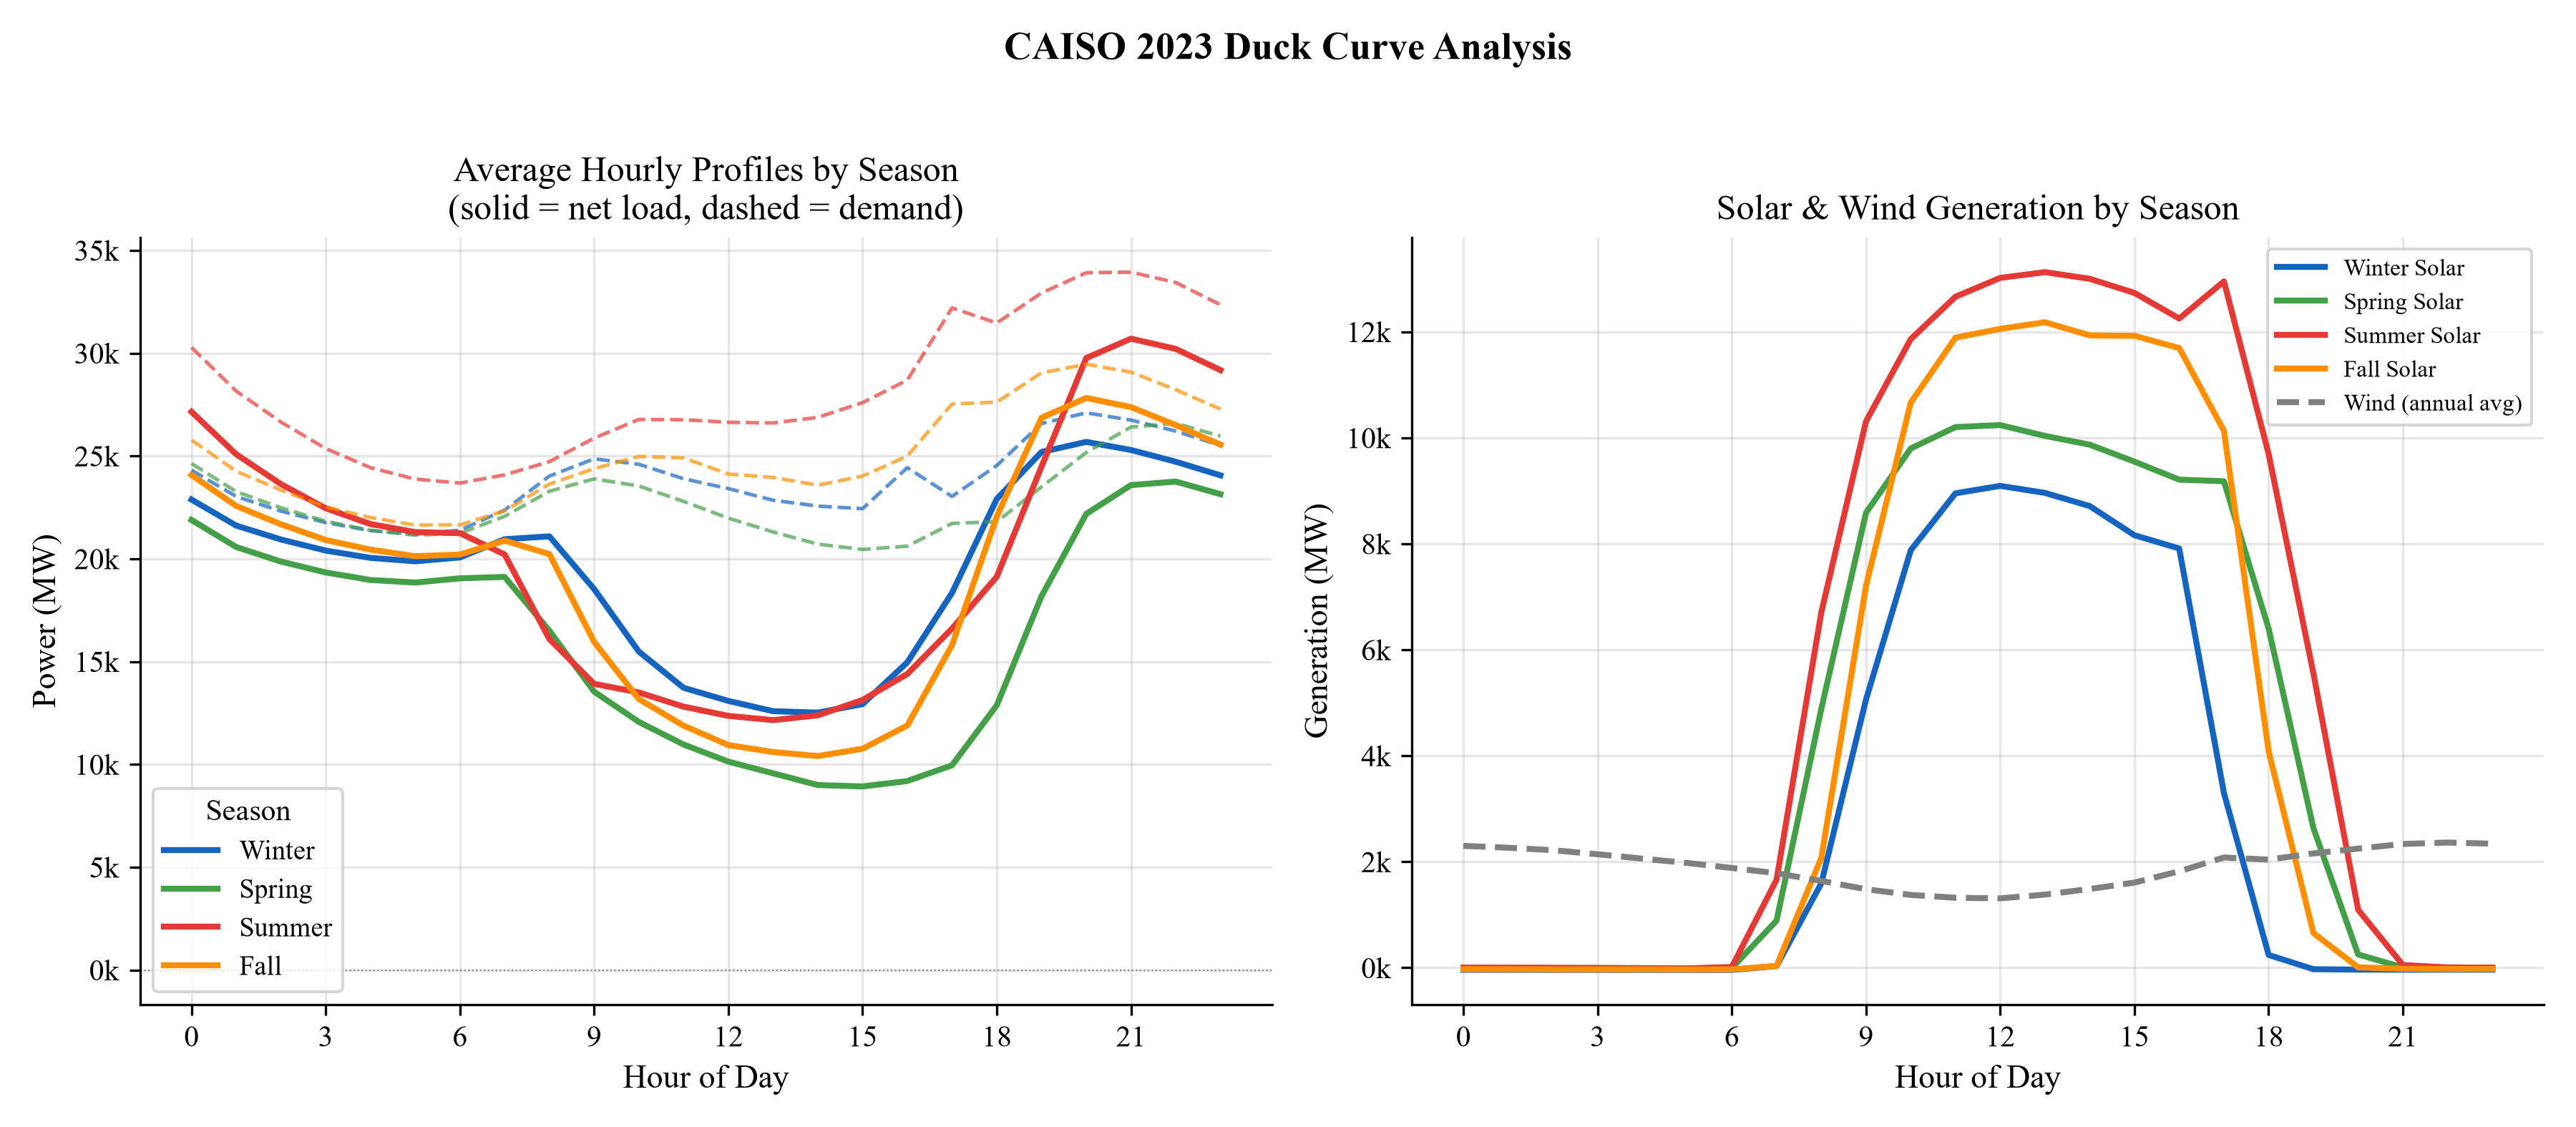
\includegraphics[width=\textwidth]{fig02_duck_curve.png}
\caption{CAISO 2023 duck curve by season (hours in local Pacific time). Left: average hourly net load (solid) vs.\ gross demand (dashed) by season, showing the mid-day belly and evening ramp. Right: average hourly solar generation by season with the annual-average wind profile, the driver of the mid-day net load depression.}
\label{fig:duck}
\end{figure}

Electricity prices are the EIA/ICE SP15 EZ Gen Day-Ahead locational marginal price (LMP) Peak product (234 trading days; range \$9.43--\$348.19/MWh, mean \$63.05, std \$44.65), with non-trading days filled by temporal interpolation. Prices enter the study only as lagged exploratory features and benchmark material (Section~\ref{sec:results_ml}); no daily-to-hourly disaggregation is performed, and the MILP uses fixed technology marginal costs throughout. Temperature data come from the NOAA Integrated Surface Database for three stations (LAX, SFO, Fresno), averaged into a CAISO-wide proxy from which cooling and heating degree hours (CDH/HDH, base 18.3$^\circ$C) are computed.

\subsection{Feature Engineering for Day-Ahead Forecasting}
\label{sec:features}

We adopt a strict day-ahead protocol: at forecast time $T$, only information available before $T$ may be used to predict $P_{\text{net}}(T+24)$. This eliminates all features with lags shorter than 24~hours and rolling statistics computed at the target time. Violations of this constraint, common in the literature, produce artificially inflated metrics ($R^2 > 0.99$) that do not reflect operational performance.

The resulting 35-feature set comprises six categories (Table~\ref{tab:features}): deterministic calendar features with cyclical encodings; the CAISO-published day-ahead gross demand forecast; net load and demand lags at 24/48/72/168~h; solar and wind generation lags (24~h, 168~h); previous-day summary statistics; and trend indicators plus the lagged wholesale price and lagged ISO forecast error. Explicit temperature features (CDH, HDH, and interactions) were evaluated during feature selection but excluded from the final set: lagged demand and net load already embed the demand response to weather, and station temperatures did not improve validation performance. The NOAA data is instead used for error diagnostics (\ref{app:a}), where it shows that the largest errors concentrate on extreme heat days, motivating the weather-ensemble extension discussed in Section~\ref{sec:conclusion}.

\begin{table}[htbp]
\centering
\caption{Feature categories for day-ahead net load forecasting (35 features).}
\label{tab:features}
\small
\resizebox{\textwidth}{!}{%
\begin{tabular}{llp{6.2cm}l}
\toprule
\textbf{Category} & \textbf{Count} & \textbf{Key features} & \textbf{Available at $T$} \\
\midrule
Calendar & 13 & hour, day-of-week, month, day-of-year, weekend flag, week-of-year; sine/cosine encodings & Deterministic \\
ISO forecast & 1 & CAISO day-ahead gross demand forecast & Published before $T$ \\
Load lags & 8 & net load and demand at $t-24/48/72/168$~h & Yes ($\geq 24$~h old) \\
VRE lags & 4 & solar and wind generation at $t-24$, $t-168$~h & Yes \\
Yesterday stats & 6 & demand mean/max/min/std; net load and solar means & Yes \\
Trends and market & 3 & 24-h demand/net load trends; lagged price, lagged ISO forecast error & Yes \\
\bottomrule
\end{tabular}}
\end{table}

Data are split temporally without shuffling: training (January~8 -- August~31, $n = 5{,}664$), validation (September~1 -- October~31, $n = 1{,}464$), and test (November~1 -- December~31, $n = 1{,}345$; 119 hours with missing EIA fuel-type records, 8.1\% of the window, are excluded). The validation set serves two purposes: early stopping during boosting and conformal calibration. The test set is held out entirely from model selection and tuning.

\subsection{Machine Learning Models and Benchmarking}
\label{sec:ml}

Five models are trained. \textbf{LightGBM} \citep{ke2017}: histogram-based gradient boosting, 63 leaves, learning rate 0.03, $L_1/L_2$ regularization, feature/bagging fractions 0.7, up to 3{,}000 iterations with early stopping (patience 100). \textbf{XGBoost} \citep{chen2016}: depth-6 trees, same learning rate, subsampling, and early stopping. \textbf{Random Forest} \citep{breiman2001}: 500 trees, maximum depth 15, minimum 20 samples per leaf. \textbf{LSTM}: best of a manual search over hidden units \{32, 64, 128\}, lookback \{24, 48, 72\}~h, dropout \{0.1, 0.2, 0.3\}, and learning rates \{$10^{-3}$, $3\times10^{-4}$, $10^{-4}$\}; the selected configuration is a 2-layer, 64-unit network with 24-h lookback and cosine-annealed Adam. \textbf{MLP}: three layers (128--64--32, ReLU, Adam).

All models are benchmarked against \textbf{persistence}, $\hat{y}(t) = y(t-24)$, the standard operational baseline \citep{hong2016}. Pairwise comparisons use the Diebold--Mariano test \citep{diebold1995} with Newey--West HAC variance (24 lags). Stability is assessed by five-fold expanding-window cross-validation \citep{bergmeir2012} with fixed 1{,}016-hour test blocks. To contextualize performance, we compute the error of the CAISO-published day-ahead \emph{gross demand} forecast on the same test period: MAE = 1{,}330~MW (MAPE 5.65\% on mean gross demand of 23{,}712~MW), versus our XGBoost net load MAE of 1{,}429~MW, a normalized MAE of 7.4\% on the mean test net load of 19{,}299~MW. (We report normalized MAE rather than MAPE for net load, which is ill-defined when the target crosses zero.) The modest gap reflects the compounded solar and wind uncertainty embedded in the net load target. Temporal generalization is verified by applying the 2023-trained model to all of 2022 ($n = 8{,}593$).

\subsection{Conformalized Quantile Regression}
\label{sec:cqr}

We construct prediction intervals with CQR \citep{romano2019} in three stages. \emph{Stage 1}: five LightGBM quantile models are trained at $\tau \in \{0.10, 0.25, 0.50, 0.75, 0.90\}$ with the pinball loss \citep{gneiting2007}, matching the point-model hyperparameters. LightGBM is used for the quantile stage because it supports the quantile objective natively; its point accuracy is statistically close to XGBoost's ($R^2$ 0.843 vs.\ 0.854), and the conformal step is agnostic to the base learner. \emph{Stage 2}: on the validation set, conformity scores
\begin{equation}
E_i = \max\!\big(\hat{q}_{0.10}(X_i) - Y_i,\; Y_i - \hat{q}_{0.90}(X_i)\big), \qquad i \in \mathcal{D}_{\text{val}},
\end{equation}
measure how far each observation falls outside the uncalibrated interval, and the conformal correction is
\begin{equation}
\hat{Q} = \mathrm{Quantile}\!\left(E_1, \ldots, E_n;\; \tfrac{\lceil(n+1)(1-\alpha)\rceil}{n}\right), \qquad \alpha = 0.10 .
\end{equation}
\emph{Stage 3}: the calibrated 90\% interval for a test point $X$ is
\begin{equation}
\mathcal{C}(X) = \big[\hat{q}_{0.10}(X) - \hat{Q},\; \hat{q}_{0.90}(X) + \hat{Q}\big],
\end{equation}
inheriting both the adaptiveness of quantile regression and the marginal coverage guarantee of conformal prediction. Note that the base pair $(\hat{q}_{0.10}, \hat{q}_{0.90})$ is nominally an 80\% interval; the conformal step recalibrates it to the 90\% target, which is valid because the coverage guarantee derives solely from the conformity-score quantile, not from the nominal levels of the base quantiles \citep{romano2019}. For our application $\hat{Q} = 1{,}044$~MW.

\subsection{MILP Dispatch Formulation}
\label{sec:milp}

We formulate a 168-hour (one-week) economic dispatch as a MILP. The weekly horizon captures the full weekday/weekend periodicity of CAISO net load and BESS cycling: a 24-h horizon undervalues inter-day arbitrage, while annual models sacrifice hourly duck curve dynamics. The formulation is single-bus (copper plate), standard for system-level weekly dispatch studies \citep{jenkins2018,denholm2022b}; this assumption is empirically validated by a two-zone extension below. The model is solved with the open-source HiGHS solver \citep{huangfu2018} via Pyomo \citep{hart2017}.

\textbf{Two-tier gas fleet with unit commitment (UC).} The combined-cycle gas turbine (CCGT) fleet (10{,}000~MW) is represented as two aggregate 5{,}000~MW units with explicit commitment binaries $u^{\text{ccgt}}_{t,k}$ and startup indicators $y^{\text{ccgt}}_{t,k}$: variable cost \$40/MWh, startup cost \$25{,}000/event (${\approx}\$5$/MW warm start; \citealp{nrelatb2023}), minimum load 1{,}500~MW when committed, minimum up/down times of 4~h/2~h, and ramp $\pm 800$~MW/h per unit. Simple-cycle peakers (10{,}000~MW aggregate) are continuous with cost \$65/MWh and ramp $\pm 5{,}000$~MW/h. This two-tier structure exposes the flexibility premium that single-tier gas formulations conceal.

\textbf{Decision variables.} At each hour $t \in \{1,\ldots,168\}$: nuclear output $P_{\text{nuc}}$, CCGT outputs $x^{\text{ccgt}}_{t,k}$, peaker output $P_{\text{peak}}$, BESS charge/discharge $P_{\text{ch}}, P_{\text{dis}}$ and state of charge $\mathrm{SoC}$, imports $P_{\text{imp}}$, exports $P_{\text{exp}}$, load shedding $P_{\text{shed}}$, curtailment $P_{\text{curt}}$, and the binary BESS mode $u_t$.

\textbf{Objective.} Minimize total system cost:
\begin{multline}
\label{eq:obj}
\min \sum_{t=1}^{T} \Big[ c_{\text{nuc}} P_{\text{nuc}}(t) + c_{\text{ccgt}} \!\sum_k x^{\text{ccgt}}_{t,k} + c^{\text{su}} \!\sum_k y^{\text{ccgt}}_{t,k} + c_{\text{peak}} P_{\text{peak}}(t) \\
+\ c_{\text{bess}}\big(P_{\text{ch}} + P_{\text{dis}}\big) + c_{\text{imp}} P_{\text{imp}} - r_{\text{exp}} P_{\text{exp}} + V P_{\text{shed}} + c_{\text{curt}} P_{\text{curt}} \Big]
\end{multline}
with $c_{\text{nuc}} = 12$, $c_{\text{ccgt}} = 40$, $c_{\text{peak}} = 65$, $c_{\text{bess}} = 5$, $c_{\text{imp}} = 55$, $r_{\text{exp}} = 20$, $c_{\text{curt}} = 10$~\$/MWh, $c^{\text{su}} = \$25{,}000$/start, and value of lost load $V = 10{,}000$~\$/MWh; variable-cost levels follow standard technology assumptions \citep{nrelatb2023}, with the import price and gas price varied parametrically in Section~\ref{sec:sensitivity}.

\textbf{Constraints.}
(C1)~Power balance: $P_{\text{nuc}} + \sum_k x^{\text{ccgt}}_{t,k} + P_{\text{peak}} + P_{\text{dis}} + P_{\text{imp}} + P_{\text{shed}} = P_{\text{net}}(t) + P_{\text{ch}} + P_{\text{exp}} + P_{\text{curt}}$.
(C2)~BESS dynamics: $\mathrm{SoC}(t) = \mathrm{SoC}(t{-}1) + \sqrt{\eta}\,P_{\text{ch}}(t) - P_{\text{dis}}(t)/\sqrt{\eta}$ with round-trip $\eta = 0.90$ and $\mathrm{SoC}(0) = 0.5\,\bar{E}$, where $\bar{E}$ denotes the BESS energy capacity (20~GWh baseline).
(C3)~End-of-horizon SoC floor $\mathrm{SoC}(T) \geq 0.35\,\bar{E}$, preventing the optimizer from gaming the finite horizon by draining the battery in the final hours \citep{sioshansi2009}.
(C4)~BESS mutual exclusion via big-M with binary $u_t$.
(C5)~Nuclear ramp $\pm 100$~MW/h, the load-following limit of pressurized water reactors (${\sim}4.4\%$/h of rated capacity; \citealp{nea2011}).
(C6)~CCGT unit commitment: $1{,}500\,u^{\text{ccgt}}_{t,k} \leq x^{\text{ccgt}}_{t,k} \leq 5{,}000\,u^{\text{ccgt}}_{t,k}$; startup logic $y^{\text{ccgt}}_{t,k} \geq u^{\text{ccgt}}_{t,k} - u^{\text{ccgt}}_{t-1,k}$; minimum up/down times; ramp $\pm 800$~MW/h with startup exemption.
(C7)~Peaker ramp $\pm 5{,}000$~MW/h.
(C8)~SoC bounds $0.10\,\bar{E} \leq \mathrm{SoC}(t) \leq 0.90\,\bar{E}$.
(C9)~Capacity bounds: nuclear 1{,}800--2{,}256~MW (Diablo Canyon), imports $\leq 10{,}000$~MW, exports $\leq 6{,}000$~MW.
Explicit spinning-reserve constraints are omitted: at the peak of the representative summer week (Aug~7--13; Section~\ref{sec:results_seasonal}), committed capacity (37{,}256~MW) barely exceeds net load (36{,}999~MW), so a percentage reserve requirement would force artificial shedding. More starkly, at the true annual net load peak (44{,}900~MW, mid-July; Section~\ref{sec:fullyear}), the stylized fleet's aggregate capacity is a \emph{shortfall}, not a margin, reinforcing rather than undermining this modeling choice, since a formal reserve requirement would only worsen an already capacity-constrained extreme week. In practice CAISO procures reserves and manages such extremes through mechanisms outside this weekly aggregate model (demand response, emergency imports, hydro dispatch; \citealp{caiso2023}), as discussed in Section~\ref{sec:fullyear}.

The model contains ${\sim}2{,}700$ variables (840 binary: 168 BESS mode, $2\times168$ CCGT commitment, $2\times168$ CCGT startup) and ${\sim}3{,}700$ constraints; all instances solve to global optimality (gap $< 0.01\%$) in well under 1~s (0.4--0.5~s typical).

\textbf{CQR-driven robust scenarios.} The CQR interval defines a data-driven box uncertainty set: $P_{\text{net}}(t,\gamma) = \hat{P}(t) + \gamma\,[\hat{q}_{0.90}(t) - \hat{P}(t)]$, implementing the budget-of-uncertainty framework of \citet{bertsimas2004}. Because all dispatch decisions are here-and-now (no recourse) and both cost and the binding power-balance constraint are monotone in net load, the worst case over the box $[\hat{q}_{0.10}, \hat{q}_{0.90}]$ is attained at the upper bound; solving the deterministic MILP at the $\gamma$-scaled upper profile is therefore the \emph{exact} static robust counterpart, not a heuristic approximation. Although the point forecast (XGBoost) and the conformalized quantiles (LightGBM) come from different learners, the set is well defined in practice: $\hat{q}_{0.10}(t) \leq \hat{P}(t) \leq \hat{q}_{0.90}(t)$ holds in all 1{,}345 test hours, so the $\gamma$-scaled band never inverts. Six scenarios are evaluated: S1 ($\gamma{=}0$, deterministic point forecast), S2 ($\gamma{=}1$, worst-case Q90), S3 (best-case Q10), S4 (no nuclear), S5 (small BESS, 1~GW/4~GWh), and S6 ($\gamma{=}0.5$, robust blend). A systematic sweep $\gamma \in \{0, 0.25, 0.5, 0.75, 1\}$ (Section~\ref{sec:gamma}) cross-validates S1, S6, and S2.

\textbf{Emissions accounting.} CO$_2$ is computed ex post from the optimal dispatch using technology-specific factors: 0.37~t/MWh for CCGTs (heat rate ${\sim}7.0$~MMBtu/MWh at 53.07~kg/MMBtu; \citealp{epa2023}), 0.55~t/MWh for peakers (${\sim}10.5$~MMBtu/MWh), and 0.428~t/MWh for imports (the California Air Resources Board default emission factor for unspecified imported electricity \citep{carb2023}, a deliberately conservative regulatory convention). Nuclear, BESS throughput, and renewables are assigned zero operational emissions.

\textbf{Stochastic programming baseline.} To benchmark the CQR-robust approach against the classical alternative, we formulate a two-stage stochastic program on the \emph{same information set}. The scenario set is the CQR triplet $\{\hat{q}_{0.10}, \hat{P}, \hat{q}_{0.90}\}$ with Swanson--Megill probabilities $\{0.30, 0.40, 0.30\}$, the standard three-point approximation for P10/P50/P90 fractiles \citep{keefer1983}. First-stage (here-and-now) decisions are the inflexible ones: CCGT commitment and startup binaries and the nuclear trajectory; all continuous dispatch (CCGT output levels, peakers, BESS, imports/exports, shedding, curtailment) is second-stage recourse per scenario. All plans (deterministic, robust ($\gamma = 0.5, 1$), and SP) are then evaluated \emph{out of sample} under an identical protocol: their first-stage decisions are frozen and the recourse problem is re-solved against the realized net load, yielding realized costs that are directly comparable across planning paradigms.

\textbf{Two-zone validation.} To validate the copper-plate assumption, a two-zone (NP15/SP15) extension adds the Path~15 interface constraint (4{,}500~MW forward / 3{,}500~MW reverse; \citealp{caiso2023}) with proportionally allocated capacities. The two-zone dispatch costs \$43.73/MWh versus \$42.15/MWh for the copper plate ($+3.7\%$; both computed on the realized November-week net load, hence the \$42.15 basis rather than S1's \$41.84 planning cost); Path~15 flows average 24.3\% of rating and bind in 0 of 168 hours. Because the scenario \emph{comparisons} central to this study (e.g., S4$-$S1) difference out any residual inter-zonal effects, the single-bus formulation is adequate for our purposes.


%% ====================================================================
\section{Results}
\label{sec:results}
%% ====================================================================

\subsection{Generation Mix and Duck Curve Formation}
\label{sec:results_data}

Fig.~\ref{fig:genmix} shows the hourly generation mix during a representative spring week (April 10--16, 2023). Solar (up to 16{,}000~MW) dominates mid-day production; nuclear holds constant at 2{,}256~MW; and as solar declines in late afternoon, gas ramps from ${\sim}2{,}000$~MW to over 15{,}000~MW within 4--5 hours, the duck curve's ``neck.'' During this week the realized net load reaches $-2{,}852$~MW.

\begin{figure}[htbp]
\centering
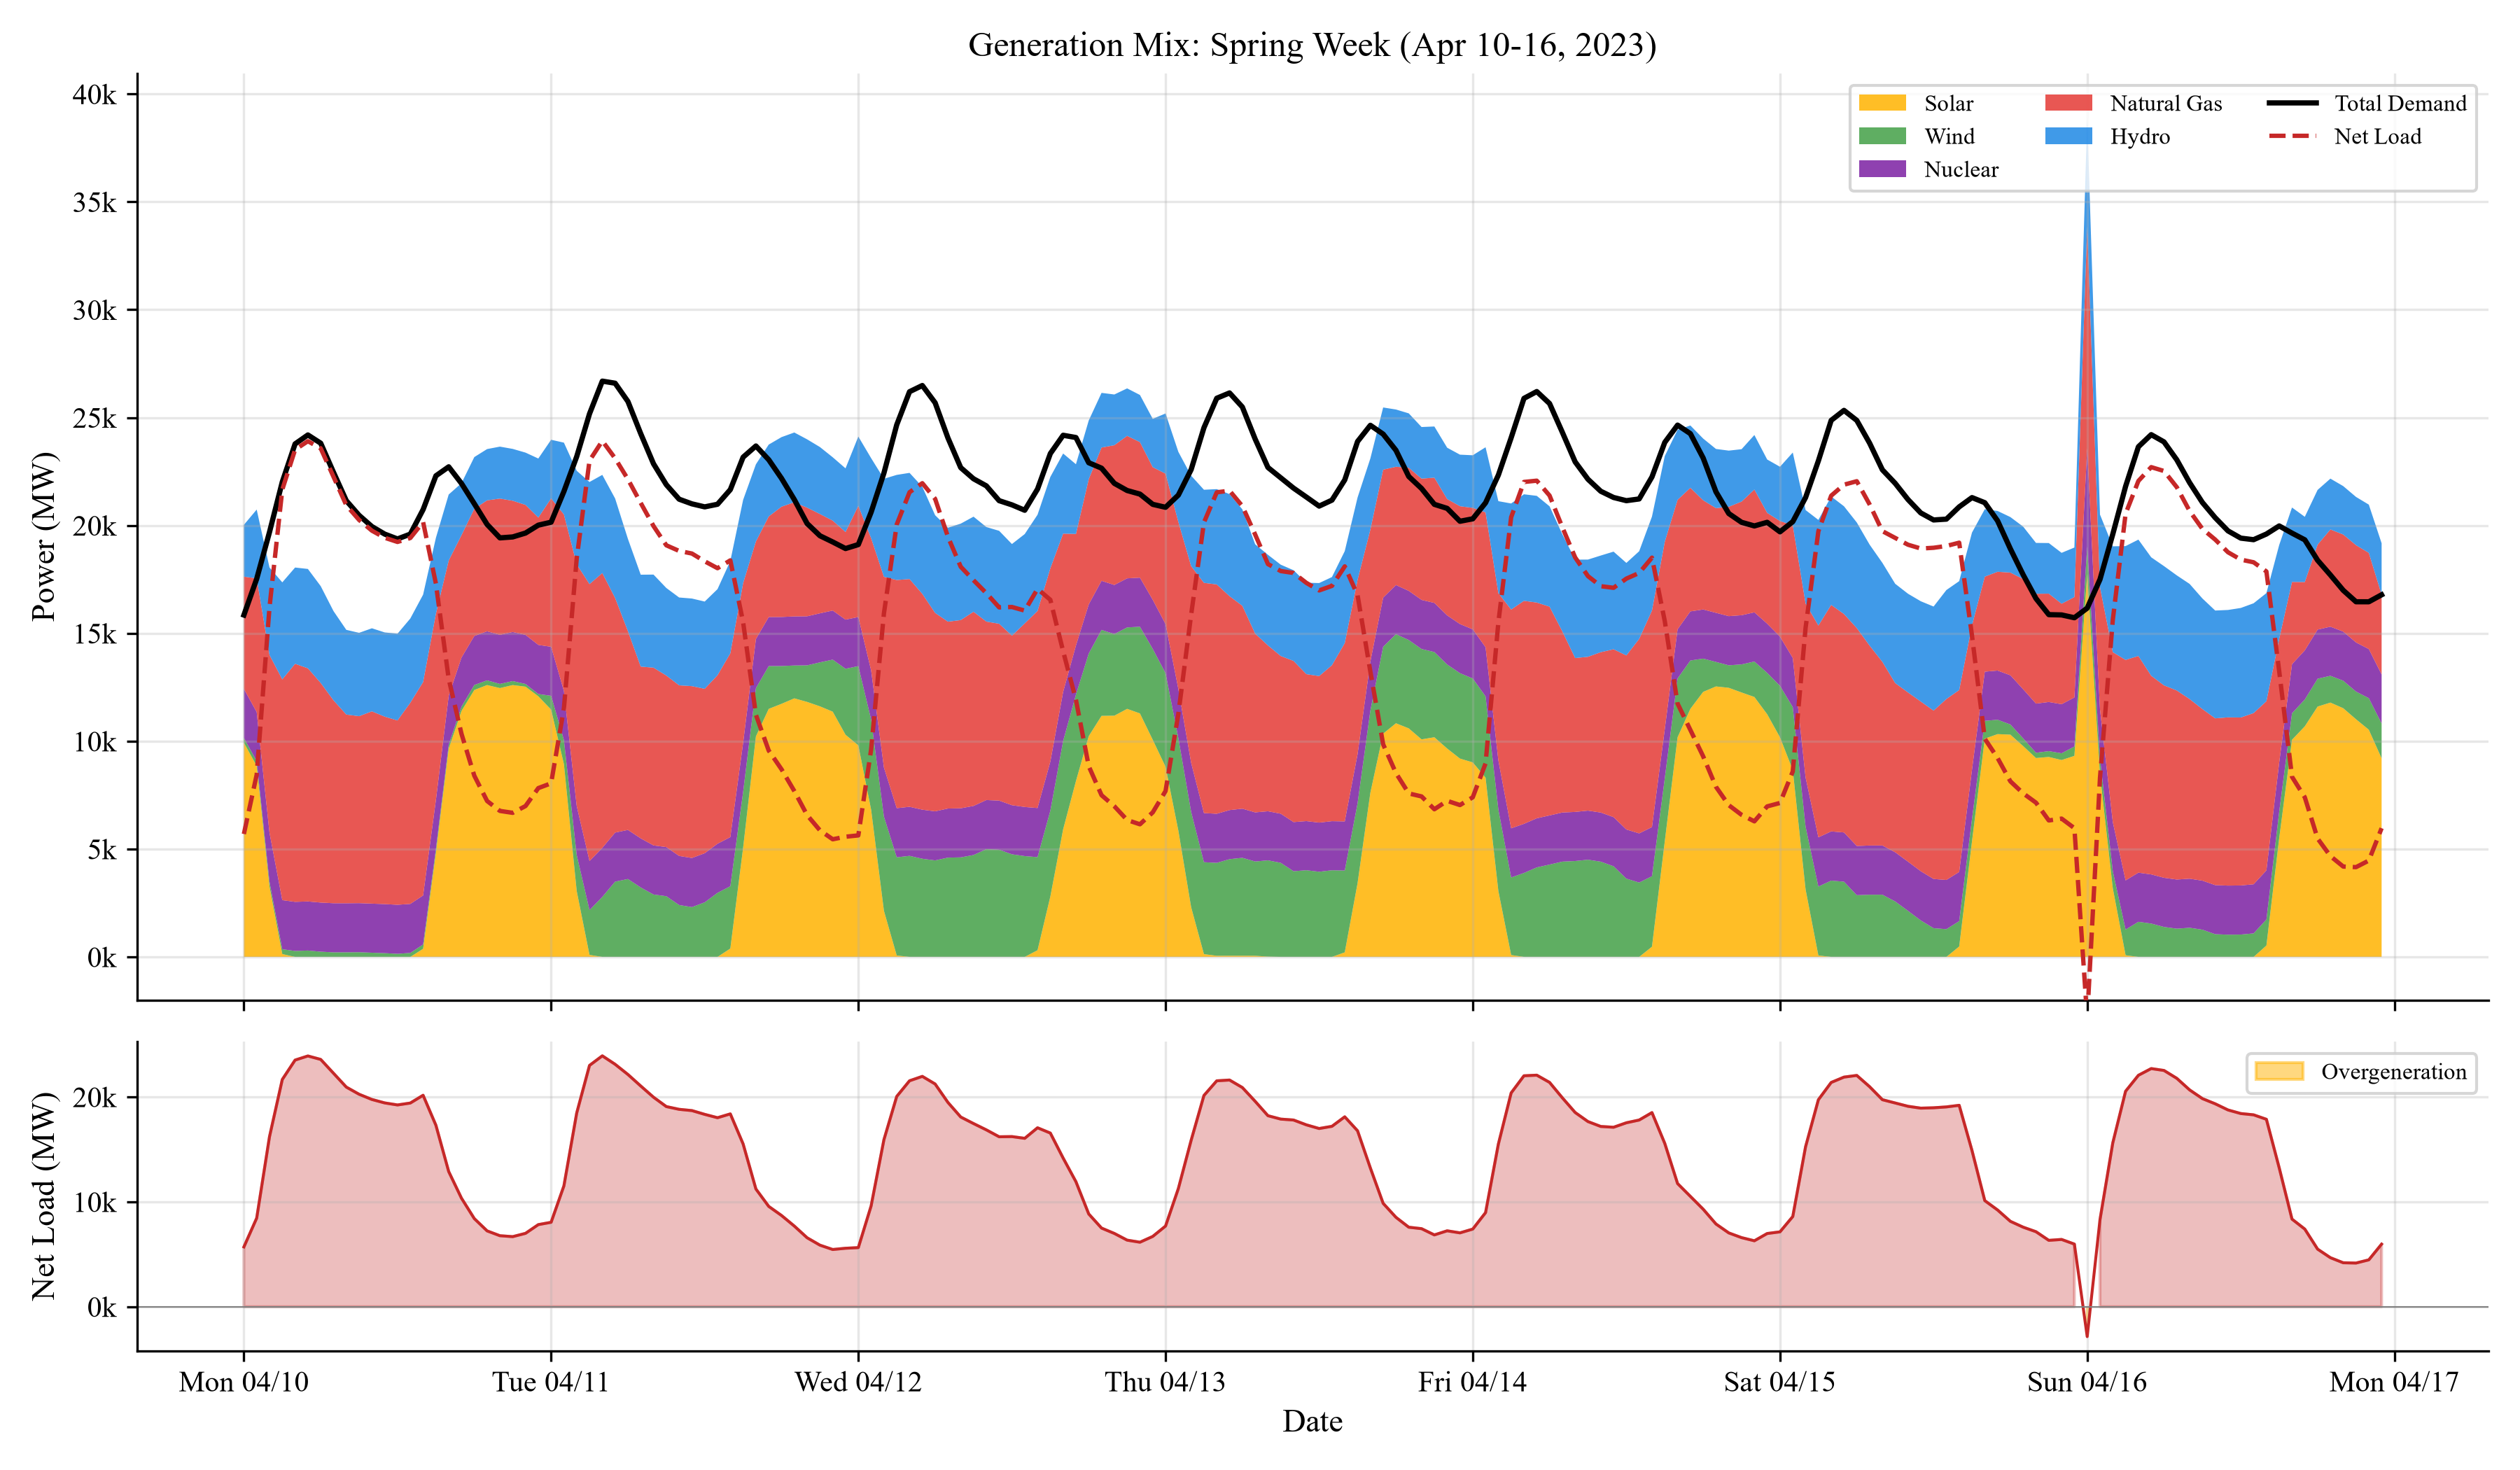
\includegraphics[width=\textwidth]{fig03_generation_mix_spring_week.png}
\caption{CAISO generation mix during a spring week (April 10--16, 2023), showing duck curve formation: solar dominates mid-day, nuclear provides constant baseload, gas handles the evening ramp.}
\label{fig:genmix}
\end{figure}

\subsection{Net Load Forecasting Performance}
\label{sec:results_ml}

Table~\ref{tab:benchmark} summarizes day-ahead performance on the held-out test set. XGBoost achieves the best results ($R^2 = 0.854$, MAE = 1{,}429~MW, RMSE = 2{,}071~MW), a forecast skill of $+18.5\%$ over persistence. All three ensemble models beat persistence at the 0.1\% level; XGBoost is statistically superior to both Random Forest (DM $p = 0.026$) and LightGBM (DM $p < 0.001$).

\begin{table}[htbp]
\centering
\caption{Day-ahead net load forecasting benchmark (test set: November--December 2023). DM test against persistence.}
\label{tab:benchmark}
\small
\resizebox{\textwidth}{!}{%
\begin{tabular}{lrrrrrl}
\toprule
\textbf{Model} & \textbf{MAE (MW)} & \textbf{RMSE (MW)} & \textbf{$R^2$} & \textbf{Train $R^2$} & \textbf{Gap} & \textbf{DM $p$} \\
\midrule
LightGBM        & 1{,}565 & 2{,}146 & 0.843 & 0.997 & 0.154 & $< 0.001$ \\
\textbf{XGBoost} & \textbf{1{,}429} & \textbf{2{,}071} & \textbf{0.854} & 0.972 & 0.118 & $< 0.001$ \\
Random Forest   & 1{,}533 & 2{,}211 & 0.834 & 0.947 & 0.113 & $< 0.001$ \\
LSTM (2-layer)  & 2{,}278 & 3{,}085 & 0.676 & 0.924 & 0.248 & $< 0.001$ \\
MLP (3-layer)   & 3{,}220 & 3{,}904 & 0.481 & 0.996 & 0.514 & $< 0.001$ \\
Persistence     & 1{,}753 & 2{,}783 & 0.736 & ---   & ---   & baseline \\
\bottomrule
\end{tabular}}
\end{table}

The deep learning baselines underperform even persistence: the LSTM's overfit gap (train $R^2 = 0.924$ vs.\ test 0.676) indicates that ${\sim}5{,}700$ training samples are insufficient for a recurrent architecture to learn generalizable temporal dependencies, while the MLP overfits severely (gap 0.514). This confirms, for the tested recurrent and feedforward architectures, the documented advantage of GBM on moderate-scale tabular energy data \citep{hertel2022,grinsztajn2022}; we do not exclude that attention-based architectures with larger training corpora could close the gap.

Out-of-sample temporal generalization is confirmed by applying the 2023-trained LightGBM to calendar year 2022: $R^2 = 0.908$, MAE = 1{,}514~MW over 8{,}593 hours. Because 2022 wholesale price data were not available at the time of this validation, the single lagged-price feature (\texttt{price\_lag24h}) is set to zero for the 2022 run; given its minor contribution to the trained model (1.1\% of total feature-importance gain, Appendix Fig.~\ref{fig:featimp}), this substitution is expected to have negligible impact on the reported 2022 metrics. Part of the higher 2022 $R^2$ reflects an intrinsically more predictable year (persistence itself improves from 0.736 to 0.822); the relevant evidence is that the model's \emph{skill over persistence} is preserved out of year (MAE gain of the same LightGBM model: $+21.6\%$ in 2022 vs.\ $+14.1\%$ on the 2023 test set), indicating durable seasonal and diurnal structure rather than year-specific artifacts.

\emph{Note on price forecasting.} Preliminary experiments applying the same framework to daily SP15 prices showed no ML model outperforming persistence (best ML MAE \$6.5 vs.\ persistence \$4.5/MWh), consistent with the electricity price forecasting literature \citep{weron2014,lago2021}. Since the MILP uses fixed marginal costs, standard in dispatch optimization, price forecasting is excluded from the pipeline.

\subsection{Cross-Validation and Model Stability}
\label{sec:results_cv}

Five-fold expanding-window cross-validation confirms framework stability across seasonal regimes (mean $R^2 = 0.869 \pm 0.089$). The single exception, Fold~2, coincides with the 2023 California heat events; the full fold-by-fold breakdown and the associated temperature-error analysis are reported in \ref{app:a} (Table~\ref{tab:cv}, Fig.~\ref{fig:errtemp}) to keep the main results focused on headline findings.

\subsection{Prediction Intervals and Conformal Calibration}
\label{sec:results_pi}

CQR produces well-calibrated intervals: the 90\% PI achieves 88.8\% empirical coverage (within finite-sample variation for $n = 1{,}345$) with mean width 5{,}182~MW, conformal correction $\hat{Q} = 1{,}044$~MW, and a mean interval (Winkler) score \citep{gneiting2007} of 8{,}346~MW at $\alpha = 0.10$. The conformal step is not cosmetic: the uncalibrated quantile-regression interval achieves only 61.1\% empirical coverage (width 3{,}094~MW) with a \emph{worse} Winkler score of 10{,}874~MW: conformalization therefore improves the interval under a proper scoring rule while restoring near-nominal coverage, rather than merely trading width for coverage (Table~\ref{tab:qrcqr}). Fig.~\ref{fig:pred} shows that the intervals are adaptive, widening during rapid ramps and narrowing during stable hours.

Marginal coverage, however, does not imply conditional coverage, and we report the gap honestly. Fig.~\ref{fig:confdiag} disaggregates coverage by hour of day: mid-day hours are over-covered (up to 100\%) while evening-ramp hours (16:00--22:00) fall to 78.6--84\%, precisely when net load uncertainty matters most for dispatch. This heterogeneity is expected (split-conformal methods guarantee only marginal coverage \citep{romano2019}), and it does not undermine the robust MILP, whose $\gamma$-parameterization hedges against the upper bound irrespective of when misses occur. It does, however, sharpen the case for the adaptive and time-conditional conformal extensions \citep{gibbs2021,zaffran2022} identified in Section~\ref{sec:conclusion}.

\begin{figure}[htbp]
\centering
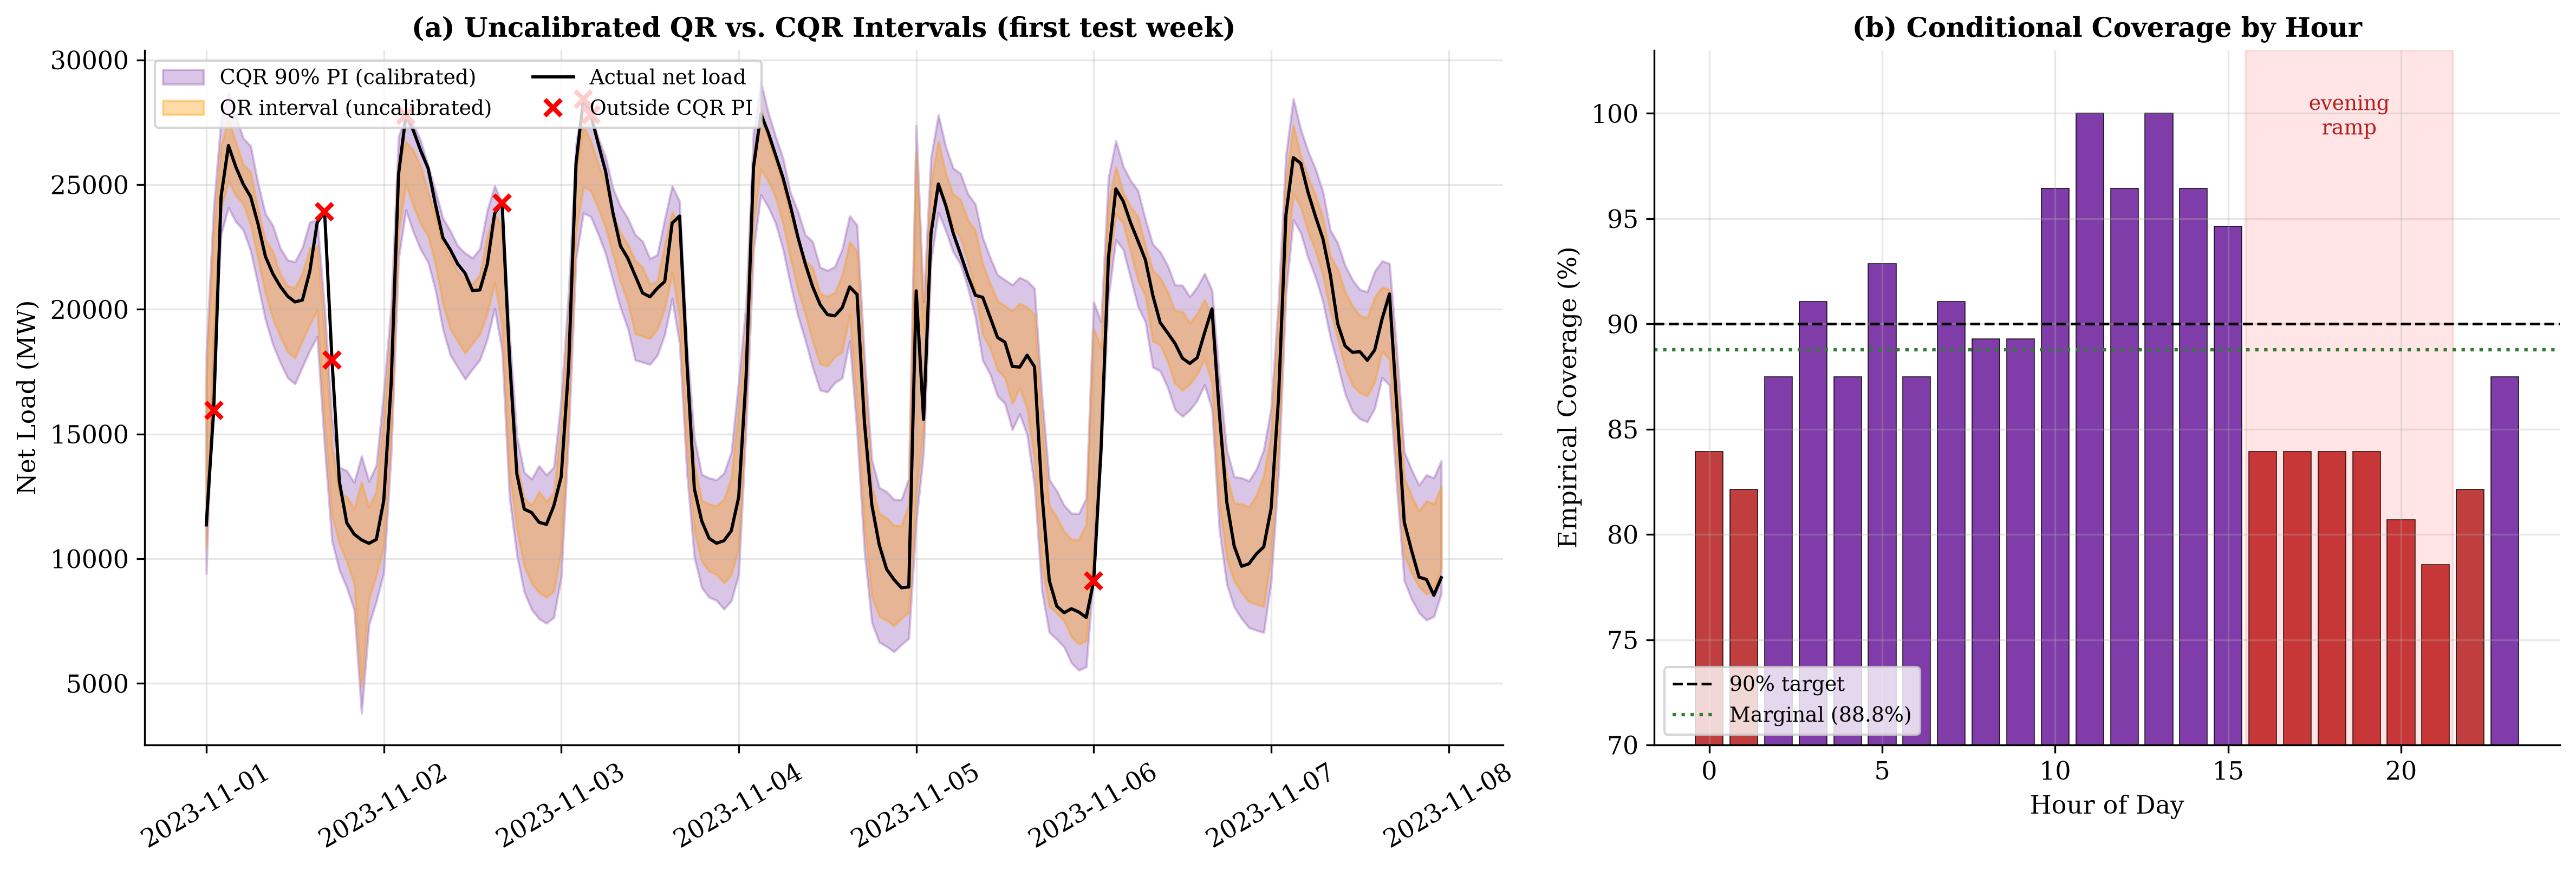
\includegraphics[width=\textwidth]{fig_conformal_diagnostics.png}
\caption{Conformal calibration diagnostics. (a) Uncalibrated QR vs.\ calibrated CQR intervals over the first test week; red crosses mark observations outside the CQR interval. (b) Conditional coverage by hour of day: evening-ramp hours (shaded) are under-covered relative to the 90\% target, while mid-day hours are over-covered.}
\label{fig:confdiag}
\end{figure}

\begin{table}[htbp]
\centering
\caption{Value of conformalization: uncalibrated quantile regression vs.\ CQR (net load, test set, 90\% target).}
\label{tab:qrcqr}
\small
\resizebox{\textwidth}{!}{%
\begin{tabular}{lrrr}
\toprule
\textbf{Interval} & \textbf{Coverage (\%)} & \textbf{Mean width (MW)} & \textbf{Winkler score (MW)} \\
\midrule
QR (uncalibrated, $\hat{q}_{0.10}$--$\hat{q}_{0.90}$) & 61.1 & 3{,}094 & 10{,}874 \\
CQR (conformalized) & 88.8 & 5{,}182 & 8{,}346 \\
\bottomrule
\end{tabular}}
\end{table}

\begin{figure}[htbp]
\centering
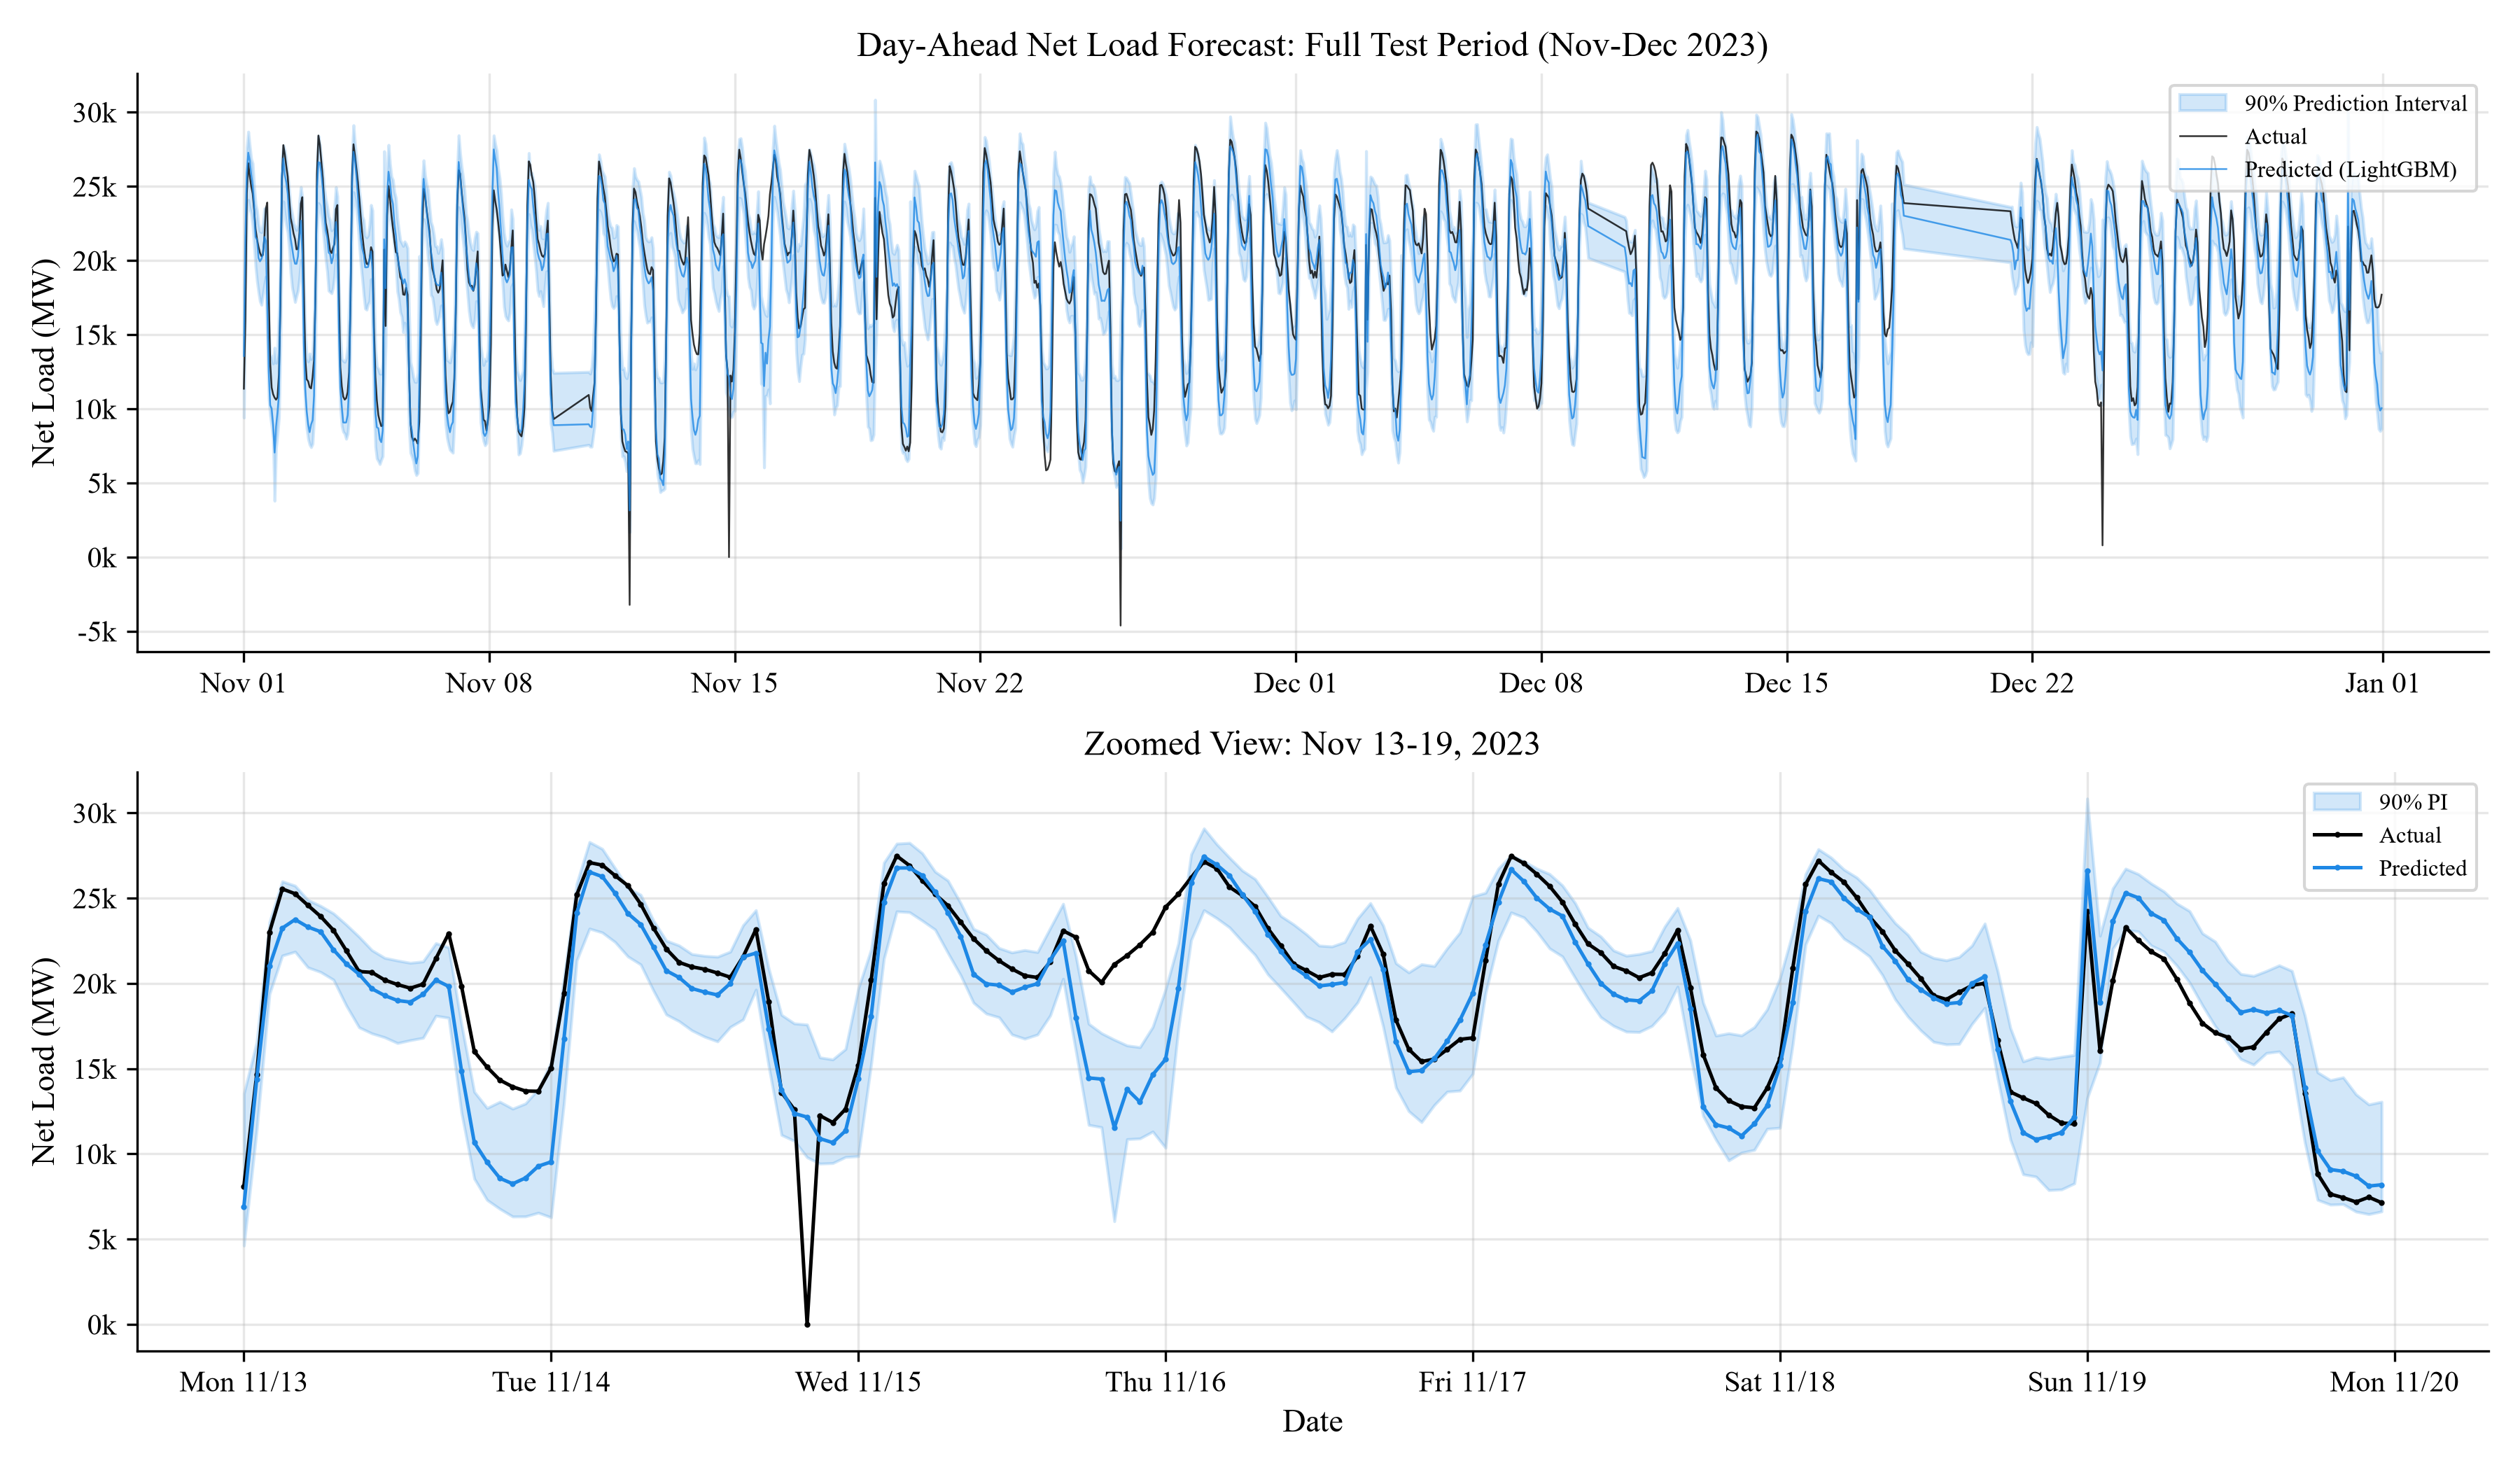
\includegraphics[width=\textwidth]{fig07_netload_prediction_PI.png}
\caption{Day-ahead net load forecast with 90\% CQR prediction intervals. Top: full test period. Bottom: a representative test week (November 13--19) showing interval adaptiveness.}
\label{fig:pred}
\end{figure}

Formal residual diagnostics (skewness, kurtosis, normality, and autocorrelation tests) and a hyperparameter sensitivity analysis are reported in \ref{app:a} (Tables~\ref{tab:diag}--\ref{tab:hyper}); both confirm well-behaved, distribution-appropriate residuals and a model choice that is not overly sensitive to hyperparameter selection.

\subsection{Dispatch Optimization Results}
\label{sec:results_milp}

Table~\ref{tab:scenarios} presents the six core scenarios on the November test week; all solve to global optimality in well under 1~s (0.4--0.5~s typical). Key findings: (i)~removing nuclear (S4 vs.\ S1) raises unit cost by \$5.51/MWh ($+13.2\%$), compensated by near-maximal CCGT output (9{,}987~MW), an eightfold increase in expensive peaker dispatch (144 $\to$ 1{,}153~MW average), and higher imports; (ii)~the robust dispatch (S6) costs $+1.9\%$ over deterministic, with the two-tier model revealing the true flexibility premium of pre-scheduled peakers; (iii)~shrinking BESS to 1~GW (S5) adds only $0.8\%$ to cost (\$41.84 $\to$ \$42.16/MWh) but leaves the battery near depletion (end SoC 7\% of the 20~GWh reference); (iv)~zero shedding and curtailment across all scenarios confirm the November week lies within the operational envelope. The sharp drop in BESS cycling under the pessimistic profiles (S2: 0.44 cycles/week vs.\ S1: 4.94) has a simple mechanism: hedging pre-schedules additional CCGT and peaker output across all hours, which flattens the residual intra-day price differential that arbitrage exploits, so robustness crowds out storage utilization. Fig.~\ref{fig:dispatch} shows the S1 dispatch stack.

\begin{table}[htbp]
\centering
\caption{MILP scenario comparison (168-h dispatch, November 2023). Two-tier gas: CCGT (\$40/MWh, $\pm$800~MW/h, UC) + peakers (\$65/MWh, $\pm$5{,}000~MW/h). End-of-horizon SoC $\geq$ 35\% enforced.}
\label{tab:scenarios}
\small
\resizebox{\textwidth}{!}{%
\begin{tabular}{lrrrrrrr}
\toprule
\textbf{Scenario} & \textbf{\$/MWh} & \textbf{CCGT} & \textbf{Peaker} & \textbf{Import} & \textbf{Shed} & \textbf{Cycles} & \textbf{SoC$_{\text{end}}$} \\
 & & \textbf{(MW)} & \textbf{(MW)} & \textbf{(MW)} & \textbf{(MWh)} & \textbf{(/wk)} & \textbf{(\%)} \\
\midrule
S1 Deterministic ($\gamma{=}0$) & 41.84 & 9{,}734 & 144 & 5{,}716 & 0 & 4.94 & 35 \\
S2 Worst-case ($\gamma{=}1$)    & 43.59 & 10{,}000 & 1{,}275 & 7{,}155 & 0 & 0.44 & 35 \\
S3 Best-case (Q10)              & 40.25 & 9{,}036 & 0 & 4{,}213 & 0 & 3.25 & 35 \\
S4 No Nuclear                   & 47.35 & 9{,}987 & 1{,}153 & 6{,}678 & 0 & 2.51 & 35 \\
S5 Small BESS (1 GW)            & 42.16 & 9{,}274 & 543 & 5{,}769 & 0 & 5.18 & 7 \\
S6 Robust ($\gamma{=}0.5$)      & 42.63 & 9{,}989 & 641 & 6{,}380 & 0 & 2.54 & 35 \\
\bottomrule
\end{tabular}}
\end{table}

\begin{figure}[htbp]
\centering
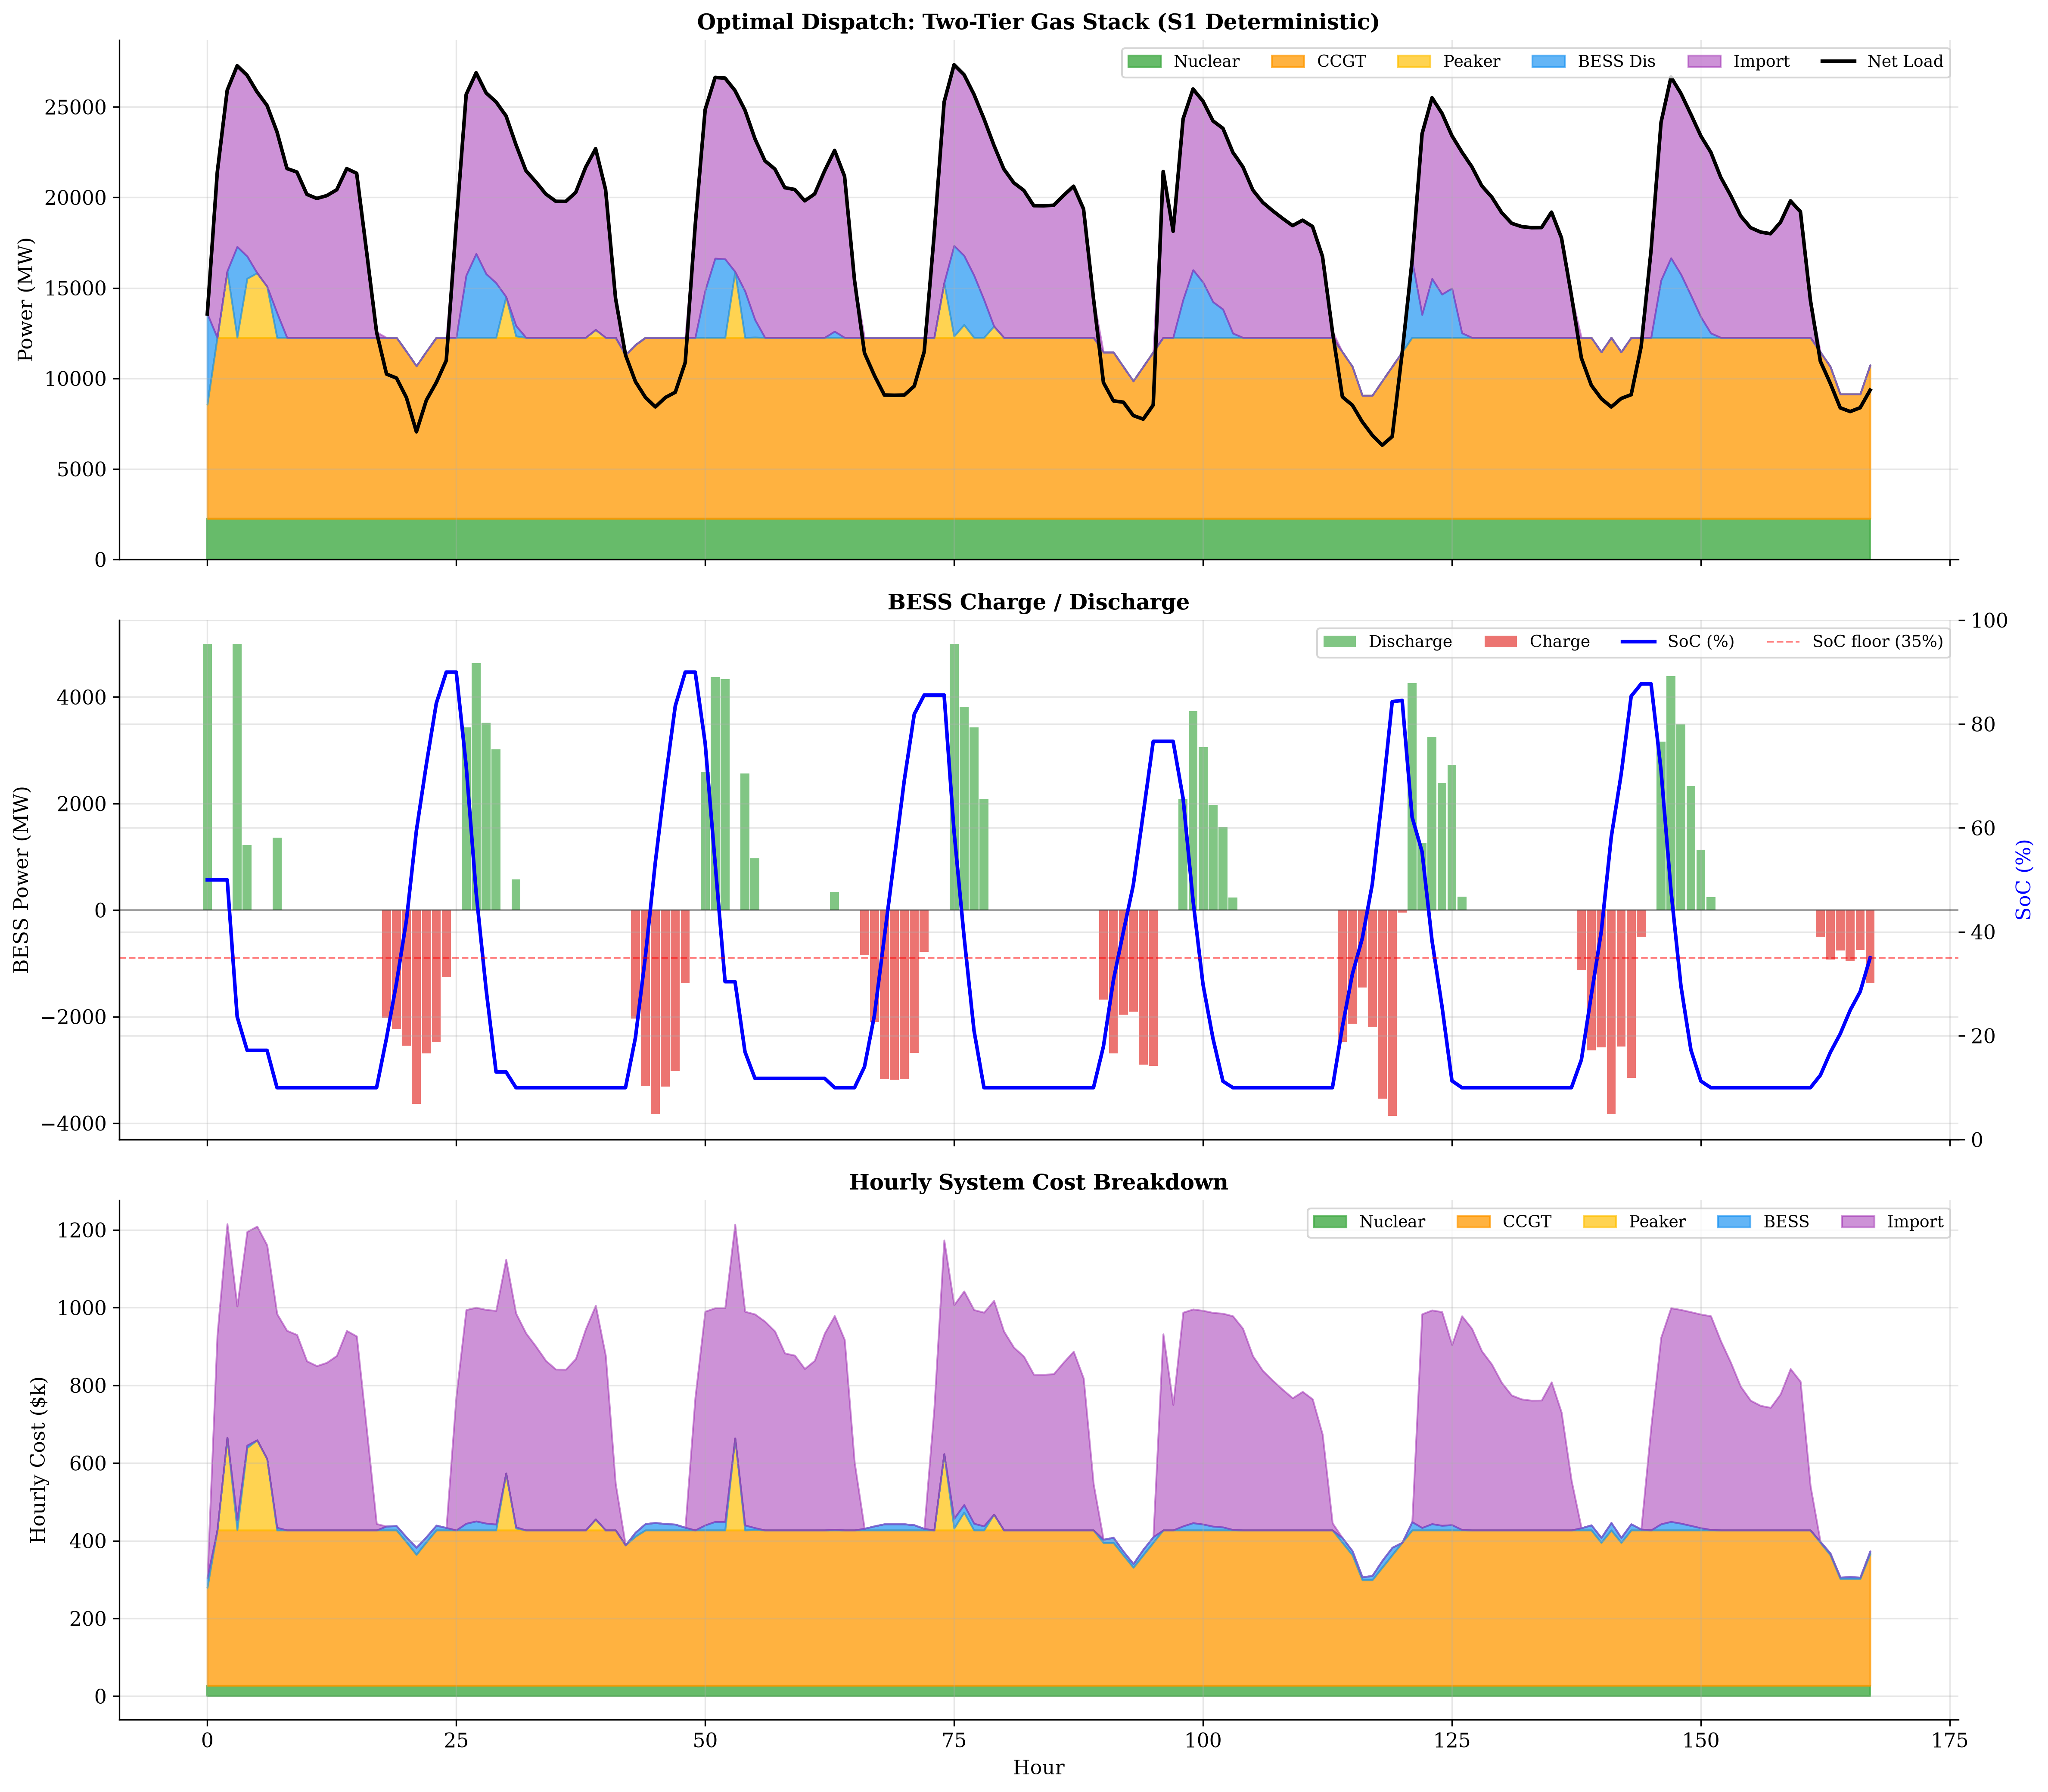
\includegraphics[width=\textwidth]{fig13_dispatch_stack.png}
\caption{Optimal dispatch for S1 (deterministic, two-tier gas). Top: generation stack. Middle: BESS charge/discharge with state of charge and end-of-horizon floor. Bottom: hourly cost breakdown.}
\label{fig:dispatch}
\end{figure}

\subsection{Four-Season Dispatch Analysis}
\label{sec:results_seasonal}

The MILP is run on four representative weeks with realized net load, selected ex ante by transparent criteria: the spring week (April 10--16) exhibits the deepest sustained duck-belly conditions among the four selected weeks (weekly net load minimum $-2{,}852$~MW; the annual minimum of $-10{,}369$~MW occurs in early July and is covered by the annual sweep of Section~\ref{sec:fullyear}), the summer week (August 7--13) is a typical high-demand summer week (peak net load 36{,}999~MW), and the winter and fall weeks are typical mid-season weeks with no holidays. The results (Table~\ref{tab:seasons}, Fig.~\ref{fig:seasons}) yield a consistent cost ordering: summer (\$45.16/MWh, sustained 2{,}604~MW peaker deployment) $>$ winter (\$42.27) $\approx$ fall (\$42.15) $>$ spring (\$39.85, zero peakers; duck-belly hours charge the BESS at low marginal cost). CCGT commitment reflects seasonal shape: summer holds both units online continuously (0 starts) while spring requires 4 start--stop cycles to avoid minimum-load violations during the duck belly. Zero shedding across all four selected seasonal weeks confirms system adequacy with nuclear online under typical conditions; the annual net load maximum (44{,}900~MW, mid-July) falls outside this typical-week sample and is analyzed separately as a capacity-stress event in Section~\ref{sec:fullyear}.

\begin{table}[htbp]
\centering
\caption{Four-season dispatch (realized CAISO net load, with nuclear).}
\label{tab:seasons}
\small
\resizebox{\textwidth}{!}{%
\begin{tabular}{lrrrrrrr}
\toprule
\textbf{Season (week)} & \textbf{NL mean} & \textbf{NL range} & \textbf{\$/MWh} & \textbf{CCGT} & \textbf{Peaker} & \textbf{Starts} & \textbf{Shed} \\
 & \textbf{(MW)} & \textbf{(MW)} & & \textbf{(MW)} & \textbf{(MW)} & & \textbf{(MWh)} \\
\midrule
Winter (Jan 23--29) & 18{,}851 & 9{,}089--27{,}383 & 42.27 & 9{,}939 & 402 & 2 & 0 \\
Spring (Apr 10--16) & 14{,}439 & $-2{,}852$--23{,}919 & 39.85 & 8{,}504 & 0 & 4 & 0 \\
Summer (Aug 7--13)  & 22{,}366 & 11{,}285--36{,}999 & 45.16 & 10{,}000 & 2{,}604 & 0 & 0 \\
Fall (Nov 1--7)     & 18{,}407 & 7{,}648--28{,}430 & 42.15 & 9{,}793 & 450 & 2 & 0 \\
\bottomrule
\end{tabular}}
\end{table}

\begin{figure}[htbp]
\centering
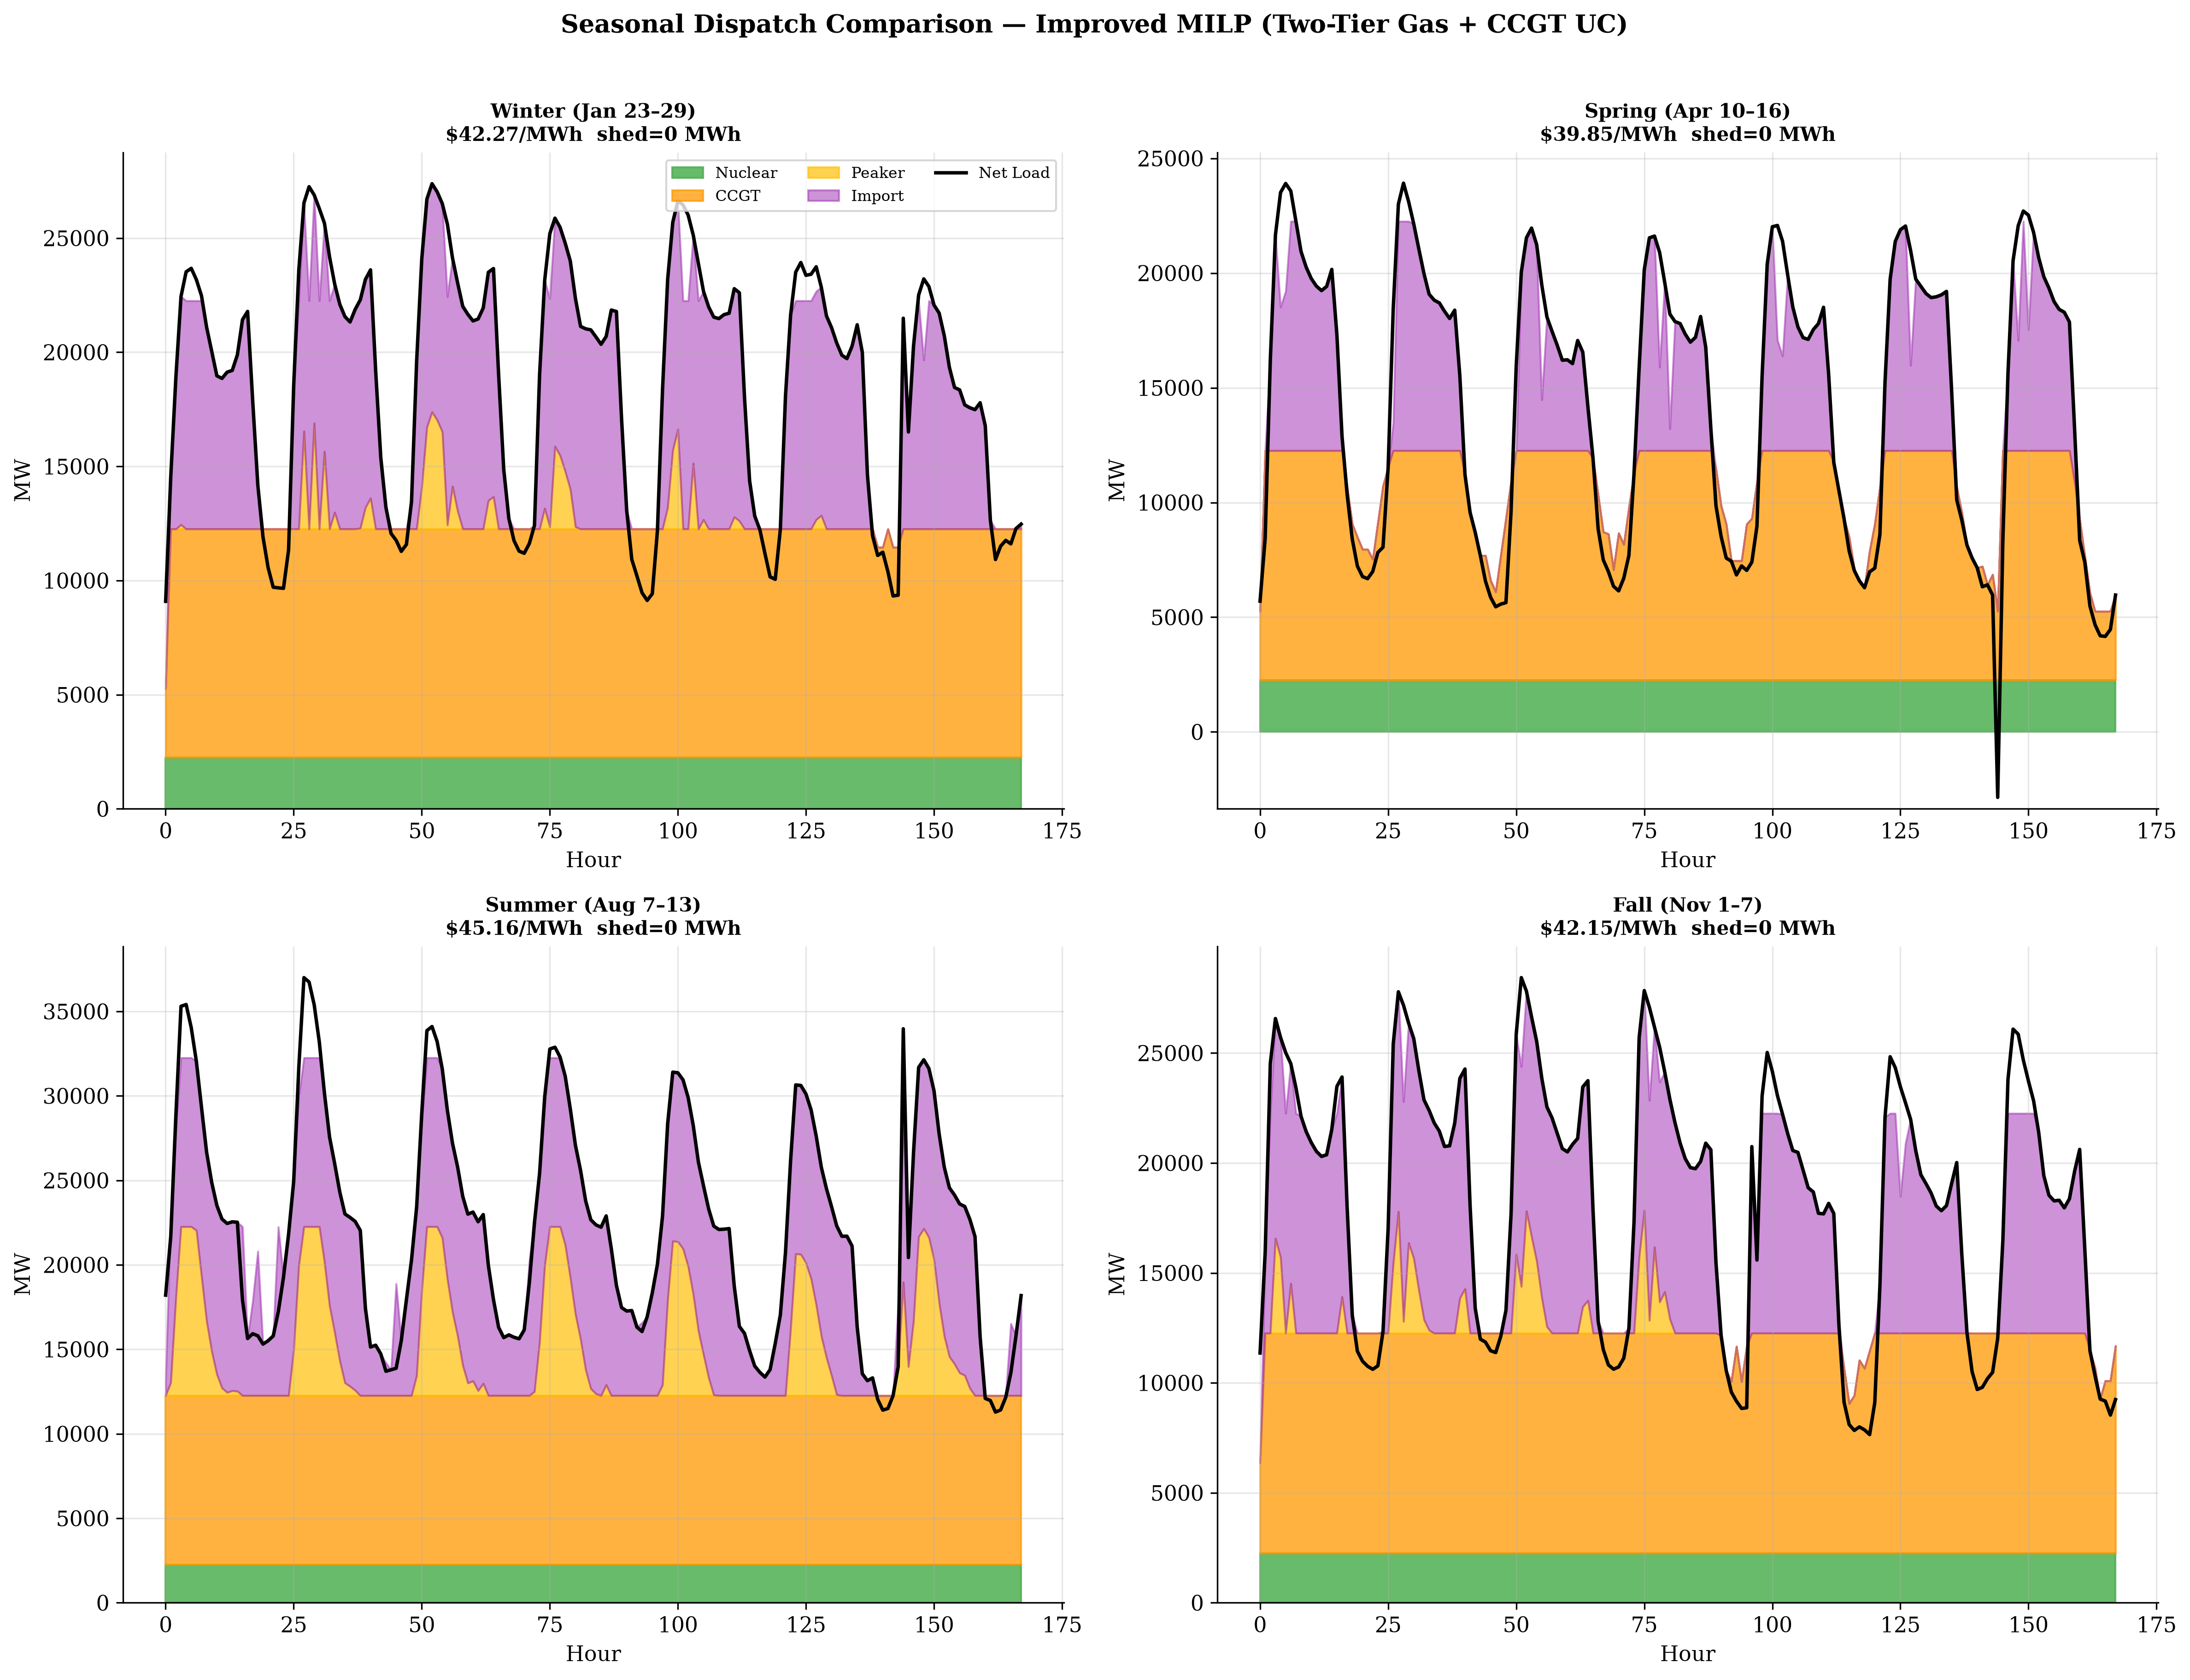
\includegraphics[width=\textwidth]{fig_seasonal_dispatch.png}
\caption{Four-season dispatch stacks (realized net load). Costs range from \$39.85/MWh (spring) to \$45.16/MWh (summer); zero load shedding in all seasons with nuclear online.}
\label{fig:seasons}
\end{figure}

\subsection{Value of Perfect Information}
\label{sec:vopi}

To quantify the economic cost of forecast uncertainty, we compare the day-ahead \emph{planning} cost under XGBoost predictions against an oracle plan using realized net load for the November week (forecast MAE for this week: 1{,}080~MW): \$41.84 vs.\ \$42.15/MWh, an absolute gap of \$0.31/MWh (0.74\%). We emphasize that this is a planning-stage comparison, not a realized-cost comparison: the ML forecast under-predicts mean net load by 570~MW, so its cheaper plan embeds an under-procurement whose real-time balancing cost is outside this single-stage model, and the \$0.31/MWh gap should be read as the order of magnitude of forecast-driven cost distortion rather than a strict VOPI bound. Even under this caveat, the gap is an order of magnitude below the nuclear premium (\$5.51/MWh), well within CAISO's typical balancing budget. Because the single representative week used here mixes a per-MWh cost gap with two different total-dispatch bases (oracle vs.\ ML net load), a robust annualized dollar figure requires a full two-settlement (day-ahead plus real-time recourse) evaluation across representative weeks, which we identify as future work.

\subsection{Sensitivity Analysis}
\label{sec:sensitivity}

Fig.~\ref{fig:sensitivity} presents three parametric sweeps (all with the two-tier UC model).

\begin{figure}[htbp]
\centering
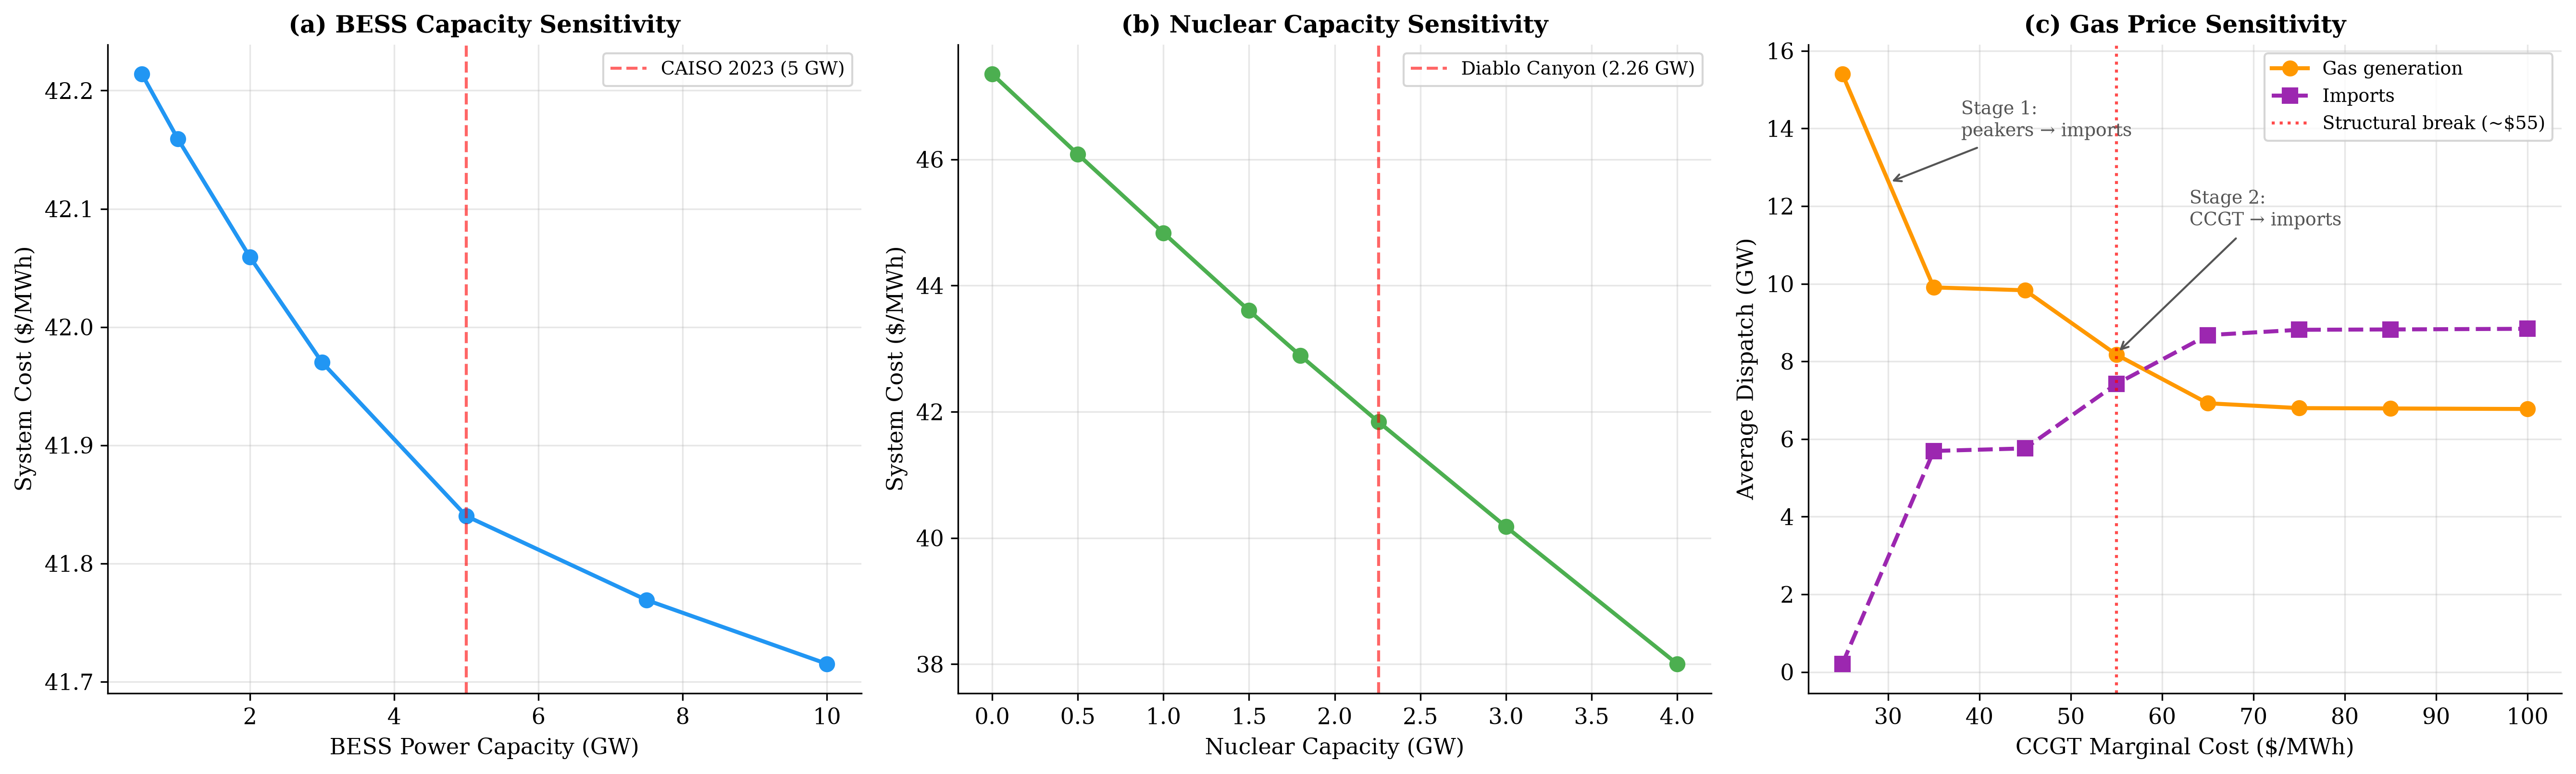
\includegraphics[width=\textwidth]{fig15_sensitivity_analysis.png}
\caption{Parametric sensitivity: (a) BESS capacity (0.5--10~GW), (b) nuclear capacity (0--4~GW), (c) gas price (\$25--\$100/MWh CCGT marginal cost) showing gas--import substitution.}
\label{fig:sensitivity}
\end{figure}

\textbf{Nuclear capacity (0--4~GW).} System cost declines nearly linearly at ${\sim}\$2.3$/MWh per GW: from \$47.35/MWh (0~GW) through \$41.84 (current 2.26~GW) to \$38.00 (4~GW). The two-tier model shows nuclear removal is backfilled by near-maximal CCGT output plus increasingly expensive peakers, the mechanism behind the higher premium relative to single-tier formulations.

\textbf{BESS sizing (0.5--10~GW).} BESS shows pronounced diminishing returns: 0.5 $\to$ 5~GW saves \$0.37/MWh, while 5 $\to$ 10~GW yields only a further \$0.13/MWh saving. Weekly cycling falls from 5.18 equivalent cycles (power-limited small systems) to 2.81 at 10~GW as marginal arbitrage saturates. CAISO's current 5~GW captures most available weekly arbitrage value.

\textbf{Gas price (\$25--\$100/MWh).} The sweep range spans the CCGT marginal costs implied by Henry Hub prices from the 2020 lows to the 2021--2022 stress period. The two-tier model reveals a two-stage substitution against the \$55/MWh import price. Around \$30/MWh CCGT cost, peakers (priced \$25/MWh above CCGT) lose to imports, dropping average gas from 15{,}402~MW (\$25) to 9{,}905~MW (\$35). The main structural break occurs near \$55/MWh, when CCGTs themselves lose merit order: average gas falls from 9{,}831~MW (\$45) to 6{,}921~MW (\$65) and plateaus near 6{,}800~MW, sustained by hours in which the 10~GW import limit binds. A carbon price of ${\sim}\$40$/tCO$_2$ (raising effective CCGT cost from ${\sim}\$40$ to ${\sim}\$55$/MWh at 0.37~t/MWh) would trigger this shift, displacing emissions accounting to neighboring balancing areas rather than eliminating them (carbon leakage).

\textbf{Import price (\$45--\$70/MWh).} Because gas--import substitution is central to the dispatch economics, we verify that the headline nuclear premium is not an artifact of the \$55/MWh import assumption: sweeping the import price from \$45 to \$70/MWh moves the S4$-$S1 premium only from $+12.7\%$ to $+14.1\%$ (Appendix Table~\ref{tab:impsens} and Fig.~\ref{fig:impsens}), with zero shedding throughout. The nuclear valuation is thus robust to the least certain exogenous price in the model.

\subsection{Robustness Parameter and Emissions}
\label{sec:gamma}

Sweeping $\gamma \in [0,1]$ (Table~\ref{tab:gamma}, Fig.~\ref{fig:pareto}) shows a nearly linear cost response: each 0.25 increment adds ${\sim}\$0.44$/MWh ($+1.0\%$), driven entirely by pre-scheduled additional gas. At $\gamma = 0.5$ the premium is \$0.79/MWh ($+1.9\%$) for protection up to the CQR 90th percentile; zero shedding at all $\gamma$ confirms capacity adequacy across the full CQR uncertainty range. The sweep exactly recovers S1, S6, and S2, confirming internal consistency.

Robustness also carries an emissions cost: weekly CO$_2$ rises monotonically from 1{,}029~kt ($\gamma{=}0$) to 1{,}254~kt ($\gamma{=}1$), a $+21.8\%$ emissions increase for a $+4.2\%$ cost increase. This cost--robustness--emissions tradeoff implies that more conservative dispatch is simultaneously more expensive and more carbon-intensive; because the hedging volume is $\gamma\,[\hat{q}_{0.90}(t) - \hat{P}(t)]$, a sharper forecast that narrows the calibrated interval directly shrinks the pre-scheduled fossil add-on at any given $\gamma$, making forecast quality an emissions-abatement lever, not merely an economic one. Scenario-level accounting (Appendix Fig.~\ref{fig:co2}) further shows nuclear removal raises weekly emissions from 1{,}029 to 1{,}207~kt ($+17.3\%$), i.e., ${\sim}9.3$~Mt~CO$_2$/year avoided by the 2.26~GW fleet at the modeled gas/import margin, above average-mix estimates (${\sim}7$~Mt) because displacement occurs at the fossil margin.

\begin{table}[htbp]
\centering
\caption{Robustness sweep (November week). $\gamma{=}0$ recovers S1; $\gamma{=}0.5$ recovers S6; $\gamma{=}1$ recovers S2.}
\label{tab:gamma}
\small
\resizebox{\textwidth}{!}{%
\begin{tabular}{lrrrrl}
\toprule
$\boldsymbol{\gamma}$ & \textbf{\$/MWh} & \textbf{Shed (MWh)} & \textbf{Avg gas (MW)} & \textbf{CO$_2$ (kt/wk)} & \textbf{Premium vs.\ $\gamma{=}0$} \\
\midrule
0.00 & 41.84 & 0 & 9{,}878  & 1{,}029 & --- \\
0.25 & 42.20 & 0 & 10{,}243 & 1{,}083 & $+\$0.36$ ($+0.9\%$) \\
0.50 & 42.63 & 0 & 10{,}629 & 1{,}139 & $+\$0.79$ ($+1.9\%$) \\
0.75 & 43.10 & 0 & 11{,}006 & 1{,}197 & $+\$1.26$ ($+3.0\%$) \\
1.00 & 43.59 & 0 & 11{,}275 & 1{,}254 & $+\$1.75$ ($+4.2\%$) \\
\bottomrule
\end{tabular}}
\end{table}

\begin{figure}[htbp]
\centering
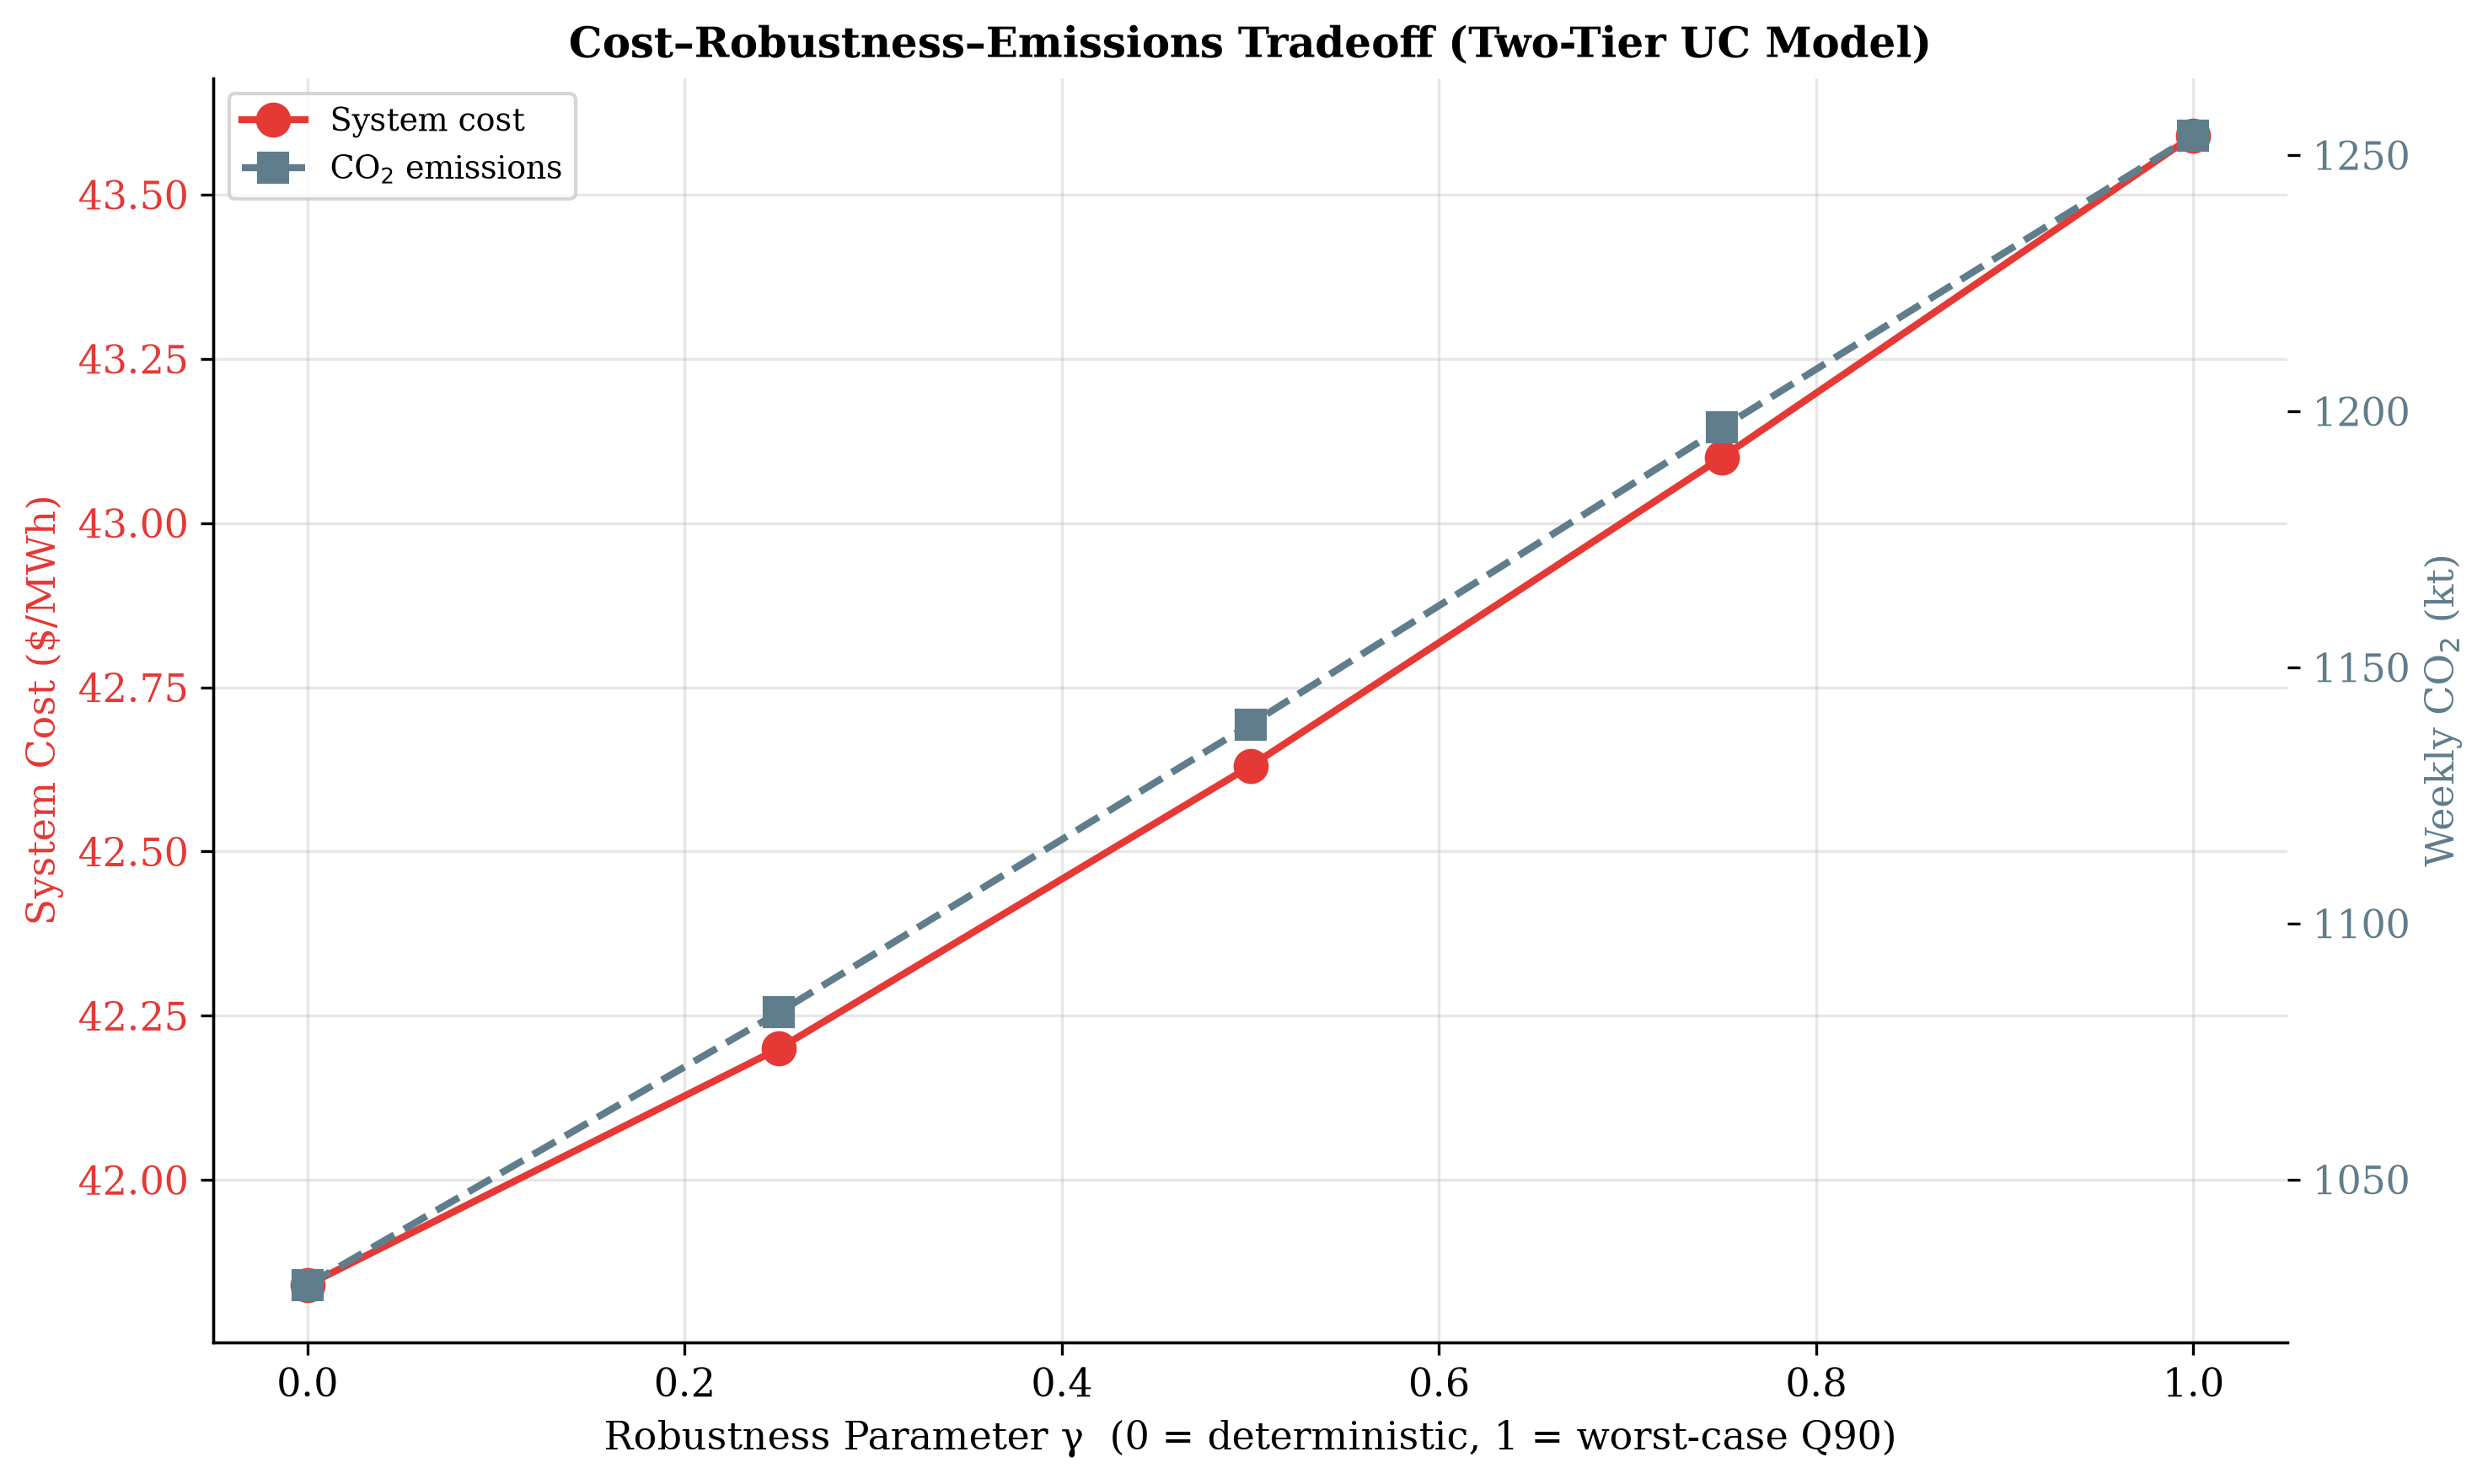
\includegraphics[width=0.85\textwidth]{fig_robust_pareto.png}
\caption{Cost--robustness--emissions tradeoff: system cost (left axis) and weekly CO$_2$ (right axis) vs.\ blending parameter $\gamma$.}
\label{fig:pareto}
\end{figure}

\subsection{Comparison with Two-Stage Stochastic Programming}
\label{sec:sp}

Table~\ref{tab:sp} benchmarks the CQR-robust approach against the two-stage SP baseline of Section~\ref{sec:milp} under the identical information set and out-of-sample protocol. Three observations stand out. First, the SP planning cost (\$42.04/MWh) sits between $\gamma = 0$ and $\gamma = 0.5$, i.e., the probability-weighted scenario tree implies a conservatism level of roughly $\gamma \approx 0.13$ (by linear interpolation between the $\gamma = 0$ and $\gamma = 0.5$ planning costs). Second, and most importantly, \emph{realized} costs against the actual net load are statistically indistinguishable across all four plans (\$42.15--\$42.16/MWh, zero shedding): because CAISO's recourse flexibility (CCGT output range, peakers, BESS, imports) is ample in the studied week, the first-stage commitment differences wash out in operation. Third, the SP achieves this equivalence at a higher price: it requires scenario probability assignments (which CQR avoids by construction), enlarges the model by 40\% in binary variables (1{,}176 vs.\ 840), and solves nearly three times slower (1.2~s vs.\ 0.4~s; wall-clock solve time is hardware-dependent, but the SP model consistently solves several-fold slower across repeated runs), a gap that compounds rapidly as scenario trees grow. We conclude that the CQR-robust formulation attains SP-level operational performance with a distribution-free coverage guarantee, a lighter model, and a transparent one-parameter conservatism dial; conversely, in systems with scarcer recourse flexibility, the plan-stage differences between the paradigms would be expected to re-emerge, a comparison we flag for future work.

\begin{table}[htbp]
\centering
\caption{CQR-robust vs.\ two-stage stochastic programming under the same information set (November week). Realized costs from frozen first-stage decisions re-dispatched against actual net load.}
\label{tab:sp}
\small
\resizebox{\textwidth}{!}{%
\begin{tabular}{lrrrrr}
\toprule
\textbf{Plan} & \textbf{Planning (\$/MWh)} & \textbf{Realized (\$/MWh)} & \textbf{Shed (MWh)} & \textbf{Binaries} & \textbf{Solve (s)} \\
\midrule
Deterministic ($\gamma{=}0$) & 41.84 & 42.15 & 0 & 840   & 0.43 \\
Robust ($\gamma{=}0.5$)      & 42.63 & 42.16 & 0 & 840   & 0.42 \\
Robust ($\gamma{=}1$, Q90)   & 43.59 & 42.16 & 0 & 840   & 0.30 \\
SP (3-scenario, Swanson--Megill) & 42.04 & 42.15 & 0 & 1{,}176 & 1.17 \\
\bottomrule
\end{tabular}}
\end{table}

\subsection{Annual Robustness of the Nuclear Premium (50-Week Sweep)}
\label{sec:fullyear}

The single-week scenarios of Section~\ref{sec:results_milp} raise an obvious question: is the November week representative? To test this, we solve the improved MILP, with and without nuclear, for every one of the 50 non-overlapping 168-hour windows spanning the full realized 2023 net load record (January~8 to December~31; each window re-initializes SoC at 50\%, so weeks are independent, self-contained dispatch problems), yielding 100 additional MILP solves at $< 1$~s each.

Two regimes emerge cleanly (Fig.~\ref{fig:fullyear}). In 35 of 50 weeks (70\%, all outside late June--mid September), net load stays within the stylized fleet's capacity envelope and the nuclear premium is tightly clustered at $11.7$--$15.0\%$ (mean $13.45\%$, median $13.4\%$), directly validating the representativeness of the November baseline ($+13.2\%$). In the remaining 15 weeks, concentrated in a summer heat cluster plus two isolated events, net load approaches or exceeds the fleet's aggregate capacity and the premium diverges sharply, averaging $+74\%$ and peaking at $+210\%$ in the week of July~16--22, which contains the annual net load maximum (44{,}900~MW), a week that lies outside the four typical seasonal sample weeks of Section~\ref{sec:results_seasonal}.

This divergence must be interpreted with an important caveat: in 11 of these 15 weeks, load shedding occurs even \emph{with} nuclear online, which the stylized fleet (2{,}256~MW nuclear, 20~GW two-tier gas, 5~GW/20~GWh BESS, 10~GW imports) cannot fully resolve. This is a modeling artifact, not a reproduction of observed CAISO reliability outcomes: the fleet omits CAISO's actual hydroelectric and pumped-storage capacity (${\sim}6$--$8$~GW), demand response programs, and out-of-market emergency measures, all of which the real system deployed during the July--September 2023 heat events without resorting to rotating outages \citep{caiso2023}. The correct reading is therefore not ``CAISO nearly lost load in 2023,'' but that nuclear's \emph{reliability} value, distinct from and additive to its ${\sim}13\%$ economic value, rises sharply as a stylized capacity-constrained system approaches its frontier, consistent with the capacity-adequacy literature \citep{sepulveda2018}. Reassuringly, the full-year CO$_2$ saving from nuclear (${\sim}9.0$~Mt/year, summed over 50 weeks) closely matches the single-week extrapolation (${\sim}9.3$~Mt/year, Section~\ref{sec:gamma}), cross-validating both estimates.

\begin{figure}[htbp]
\centering
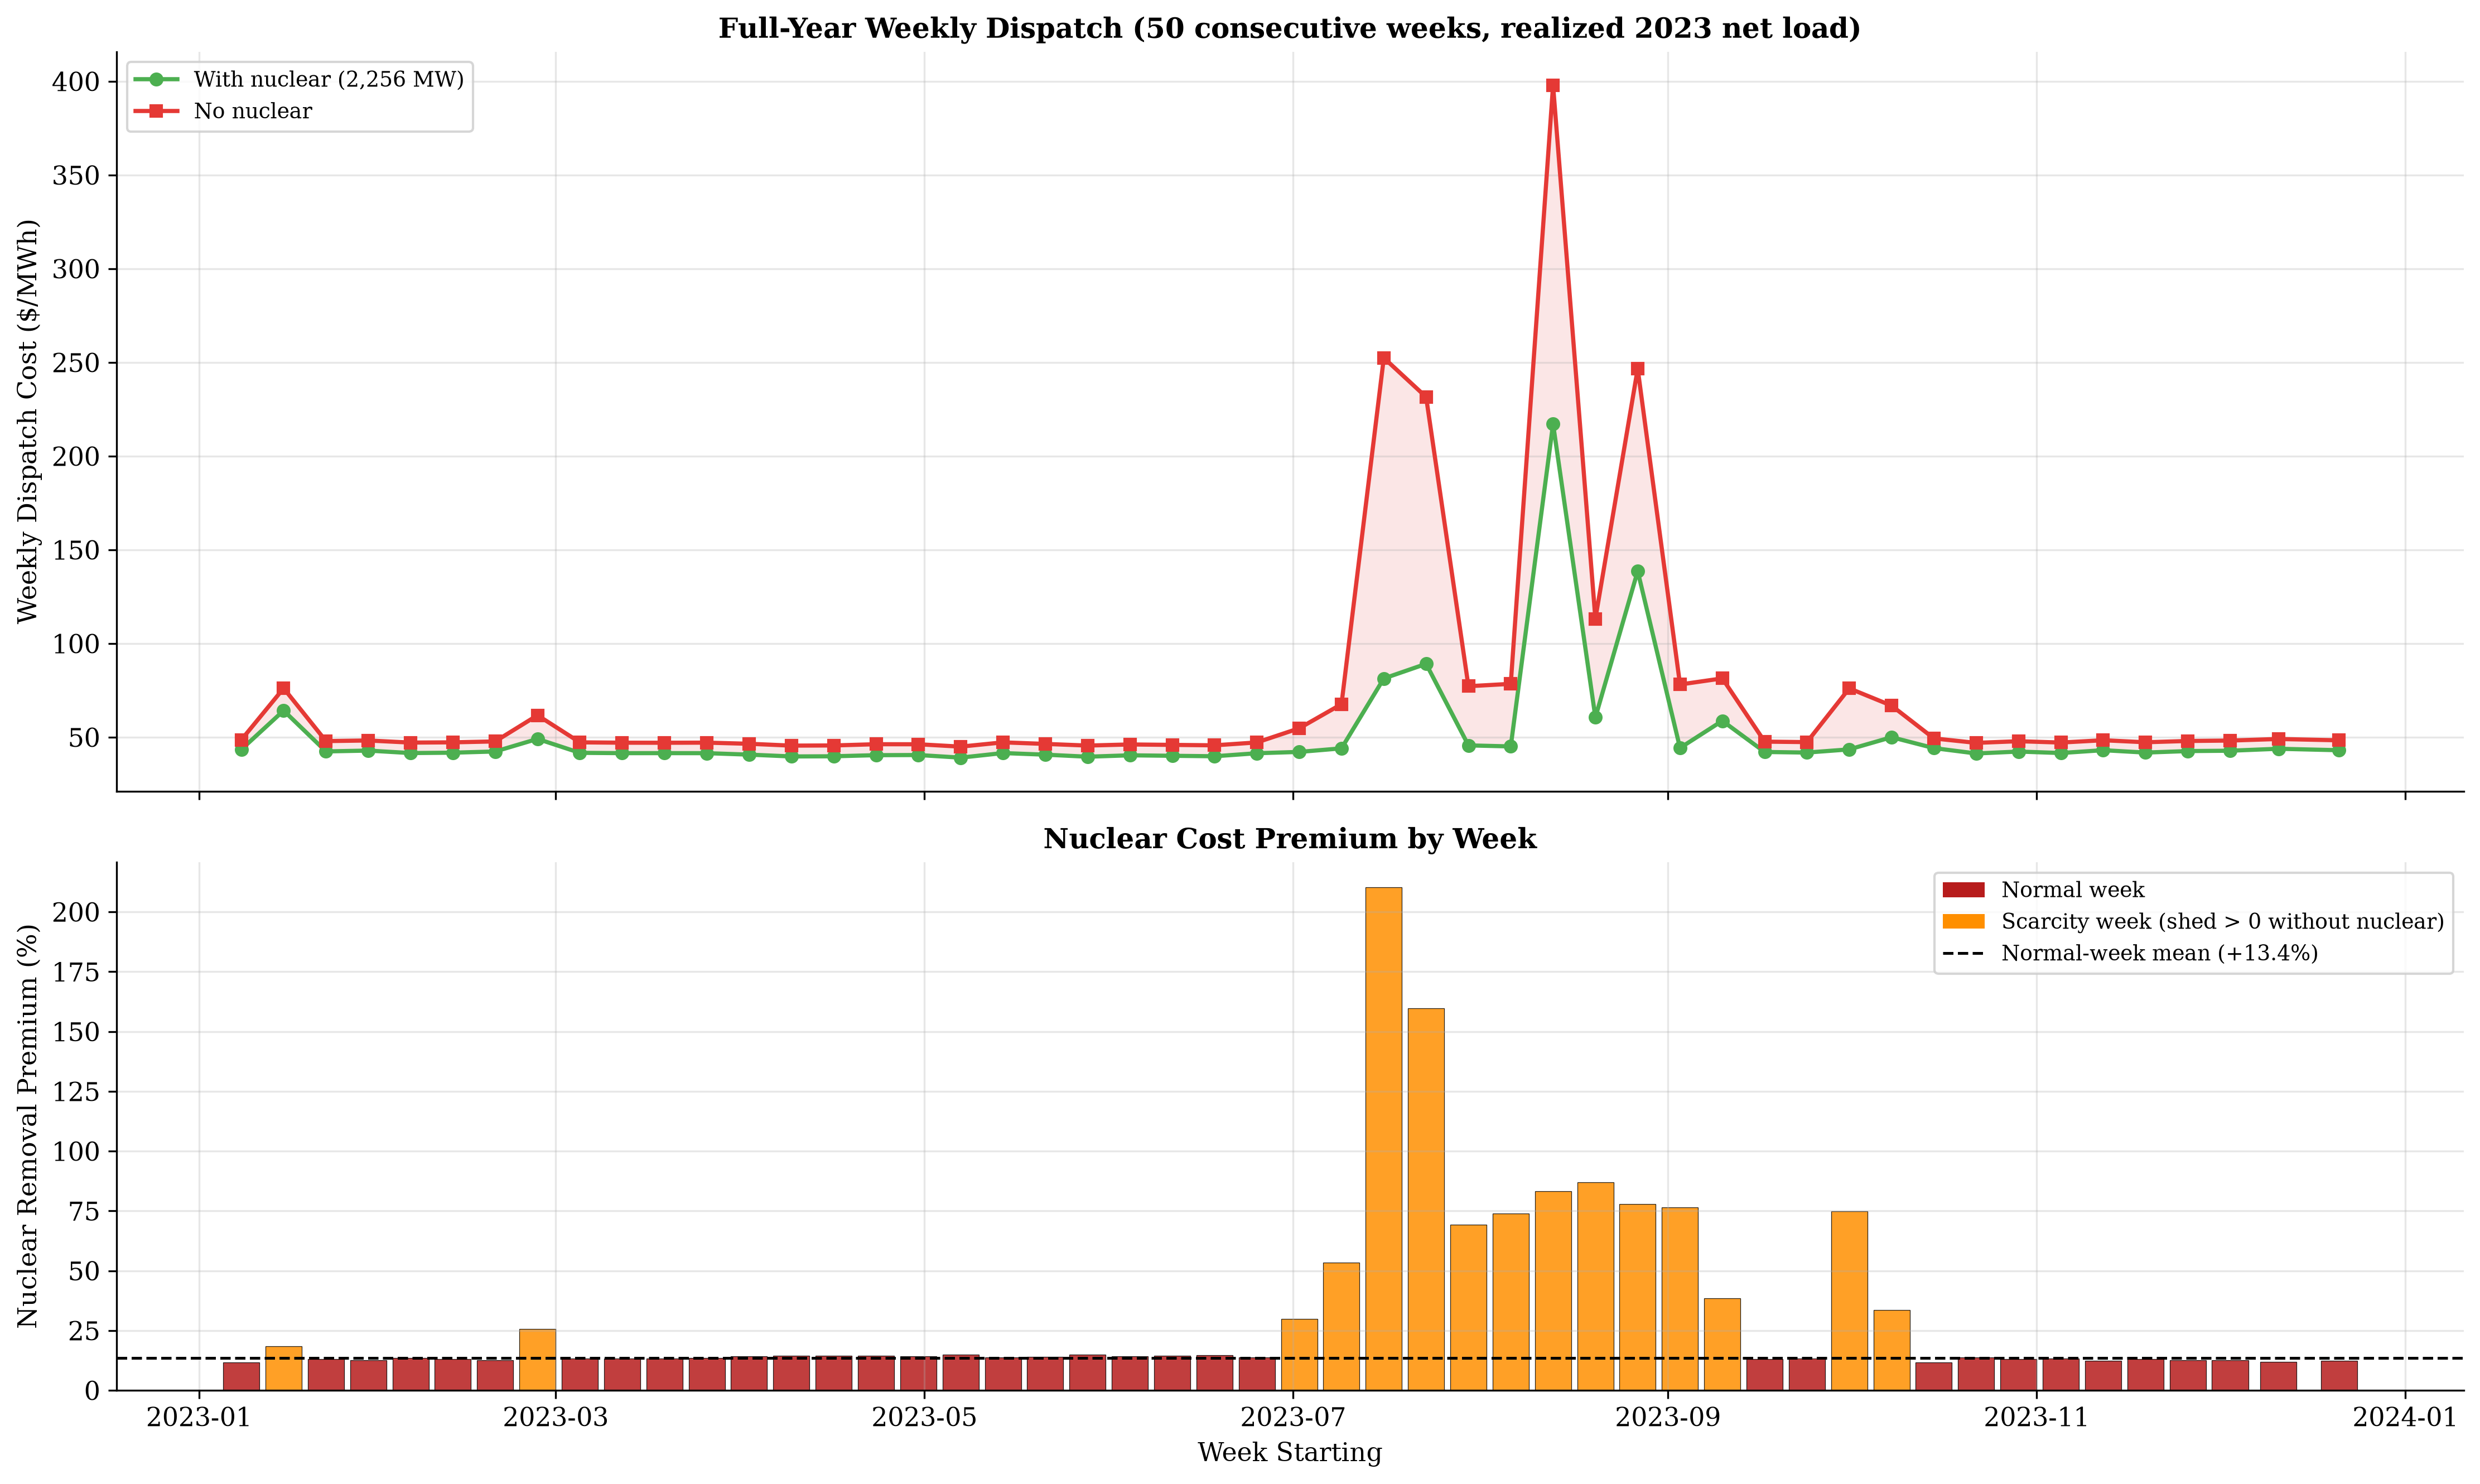
\includegraphics[width=\textwidth]{fig_fullyear_dispatch.png}
\caption{Full-year weekly dispatch (50 consecutive weeks, realized 2023 net load). Top: dispatch cost with and without nuclear. Bottom: nuclear removal premium, colored by regime: normal weeks (dark red, tightly clustered near the November baseline) vs.\ scarcity weeks (orange, shed $>0$ without nuclear, concentrated in summer).}
\label{fig:fullyear}
\end{figure}

\textbf{Validating the modeling-artifact interpretation with realized hydro.} Rather than merely assert that the summer shedding above is an artifact of the omitted hydro fleet, we test it directly: the 15 scarcity weeks are re-solved (with nuclear) after adding realized 2023 hourly CAISO hydroelectric generation (EIA Form~930 fuel-type series, Section~\ref{sec:data}) as an additional must-take resource, dispatched ahead of thermal generation, consistent with the largely run-of-river, environmentally constrained operation of CAISO hydro; although CAISO's fleet also includes dispatchable storage hydro, treating realized output as must-take is a conservative lower bound on hydro's flexibility contribution. This requires no change to the core MILP; it only supplies the historical hydro profile the stylized fleet omits. The result strongly confirms the artifact interpretation (Table~\ref{tab:hydro}, Fig.~\ref{fig:hydro}): total shedding across the 15 weeks falls by $93.4\%$ (from 167{,}506 to 11{,}021~MWh), and 11 of 15 weeks are fully resolved to zero shedding. The four weeks retaining residual shedding (January~15, February~26, July~16, September~10) are consistent with the one remaining omitted resource, demand response, which CAISO also deployed during 2023 stress events but which is not modeled here. This quantifies, rather than merely asserts, that the scarcity-week shedding predominantly reflects the stylized fleet's missing hydro capacity rather than a genuine CAISO reliability shortfall.

\begin{table}[htbp]
\centering
\caption{Effect of realized 2023 CAISO hydro generation on the 15 flagged scarcity weeks (with nuclear online).}
\label{tab:hydro}
\small
\begin{tabular}{lr}
\toprule
\textbf{Metric} & \textbf{Value} \\
\midrule
Total shedding without hydro & 167{,}506~MWh \\
Total shedding with realized hydro added & 11{,}021~MWh \\
Reduction in total shedding & $93.4\%$ \\
Weeks fully resolved (zero shedding) & 11 / 15 \\
\bottomrule
\end{tabular}
\end{table}

\begin{figure}[htbp]
\centering
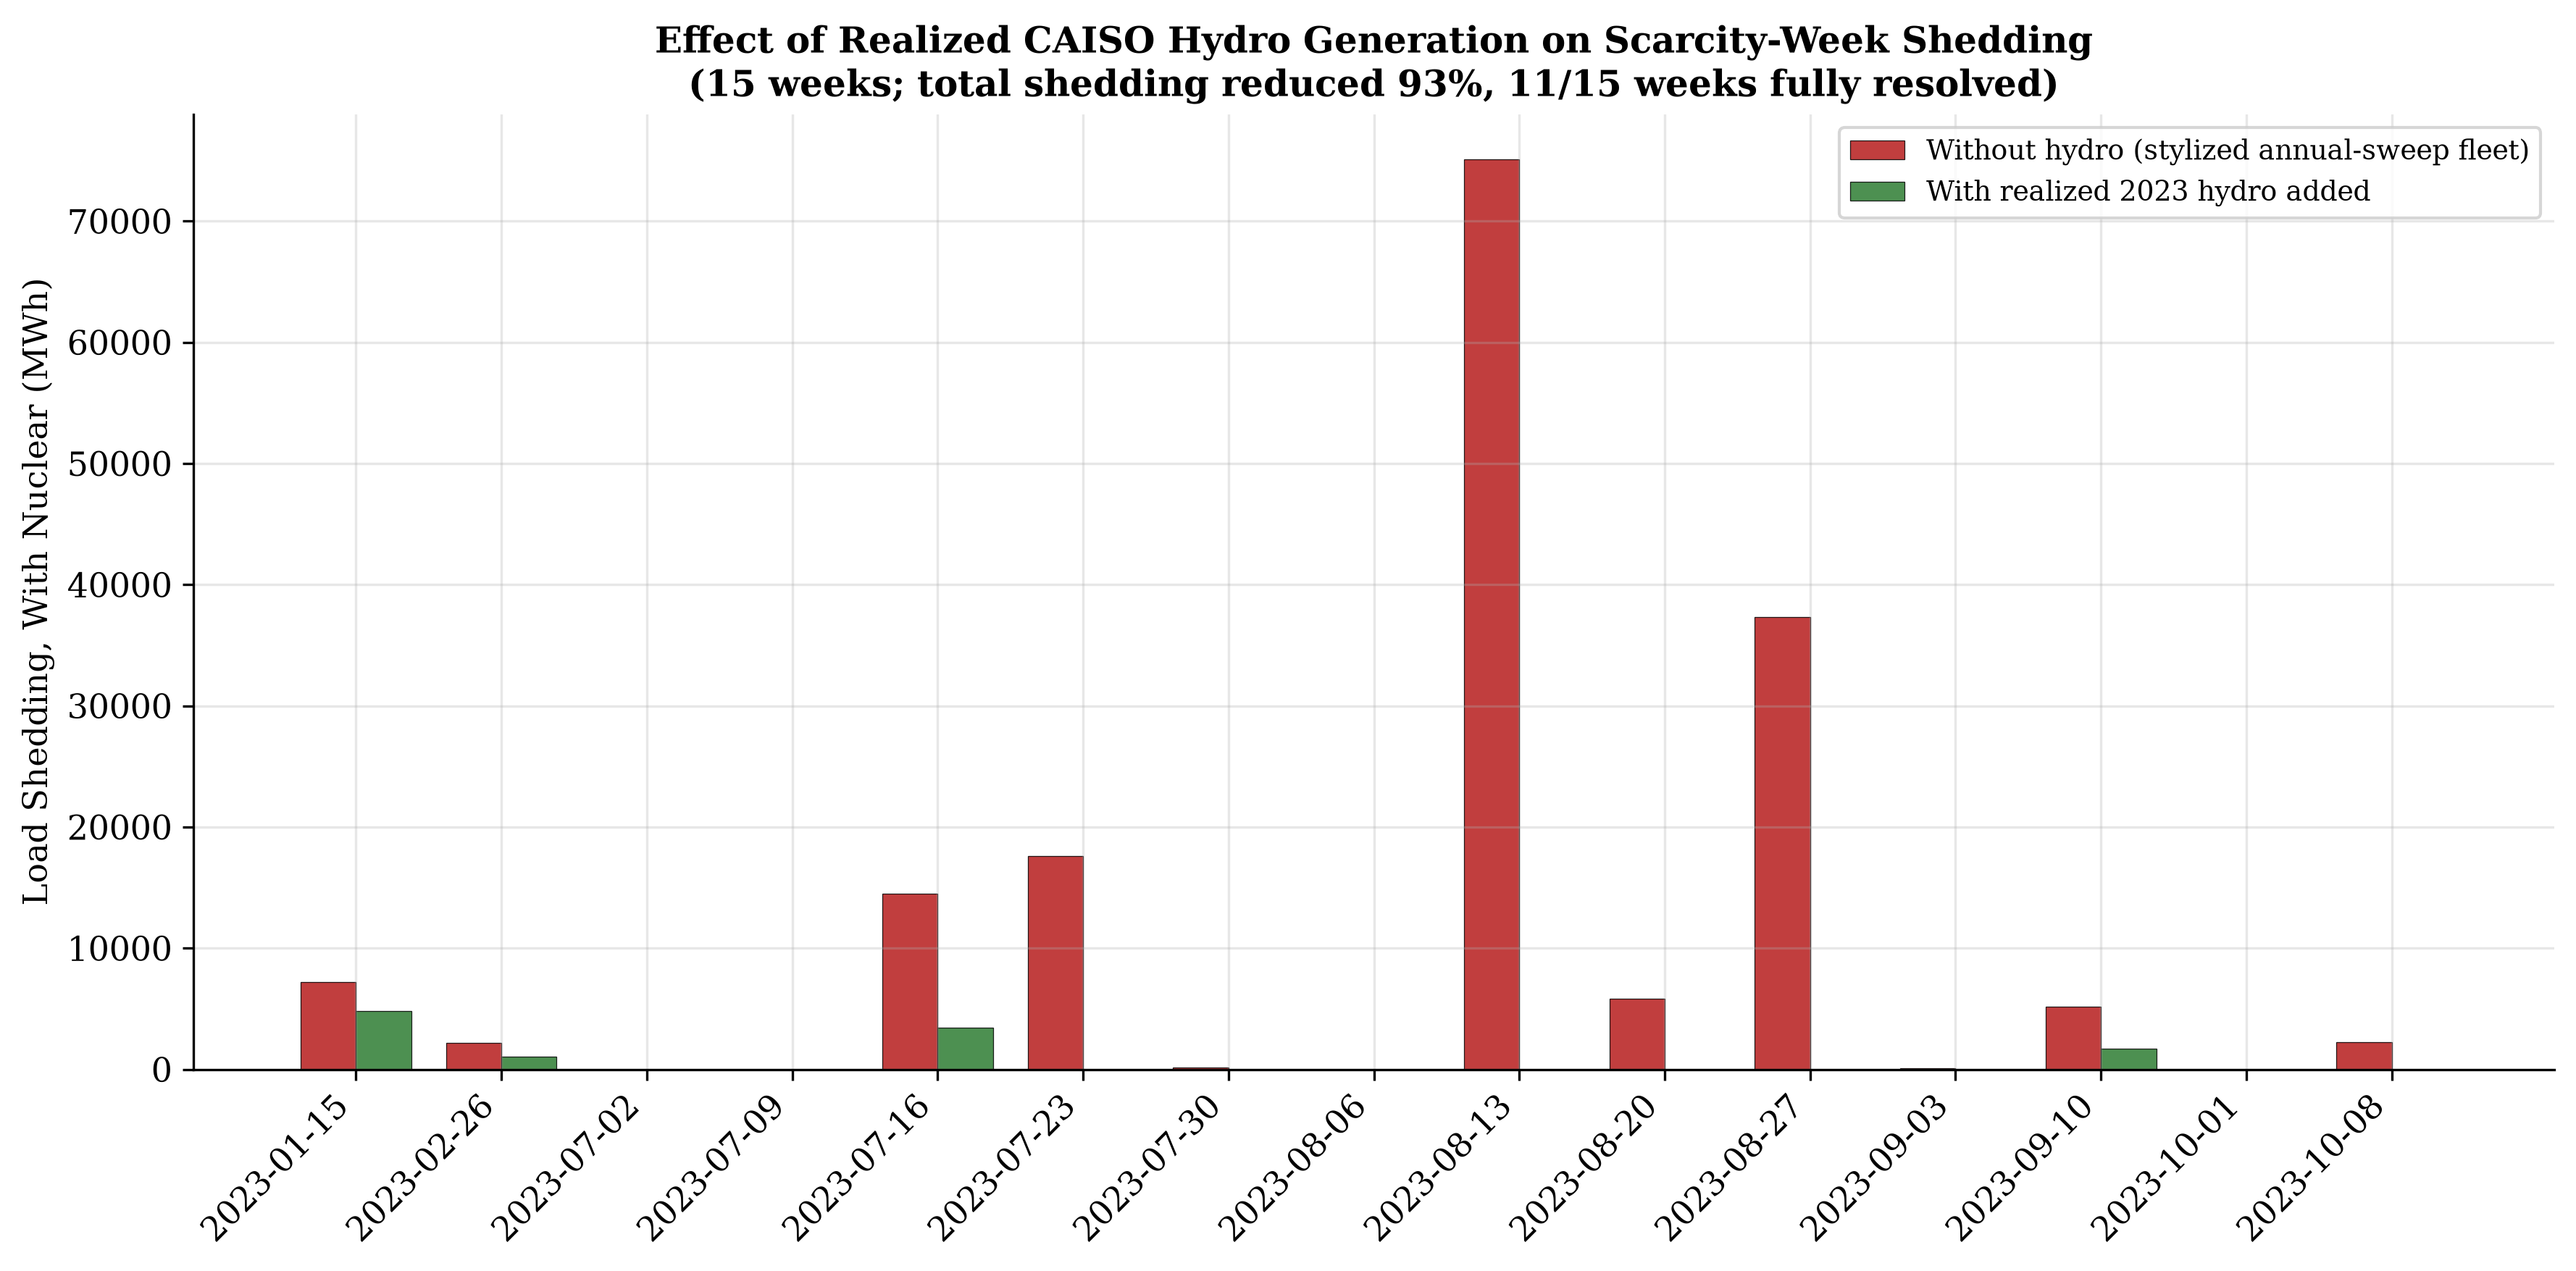
\includegraphics[width=\textwidth]{fig_hydro_robustness.png}
\caption{Effect of adding realized 2023 CAISO hydro generation (must-take, dispatched ahead of thermal) on load shedding in the 15 scarcity weeks, with nuclear online. Total shedding falls by 93\%; 11 of 15 weeks are fully resolved to zero.}
\label{fig:hydro}
\end{figure}

\subsection{Supplementary Check: Directional Transferability Beyond CAISO}
\label{sec:ercot}

The 50-week sweep establishes representativeness \emph{within} CAISO; a natural follow-up question is whether the same scarce-recourse mechanism operates in other grids. We do not attempt a second full case study, since that would require officially sourced unit-level capacity data and a full annual sweep beyond this paper's scope, but run a narrowly framed supplementary check: the identical MILP code, re-parameterized with illustrative ERCOT-like fleet and import-capacity values, applied to two non-extreme 2023 weeks (\ref{app:ercot} gives the full parameterization, table, and figure). The result is directionally consistent with the paper's central scarce-recourse mechanism: with island-grid import capacity an order of magnitude below CAISO's (1.22~GW vs.\ 10~GW), the nuclear premium is larger ($+14.9\%$ and $+15.8\%$) than the CAISO baseline ($+13.2\%$). We report this strictly as a qualitative transferability signal rather than a calibrated regional estimate, given the illustrative parameterization and the two-week scope; a rigorously sourced, full-year study of another grid is identified as future work (Section~\ref{sec:conclusion}).


%% ====================================================================
\section{Discussion}
\label{sec:discussion}
%% ====================================================================

\subsection{Policy Implications}

Nuclear baseload value in CAISO is primarily \emph{economic} under typical operating conditions: the no-nuclear dispatch maintains zero shedding in all four representative seasonal weeks, but at a sustained \$5.51/MWh premium and $+17.3\%$ emissions. This economic-value characterization does not extend to capacity-stress conditions: the 50-week annual sweep (Section~\ref{sec:fullyear}) shows that during summer weeks approaching the system's capacity frontier, nuclear's \emph{reliability} value becomes dominant, with the premium rising to $+74\%$ on average and $+210\%$ at the annual net load peak, a second, distinct value stream additive to the baseline economic premium. We stress that this is an \emph{operating-cost} estimate under fixed technology prices, not a market-equilibrium one: removing 2.26~GW of baseload would in reality shift wholesale prices and import flows, effects a price-taking dispatch model cannot capture. The premium is nonetheless robust to the least certain of those prices (import cost; $+12.7$ to $+14.1\%$ over \$45--\$70/MWh, Section~\ref{sec:sensitivity}). At \$2.3/MWh per GW across the 0--4~GW range, nuclear provides consistent marginal value that supports its retention as low-cost zero-carbon baseload, strongest in high-demand periods when peaker and import costs bind. The planning-stage VOPI of \$0.31/MWh suggests forecast uncertainty is not the binding constraint on system economics (subject to the single-stage caveat of Section~\ref{sec:vopi}); the CQR robustness lever $\gamma$ is cheap insurance ($+1.0\%$ cost per 0.25 increment) but carries a disproportionate emissions premium, which operators and regulators should weigh jointly. The ${\sim}\$40$/tCO$_2$ gas--import substitution threshold cautions that carbon pricing in one balancing area can induce leakage through imports.

\subsection{Comparison with Prior Literature}

Our day-ahead net load skill ($+18.5\%$ over persistence) is consistent with, and slightly above, the 10--15\% gains reported in load forecasting competitions \citep{hong2016,hong2020review}, reflecting the greater variability of the net load target. The GBM-over-deep-learning result matches benchmark findings on moderate-scale tabular data \citep{hertel2022,grinsztajn2022}. CQR coverage (88.8\% vs.\ 90\% target) aligns with \citet{romano2019}. Our nuclear value (\$2.3/MWh per GW) falls at the lower end of \citet{jenkins2018} estimates for generic U.S.\ systems, consistent with CAISO's large gas fleet and import capacity providing alternative flexibility, and with the firm-resource value identified by \citet{sepulveda2018}. The gas-price tipping point echoes \citet{bistline2023} but is derived from actual 2023 operational data rather than capacity-expansion models.

\subsection{Limitations}

Six main limitations apply. (i)~\emph{Copper-plate network}: transmission is omitted; the two-zone Path~15 extension bounds the aggregate cost effect at $+3.7\%$ and scenario comparisons difference it out, but nodal congestion rents remain unquantified. (ii)~\emph{Aggregate CCGT fleet}: two 5{,}000~MW units approximate ${\sim}200$ physical units; the \$25{,}000/event startup cost reflects warm starts (\citealp{nrelatb2023}), conservatively below cold-start estimates. We tested sensitivity to this choice directly: re-solving S1 and S4 with four 2{,}500~MW units instead of two 5{,}000~MW units (same 10~GW total capacity, minimum-load fraction, and per-unit ramp rate) changes the nuclear premium by only $0.01$ percentage points ($13.175\%$ vs.\ $13.165\%$), confirming the headline results are insensitive to this aggregation choice; individual unit commitment would still improve fidelity for maintenance scheduling and heat-rate curves. (iii)~\emph{CQR exchangeability and conditional coverage}: time series dependence technically violates exchangeability, and while marginal coverage is near-nominal, hour-conditional coverage drops to ${\sim}79\%$ during evening ramps (Fig.~\ref{fig:confdiag}); adaptive and Mondrian-style conformal methods \citep{gibbs2021,zaffran2022} would address both issues. (iv)~\emph{Single-stage, single-year scope}: the MILP is day-ahead only (no real-time recourse stage) and uses 2023 conditions; multi-year analysis would capture secular VRE growth. (v)~\emph{Import representation}: imports are modeled at a constant \$55/MWh with 10~GW availability; during West-wide stress events (e.g., regional heat waves), both the price and the availability of imports deteriorate simultaneously, so the no-nuclear scenarios likely \emph{understate} scarcity costs, and our nuclear valuation is conservative in this respect. (vi)~\emph{Stylized capacity envelope and ERCOT parameterization}: the fleet used in the annual sweep (Section~\ref{sec:fullyear}) omits CAISO's hydroelectric, pumped-storage, and demand-response resources, causing artificial load shedding in some summer weeks that did not occur in reality. We tested this directly rather than merely disclosing it: adding realized 2023 hourly CAISO hydro generation as a must-take resource eliminates $93.4\%$ of the flagged shedding and fully resolves 11 of the 15 affected weeks (Table~\ref{tab:hydro}); the residual shedding in the remaining four weeks is consistent with demand response, the one omitted resource we could not similarly test with historical dispatch data. The supplementary ERCOT check (Section~\ref{sec:ercot}, \ref{app:ercot}) is deliberately scoped as a qualitative transferability signal, not a second case study: it uses illustrative, not officially sourced, fleet parameters over only two non-extreme weeks, and we report it strictly as evidence that the scarcity mechanism points in the expected direction outside CAISO, not as a calibrated ERCOT-specific policy estimate.


%% ====================================================================
\section{Conclusions}
\label{sec:conclusion}
%% ====================================================================

This study presents an integrated data-driven framework coupling conformalized quantile regression with robust MILP dispatch, applied to CAISO using real 2023 operational data. The key conclusions:

\begin{enumerate}
    \item \textbf{Forecasting.} XGBoost with 35 leakage-free features achieves $R^2 = 0.854$ and MAE = 1{,}429~MW day-ahead, $+18.5\%$ over persistence (DM $p < 0.001$), with the companion LightGBM configuration stable across seasons (CV $R^2 = 0.869 \pm 0.089$) and years (2022 out-of-sample $R^2 = 0.908$). Deep learning baselines underperform persistence at this data scale.

    \item \textbf{Calibrated uncertainty.} CQR delivers 88.8\% empirical coverage at a 90\% target with adaptive width (mean 5{,}182~MW), enabling distribution-free uncertainty propagation into optimization.

    \item \textbf{Nuclear value.} {\sloppy Removing 2.26~GW of nuclear raises system cost 13.2\% (\$41.84 $\to$ \$47.35/MWh) and weekly CO$_2$ emissions 17.3\% (${\sim}9.3$~Mt/year annualized at the fossil margin). Under typical conditions the value (\$2.3/MWh per GW, linear over 0--4~GW) is primarily economic: the gas fleet and imports maintain zero shedding, at a premium.\par}

    \item \textbf{Seasonal adequacy and VOPI.} Dispatch cost spans \$39.85 (spring) to \$45.16/MWh (summer) with zero shedding in all four representative seasonal weeks; the planning-stage value of perfect information is \$0.31/MWh (0.74\%), supporting the use of ML forecasts as MILP inputs subject to the two-settlement caveat of Section~\ref{sec:vopi}.

    \item \textbf{Tradeoffs.} A gas--import substitution break at ${\sim}\$55$/MWh CCGT cost (${\sim}\$40$/tCO$_2$ carbon price) raises carbon-leakage concerns, and robust dispatch is a cost--robustness--emissions tradeoff ($+4.2\%$ cost, $+21.8\%$ CO$_2$ at $\gamma{=}1$), making forecast quality itself an emissions lever.

    \item \textbf{CQR-robust vs.\ stochastic programming.} Under an identical information set and out-of-sample protocol, a two-stage SP baseline attains the same realized cost as the CQR-robust dispatch (\$42.15 vs.\ \$42.16/MWh, zero shedding) while requiring scenario probabilities, 40\% more binaries, and several-fold longer solves; the CQR-robust formulation delivers SP-level performance with a distribution-free guarantee and a lighter model.

    \item \textbf{Annual robustness and transferability.} A 50-week sweep of the full 2023 record confirms the November premium is representative of typical operation (13.45\% mean across 35 normal weeks) while revealing a second, reliability-driven regime during summer capacity-stress weeks (premium up to $+210\%$). Two targeted checks validate this finding rather than merely disclosing its limitations: adding realized 2023 CAISO hydro generation eliminates 93.4\% of the flagged shedding (11 of 15 weeks fully resolved), confirming a modeling-artifact rather than a genuine-reliability interpretation, and re-solving with four 2{,}500~MW CCGT units instead of two 5{,}000~MW units changes the nuclear premium by only 0.01 percentage points. A narrowly scoped supplementary check on an ERCOT-parameterized grid (\ref{app:ercot}) shows the same scarcity mechanism directionally amplifying the premium ($+15$--$16\%$) under an island grid's limited import capacity, a qualitative transferability signal, not a calibrated regional estimate.
\end{enumerate}

Future work includes nodal transmission modeling, multi-year horizons, weather-ensemble inputs to the CQR framework, adaptive conformal inference for non-stationarity, extending the optimization to demand response, electric vehicle charging, and hydrogen production as flexibility resources, a full capacity-adequacy representation of the CAISO fleet (hydroelectric, pumped storage, and demand response) to replace the stylized envelope used in the annual sweep, and a rigorously sourced, full-year ERCOT study using official CDR unit-level capacity data.

\section*{CRediT authorship contribution statement}
\textbf{Cagatay Kuban}: Conceptualization, Methodology, Software, Data curation, Formal analysis, Validation, Visualization, Writing -- original draft, Writing -- review \& editing.

\section*{Declaration of competing interest}
The author declares that they have no known competing financial interests or personal relationships that could have appeared to influence the work reported in this paper.

\section*{Data availability}
All data are publicly available from the U.S.\ Energy Information Administration (\url{https://api.eia.gov}) and NOAA (\url{https://www.ncei.noaa.gov}). Code and processed datasets are available from the corresponding author upon reasonable request.

\section*{Declaration of generative AI and AI-assisted technologies in the manuscript preparation process}
During the preparation of this work the author used the Claude Sonnet model (Anthropic) for language support and coding support. After using this tool, the author reviewed and edited the content as needed and takes full responsibility for the content of the published article.

%% ====================================================================
\appendix
\setcounter{table}{0}
\setcounter{figure}{0}
\section{Additional Tables and Figures}
\label{app:a}
%% ====================================================================

This appendix reports supporting diagnostics referenced from Sections~\ref{sec:results_cv} and~\ref{sec:results_pi}.

\textbf{Error diagnostics.} Formal residual tests (Table~\ref{tab:diag}) show left-skewed (skewness $-0.72$), non-Gaussian errors (Jarque--Bera and Shapiro--Wilk $p < 0.001$) with significant residual autocorrelation at 24 lags (Ljung--Box $p < 0.001$), expected for electricity data and immaterial for CQR, which is distribution-free; empirical coverage remains near-nominal. Hyperparameter sensitivity (Table~\ref{tab:hyper}) shows test $R^2$ varies by only 1.3 percentage points across an $8\times$ range of \texttt{num\_leaves}; the reported configuration (63 leaves) is selected on validation MAE, which it minimizes, confirming the selection is not test-set-driven despite \texttt{num\_leaves}$=31$ scoring marginally higher on the held-out test fold.

\begin{table}[htbp]
\centering
\caption{Error diagnostics for net load forecasting models (test set).}
\label{tab:diag}
\small
\resizebox{\textwidth}{!}{%
\begin{tabular}{lrrrrrr}
\toprule
\textbf{Model} & \textbf{Mean err.} & \textbf{Skew.} & \textbf{Kurt.} & \textbf{JB $p$} & \textbf{SW $p$} & \textbf{LB(24) $p$} \\
\midrule
LightGBM      & $-175$ & $-0.73$ & $-0.005$ & $<0.001$ & $<0.001$ & $<0.001$ \\
XGBoost       & $-143$ & $-0.72$ & $-0.007$ & $<0.001$ & $<0.001$ & $<0.001$ \\
Random Forest & $-161$ & $-0.73$ & $-0.004$ & $<0.001$ & $<0.001$ & $<0.001$ \\
\bottomrule
\end{tabular}}
\end{table}

\begin{table}[htbp]
\centering
\caption{Import price sensitivity of the nuclear premium (November week).}
\label{tab:impsens}
\small
\resizebox{\textwidth}{!}{%
\begin{tabular}{rrrrrr}
\toprule
\textbf{Import (\$/MWh)} & \textbf{S1 (\$/MWh)} & \textbf{S4 (\$/MWh)} & \textbf{Premium} & \textbf{S4 import (MW)} & \textbf{S4 shed (MWh)} \\
\midrule
45 & 38.61 & 43.52 & $+12.7\%$ & 7{,}050 & 0 \\
50 & 40.23 & 45.48 & $+13.1\%$ & 6{,}678 & 0 \\
55 & 41.84 & 47.35 & $+13.2\%$ & 6{,}678 & 0 \\
60 & 43.44 & 49.22 & $+13.3\%$ & 6{,}678 & 0 \\
65 & 45.03 & 51.10 & $+13.5\%$ & 4{,}148 & 0 \\
70 & 45.09 & 51.45 & $+14.1\%$ & 1{,}257 & 0 \\
\bottomrule
\end{tabular}}
\end{table}

\begin{table}[htbp]
\centering
\caption{Hyperparameter sensitivity (LightGBM, \texttt{num\_leaves}).}
\label{tab:hyper}
\small
\begin{tabular}{crrr}
\toprule
\texttt{num\_leaves} & \textbf{Val MAE (MW)} & \textbf{Test MAE (MW)} & \textbf{Test $R^2$} \\
\midrule
31  & 1{,}410 & 1{,}457 & 0.854 \\
63  & 1{,}365 & 1{,}565 & 0.843 \\
127 & 1{,}408 & 1{,}534 & 0.841 \\
255 & 1{,}408 & 1{,}534 & 0.841 \\
\bottomrule
\end{tabular}
\end{table}

\begin{figure}[htbp]
\centering
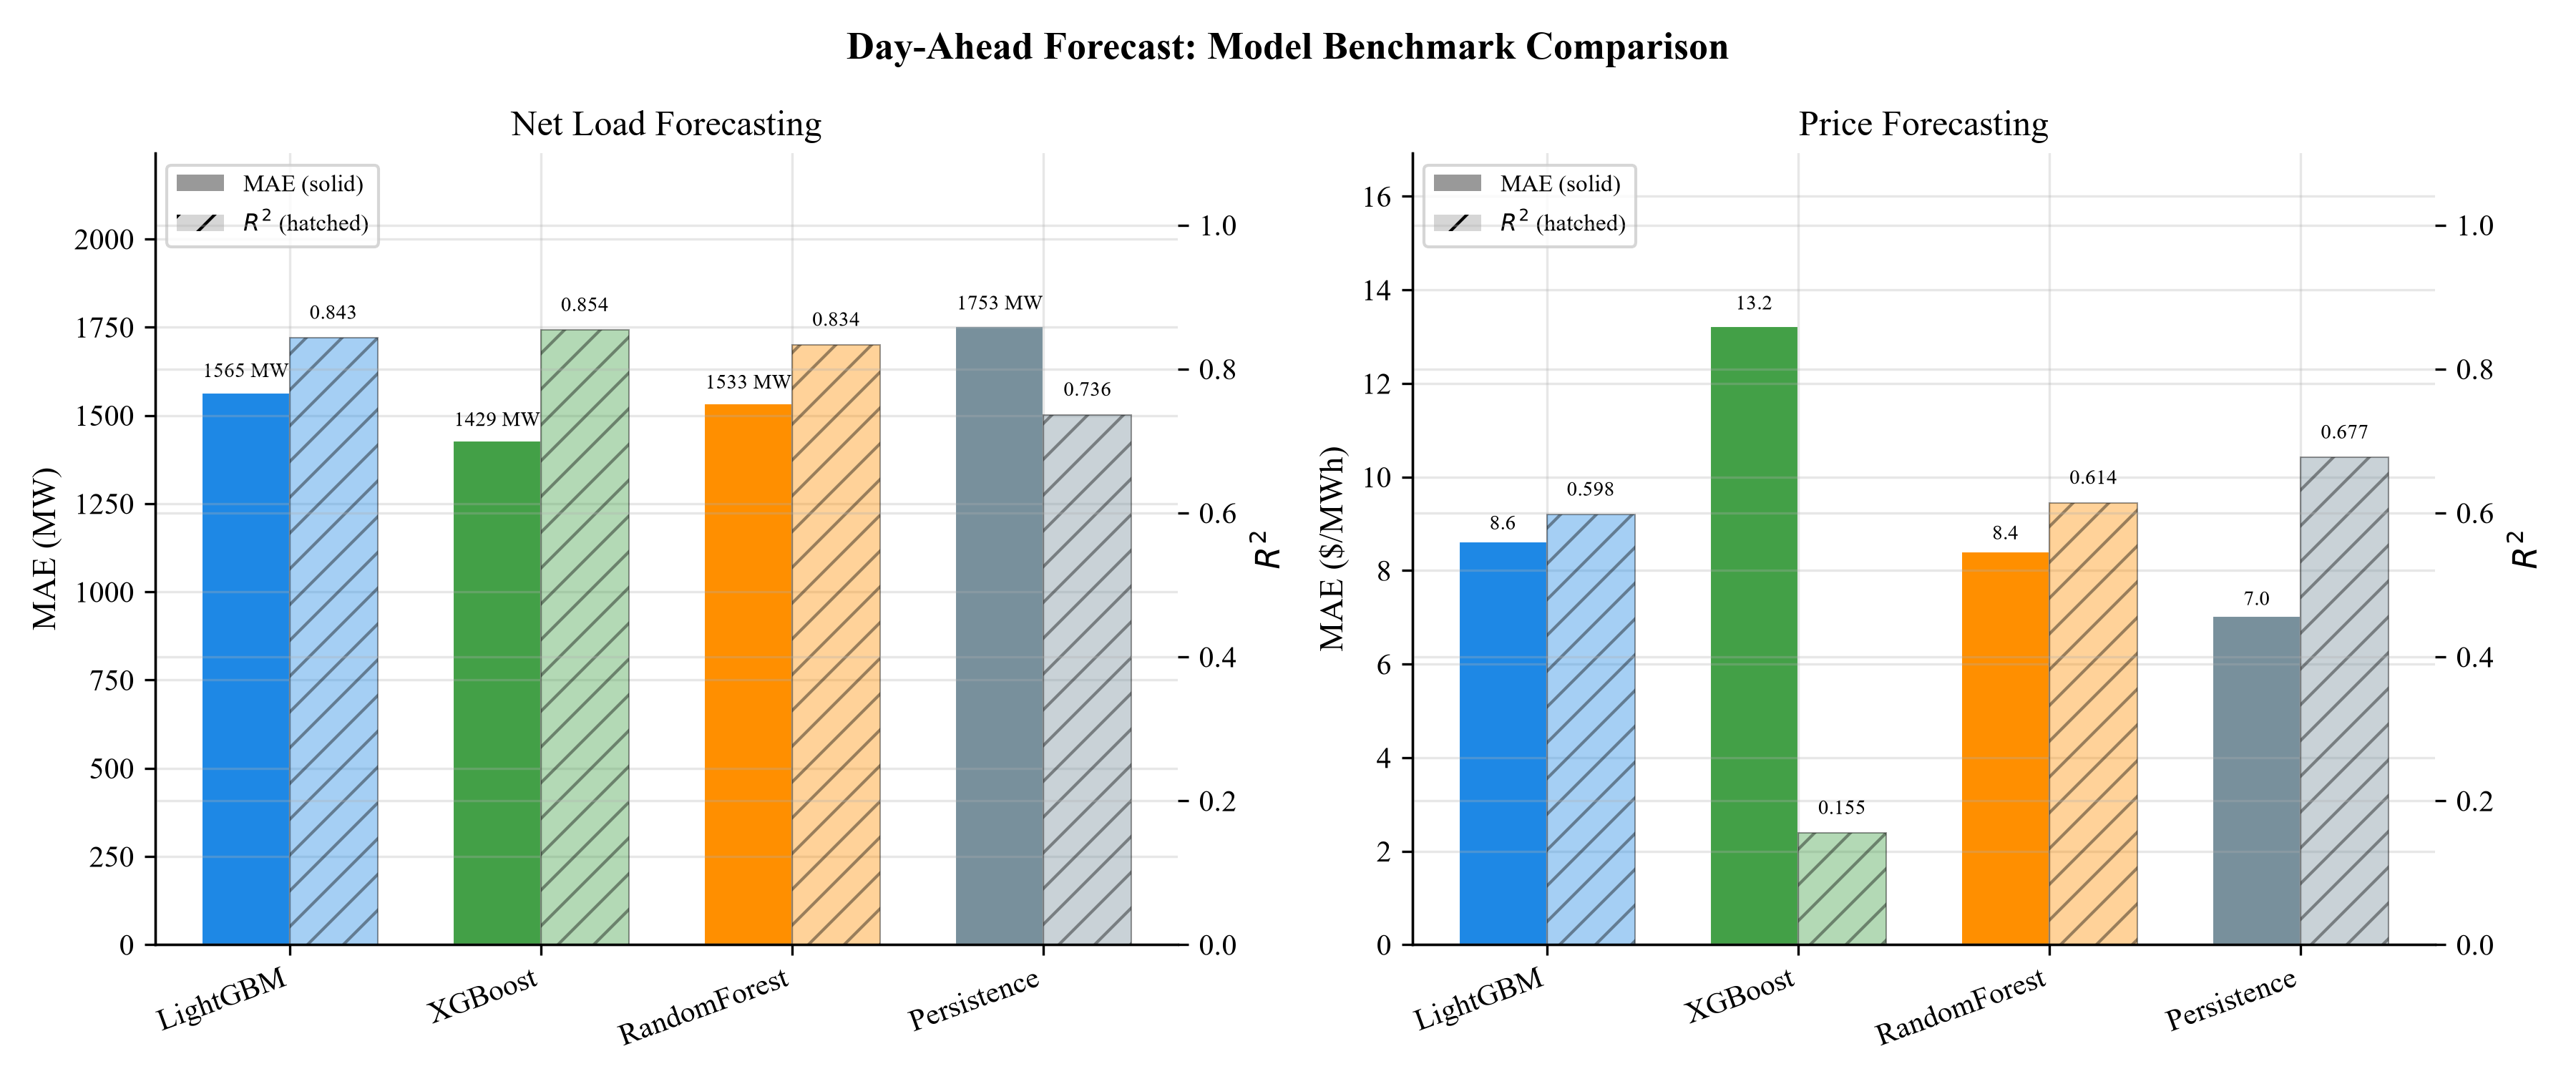
\includegraphics[width=\textwidth]{fig06_benchmark_comparison.png}
\caption{Forecasting benchmark: MAE (solid bars) and $R^2$ (hatched bars) across models, including the persistence baseline.}
\label{fig:bench}
\end{figure}

\textbf{Cross-validation detail.} Table~\ref{tab:cv} reports the full five-fold expanding-window breakdown underlying Section~\ref{sec:results_cv}. Fold~2 (July~10 -- August~21, $R^2 = 0.719$) coincides with the 2023 California heat events, when air-conditioning-driven demand spikes deviate from the historical patterns embedded in lag features. Forecast error correlates weakly but positively with temperature ($r = 0.162$, Fig.~\ref{fig:errtemp}), with the largest errors on days exceeding 35$^\circ$C in the Central Valley, motivating the weather-ensemble extension identified as future work (Section~\ref{sec:conclusion}).

\begin{table}[htbp]
\centering
\caption{Expanding-window cross-validation (LightGBM, net load).}
\label{tab:cv}
\small
\resizebox{\textwidth}{!}{%
\begin{tabular}{cccrrr}
\toprule
\textbf{Fold} & \textbf{Train end} & \textbf{Test end} & \textbf{MAE (MW)} & \textbf{RMSE (MW)} & \textbf{$R^2$} \\
\midrule
1 & May 29 & Jul 10 & 1{,}203 & 1{,}855 & 0.926 \\
2 & Jul 10 & Aug 21 & 2{,}711 & 3{,}737 & 0.719 \\
3 & Aug 21 & Oct 3  & 1{,}451 & 2{,}044 & 0.922 \\
4 & Oct 3  & Nov 15 & 1{,}335 & 1{,}821 & 0.925 \\
5 & Nov 15 & Dec 31 & 1{,}457 & 2{,}008 & 0.850 \\
\midrule
\multicolumn{3}{c}{Mean $\pm$ std} & $1{,}632 \pm 612$ & $2{,}293 \pm 813$ & $0.869 \pm 0.089$ \\
\bottomrule
\end{tabular}}
\end{table}

\begin{figure}[htbp]
\centering
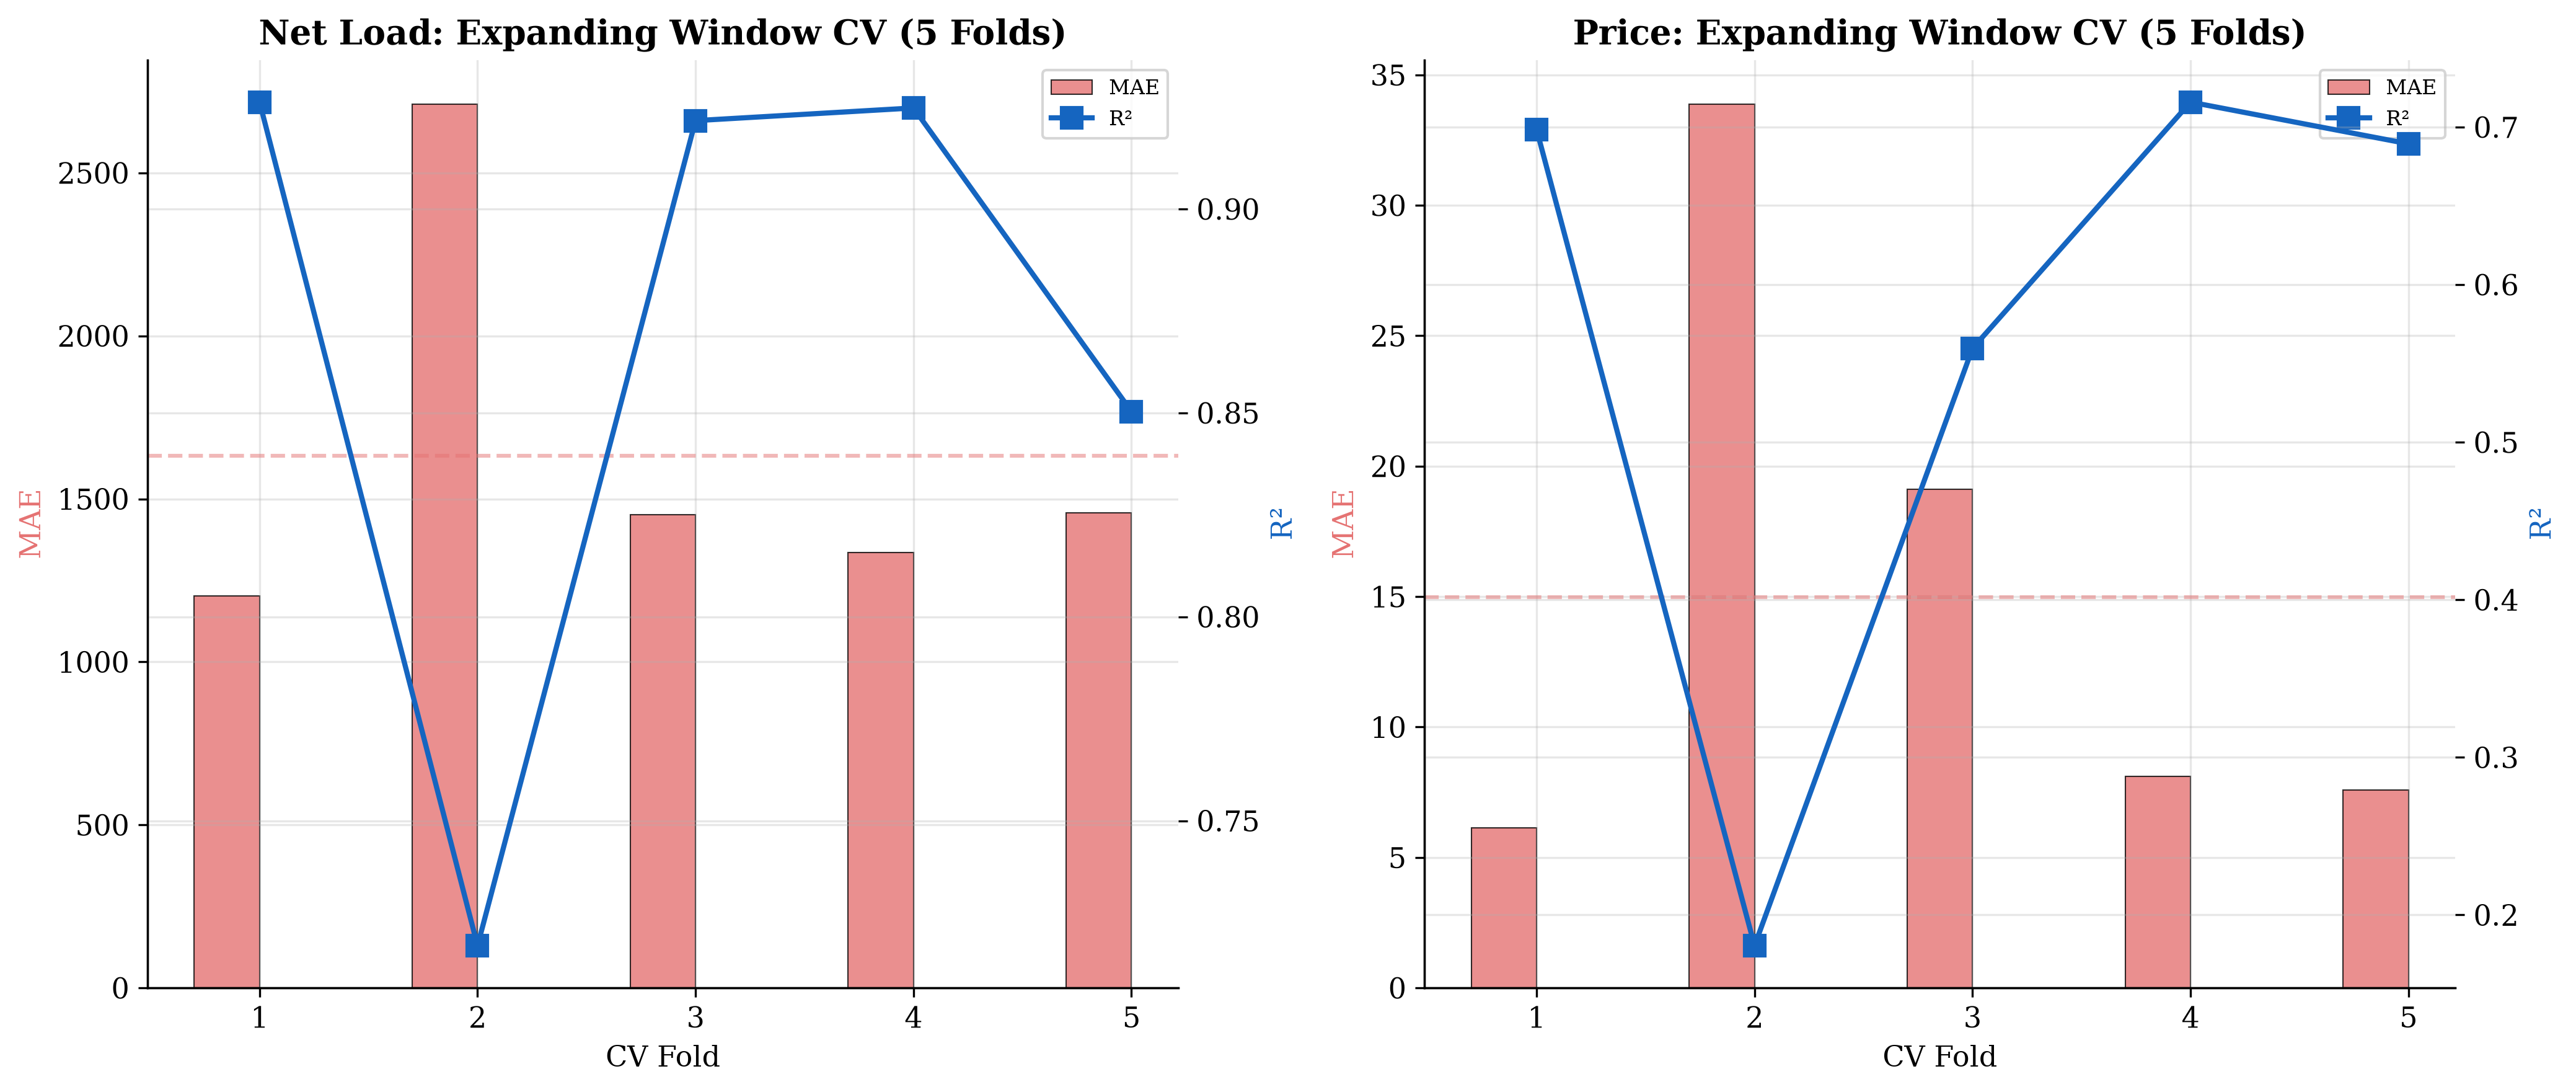
\includegraphics[width=\textwidth]{fig16_cv_stability.png}
\caption{Expanding-window cross-validation stability: MAE (bars) and $R^2$ (line) across five folds.}
\label{fig:cvfig}
\end{figure}

\begin{figure}[htbp]
\centering
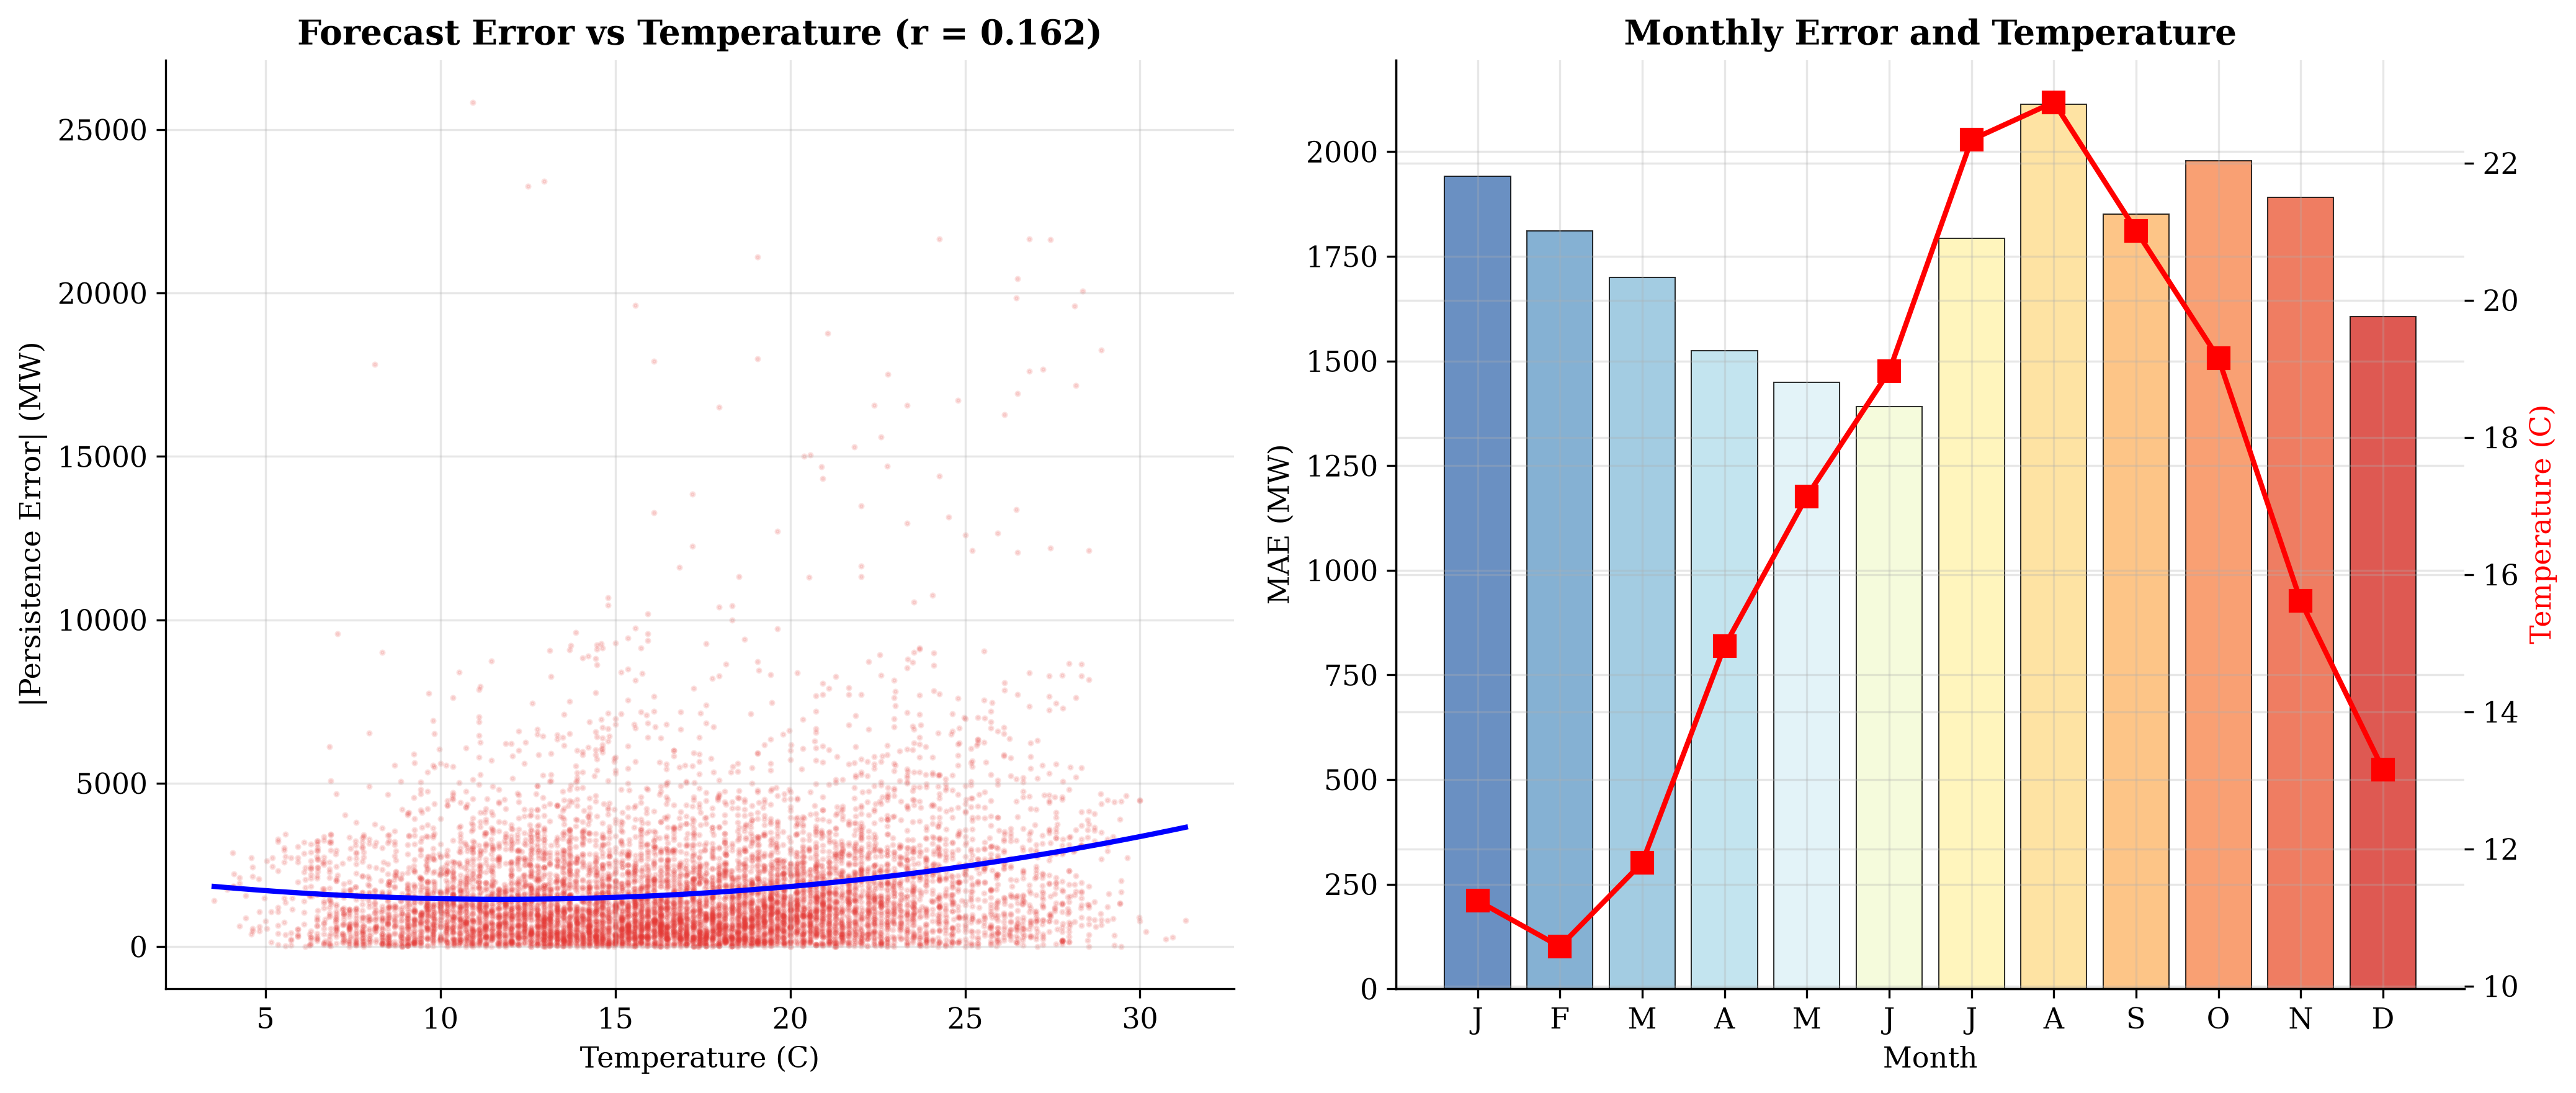
\includegraphics[width=\textwidth]{fig_error_vs_temperature.png}
\caption{Forecast error vs.\ temperature ($r = 0.162$): largest errors concentrate on extreme heat days.}
\label{fig:errtemp}
\end{figure}

\begin{figure}[htbp]
\centering
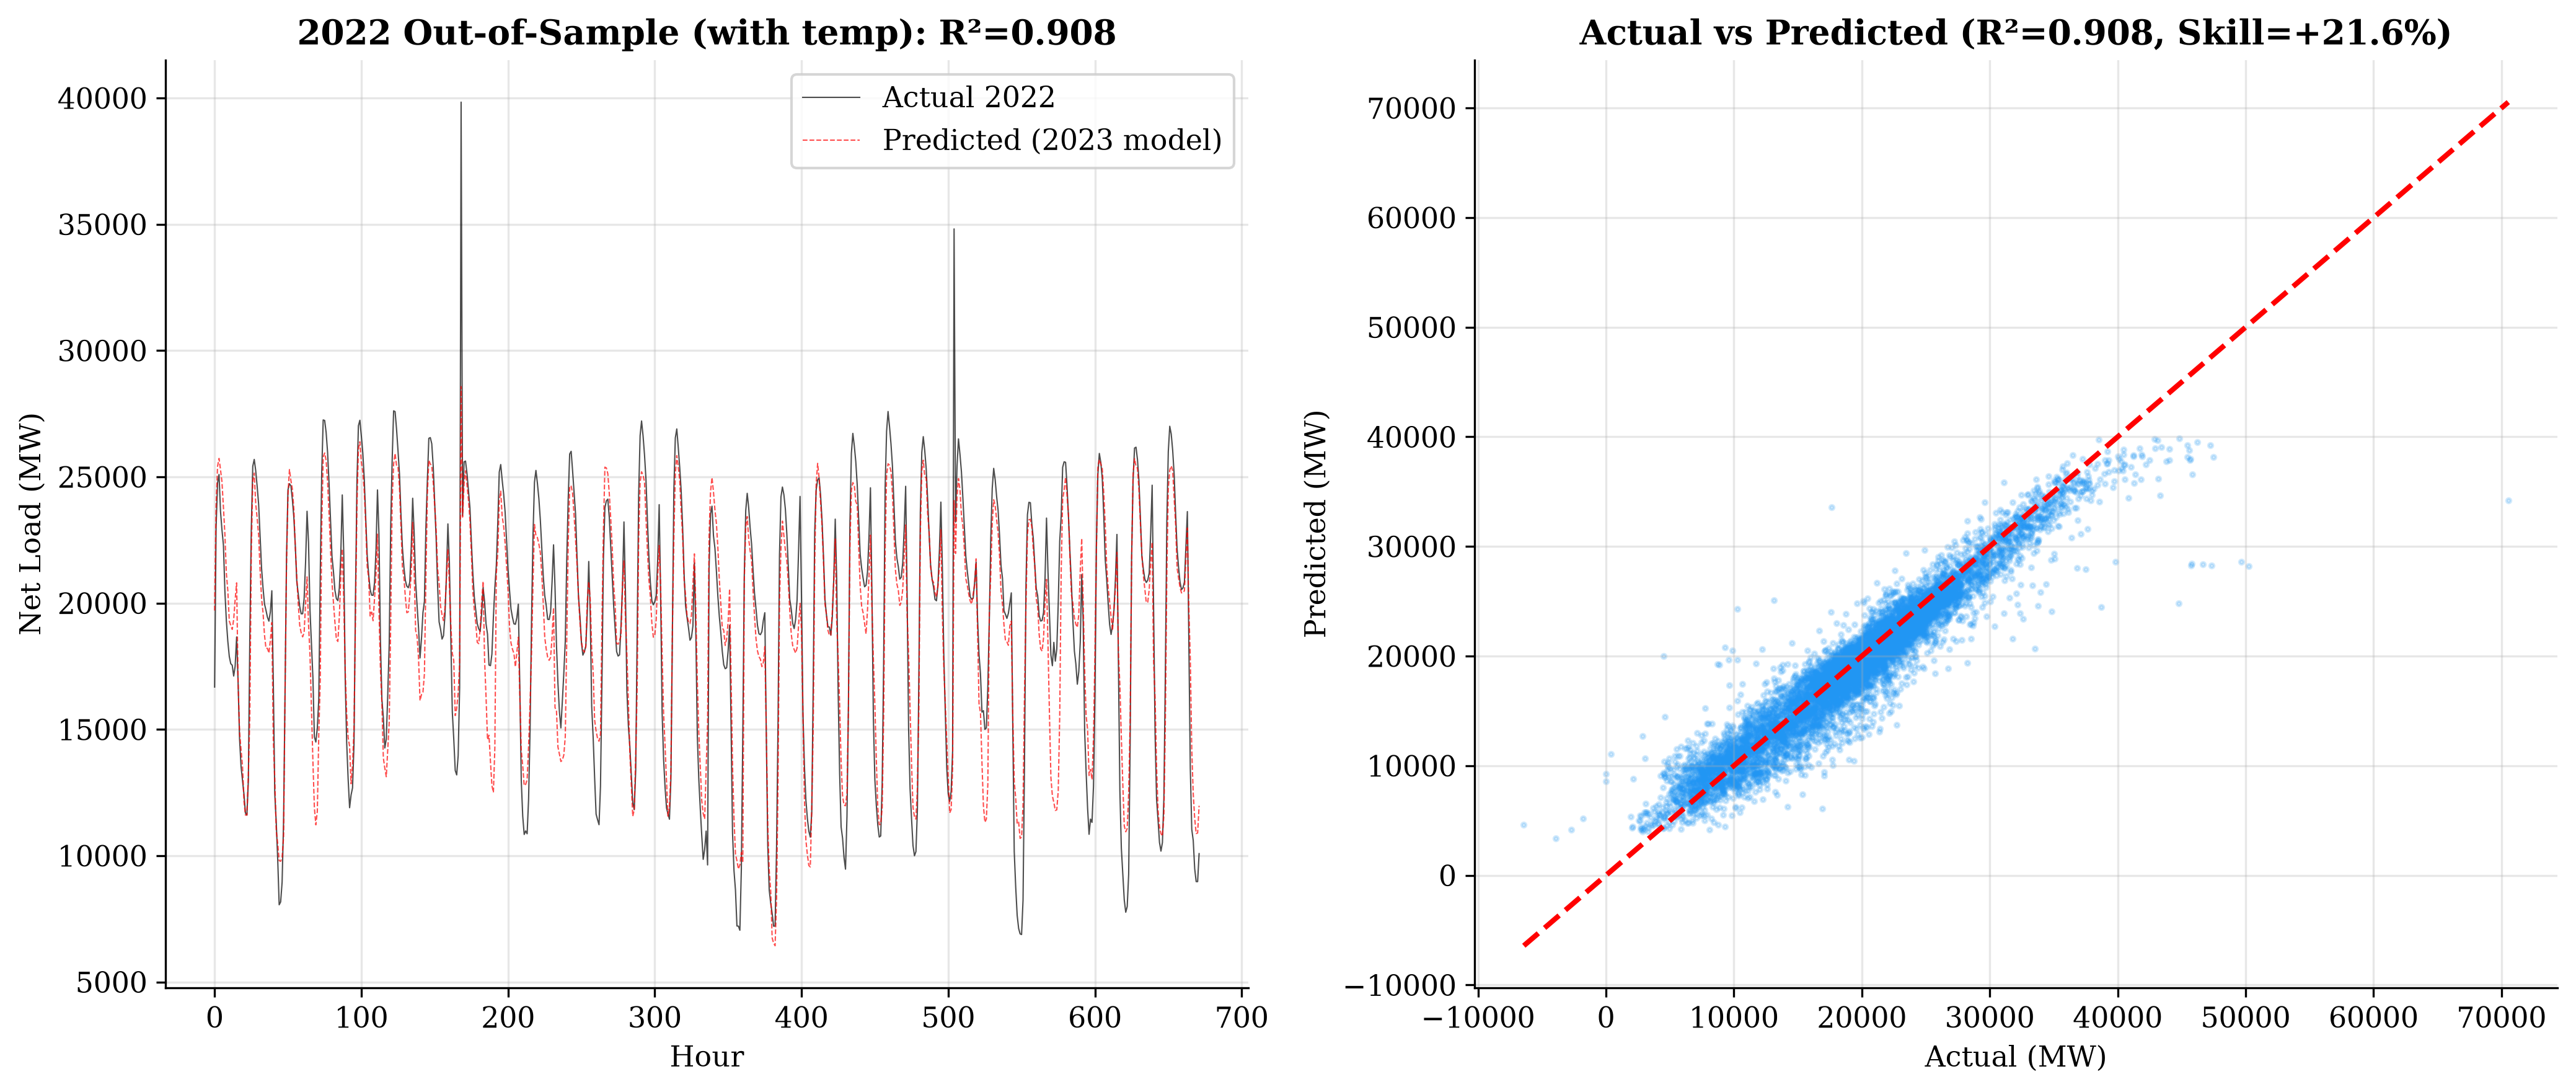
\includegraphics[width=\textwidth]{fig_2022_validation.png}
\caption{Out-of-sample generalization: 2023-trained model applied to 2022 ($R^2 = 0.908$, MAE = 1{,}514~MW, $n = 8{,}593$).}
\label{fig:oos}
\end{figure}

\begin{figure}[htbp]
\centering
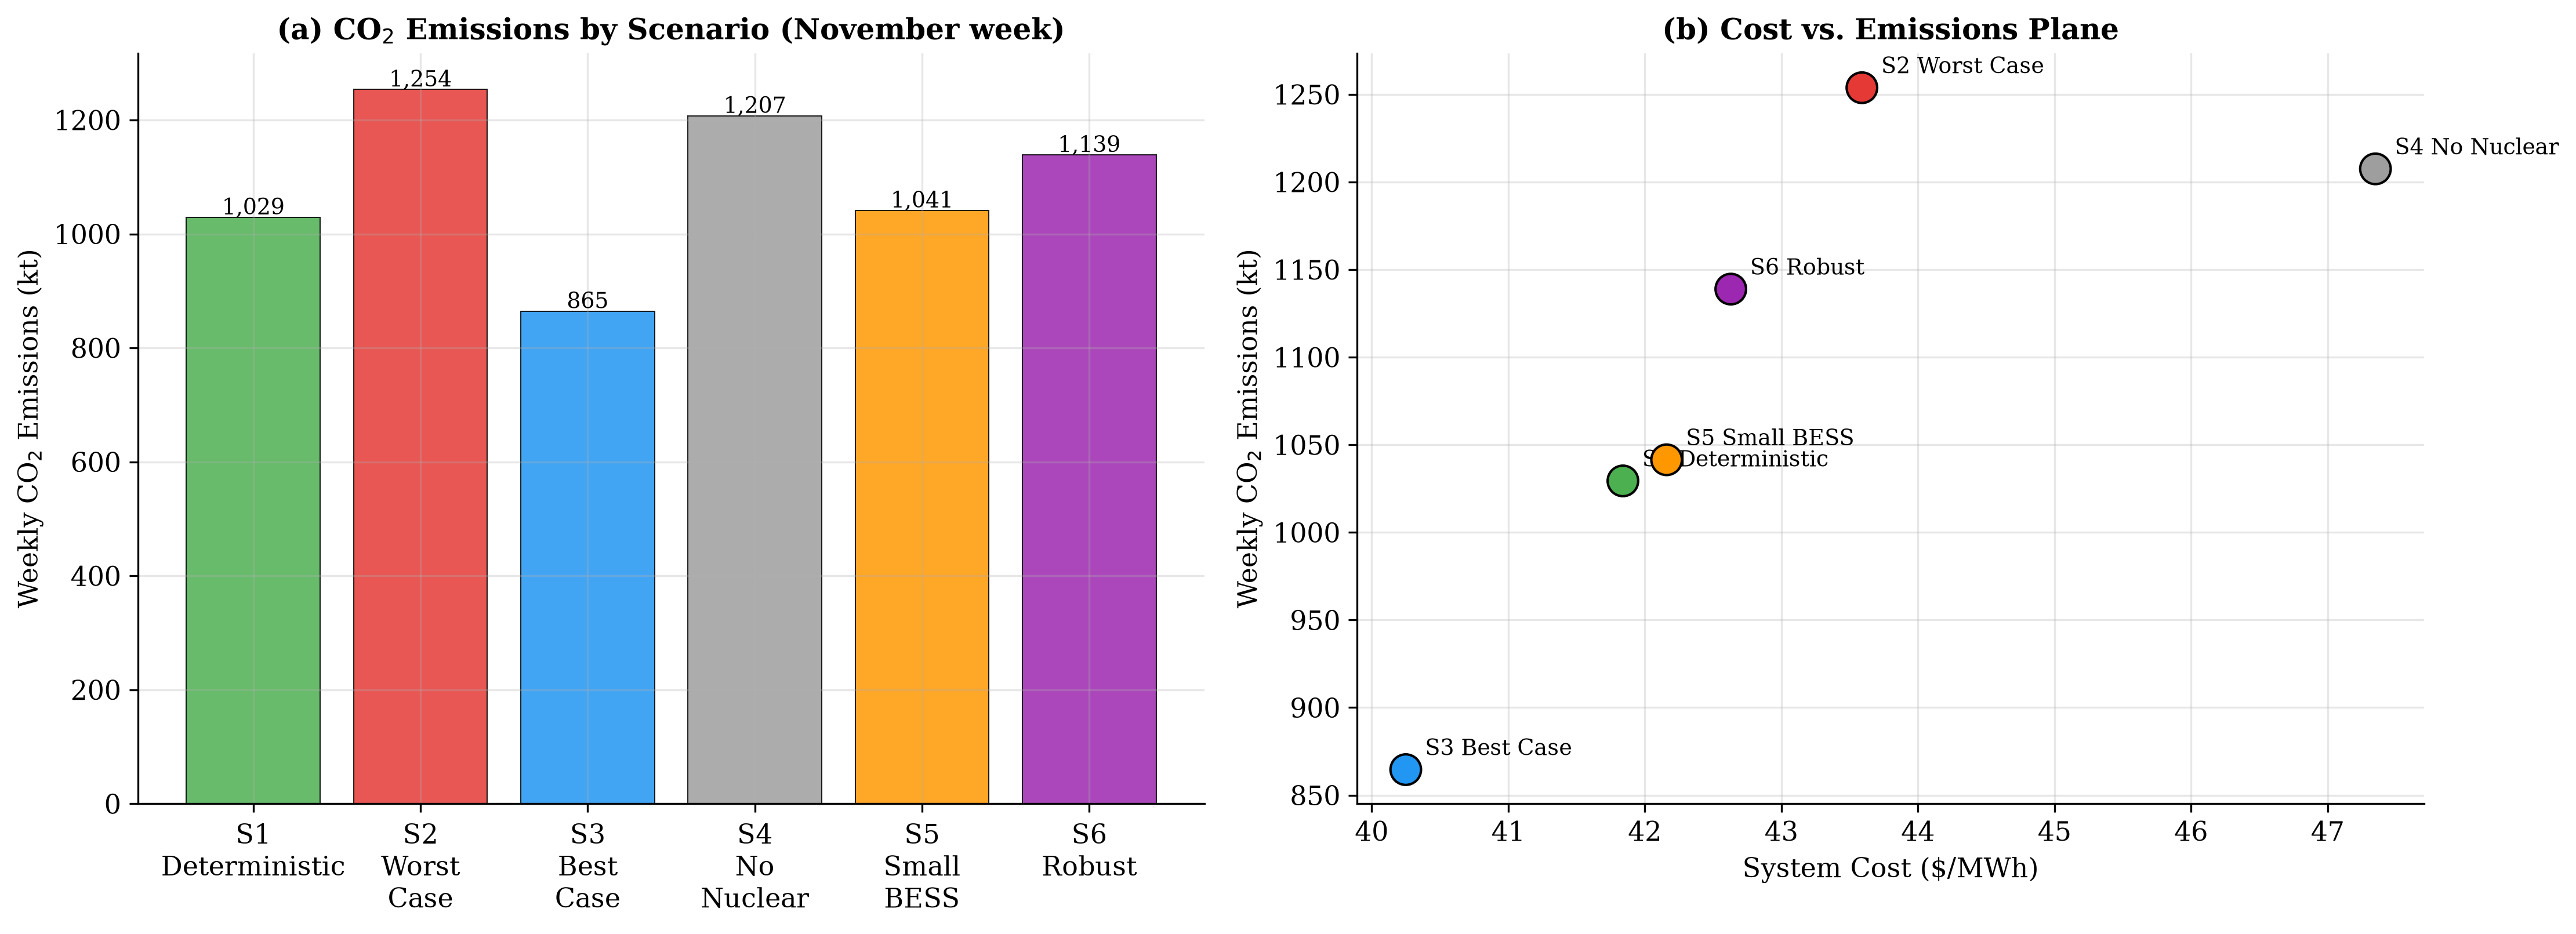
\includegraphics[width=\textwidth]{fig_co2_analysis.png}
\caption{CO$_2$ emissions by scenario (November week, two-tier UC model; factors: CCGT 0.37, peaker 0.55, imports 0.428~t/MWh, the CARB unspecified-import default). S1 = 1{,}029~kt; S4 (no nuclear) = 1{,}207~kt ($+17.3\%$), ${\sim}9.3$~Mt/year annualized.}
\label{fig:co2}
\end{figure}

\begin{figure}[htbp]
\centering
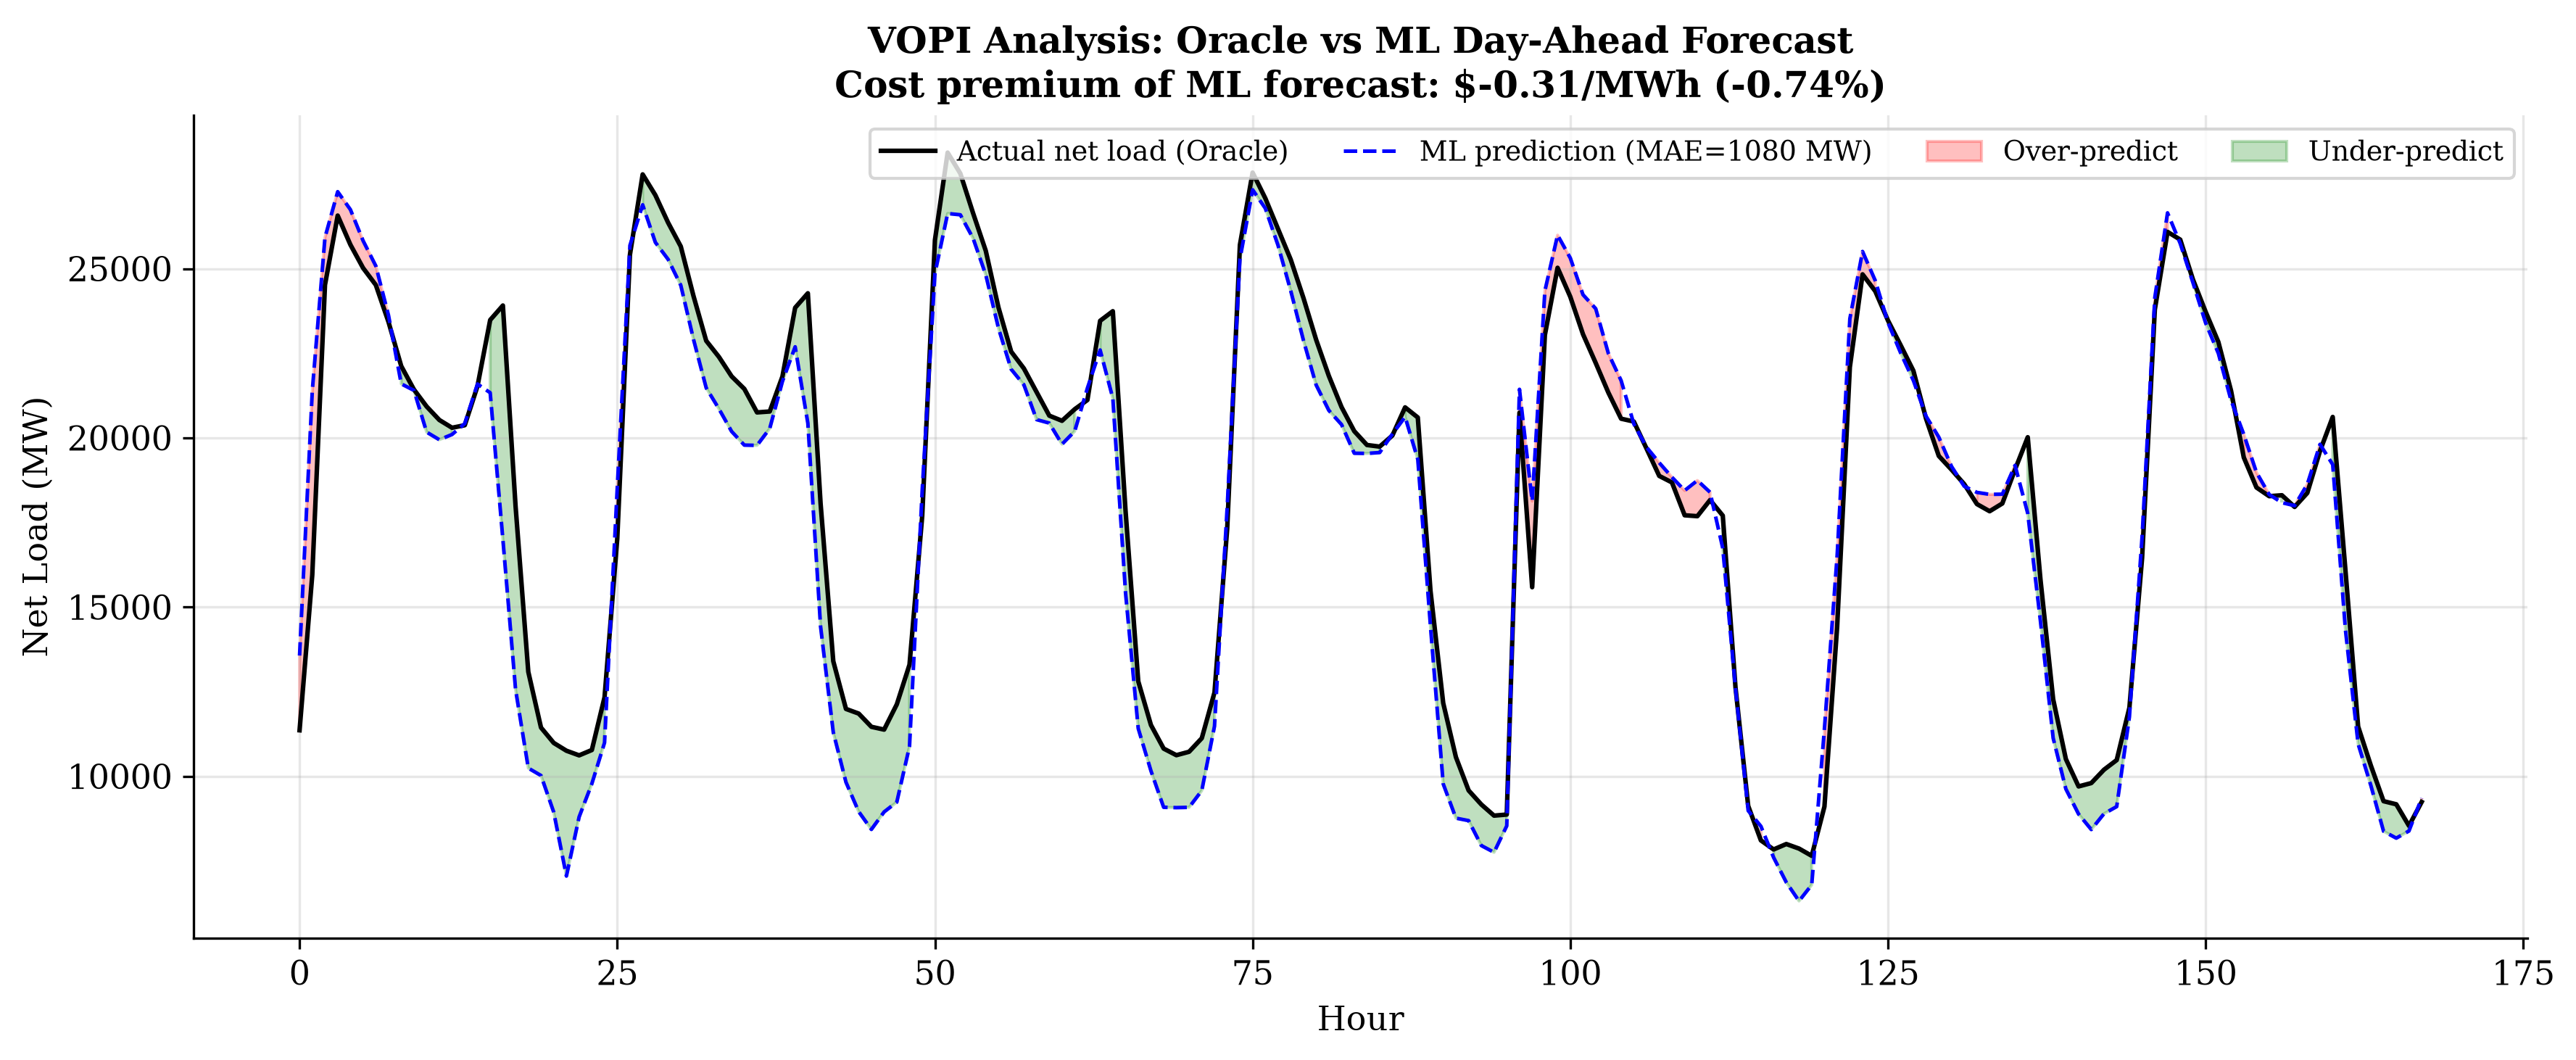
\includegraphics[width=\textwidth]{fig_vopi_analysis.png}
\caption{Value of perfect information: oracle (\$42.15/MWh) vs.\ ML-based dispatch (\$41.84/MWh); $|\Delta| = \$0.31$/MWh (0.74\%).}
\label{fig:vopi}
\end{figure}

\begin{figure}[htbp]
\centering
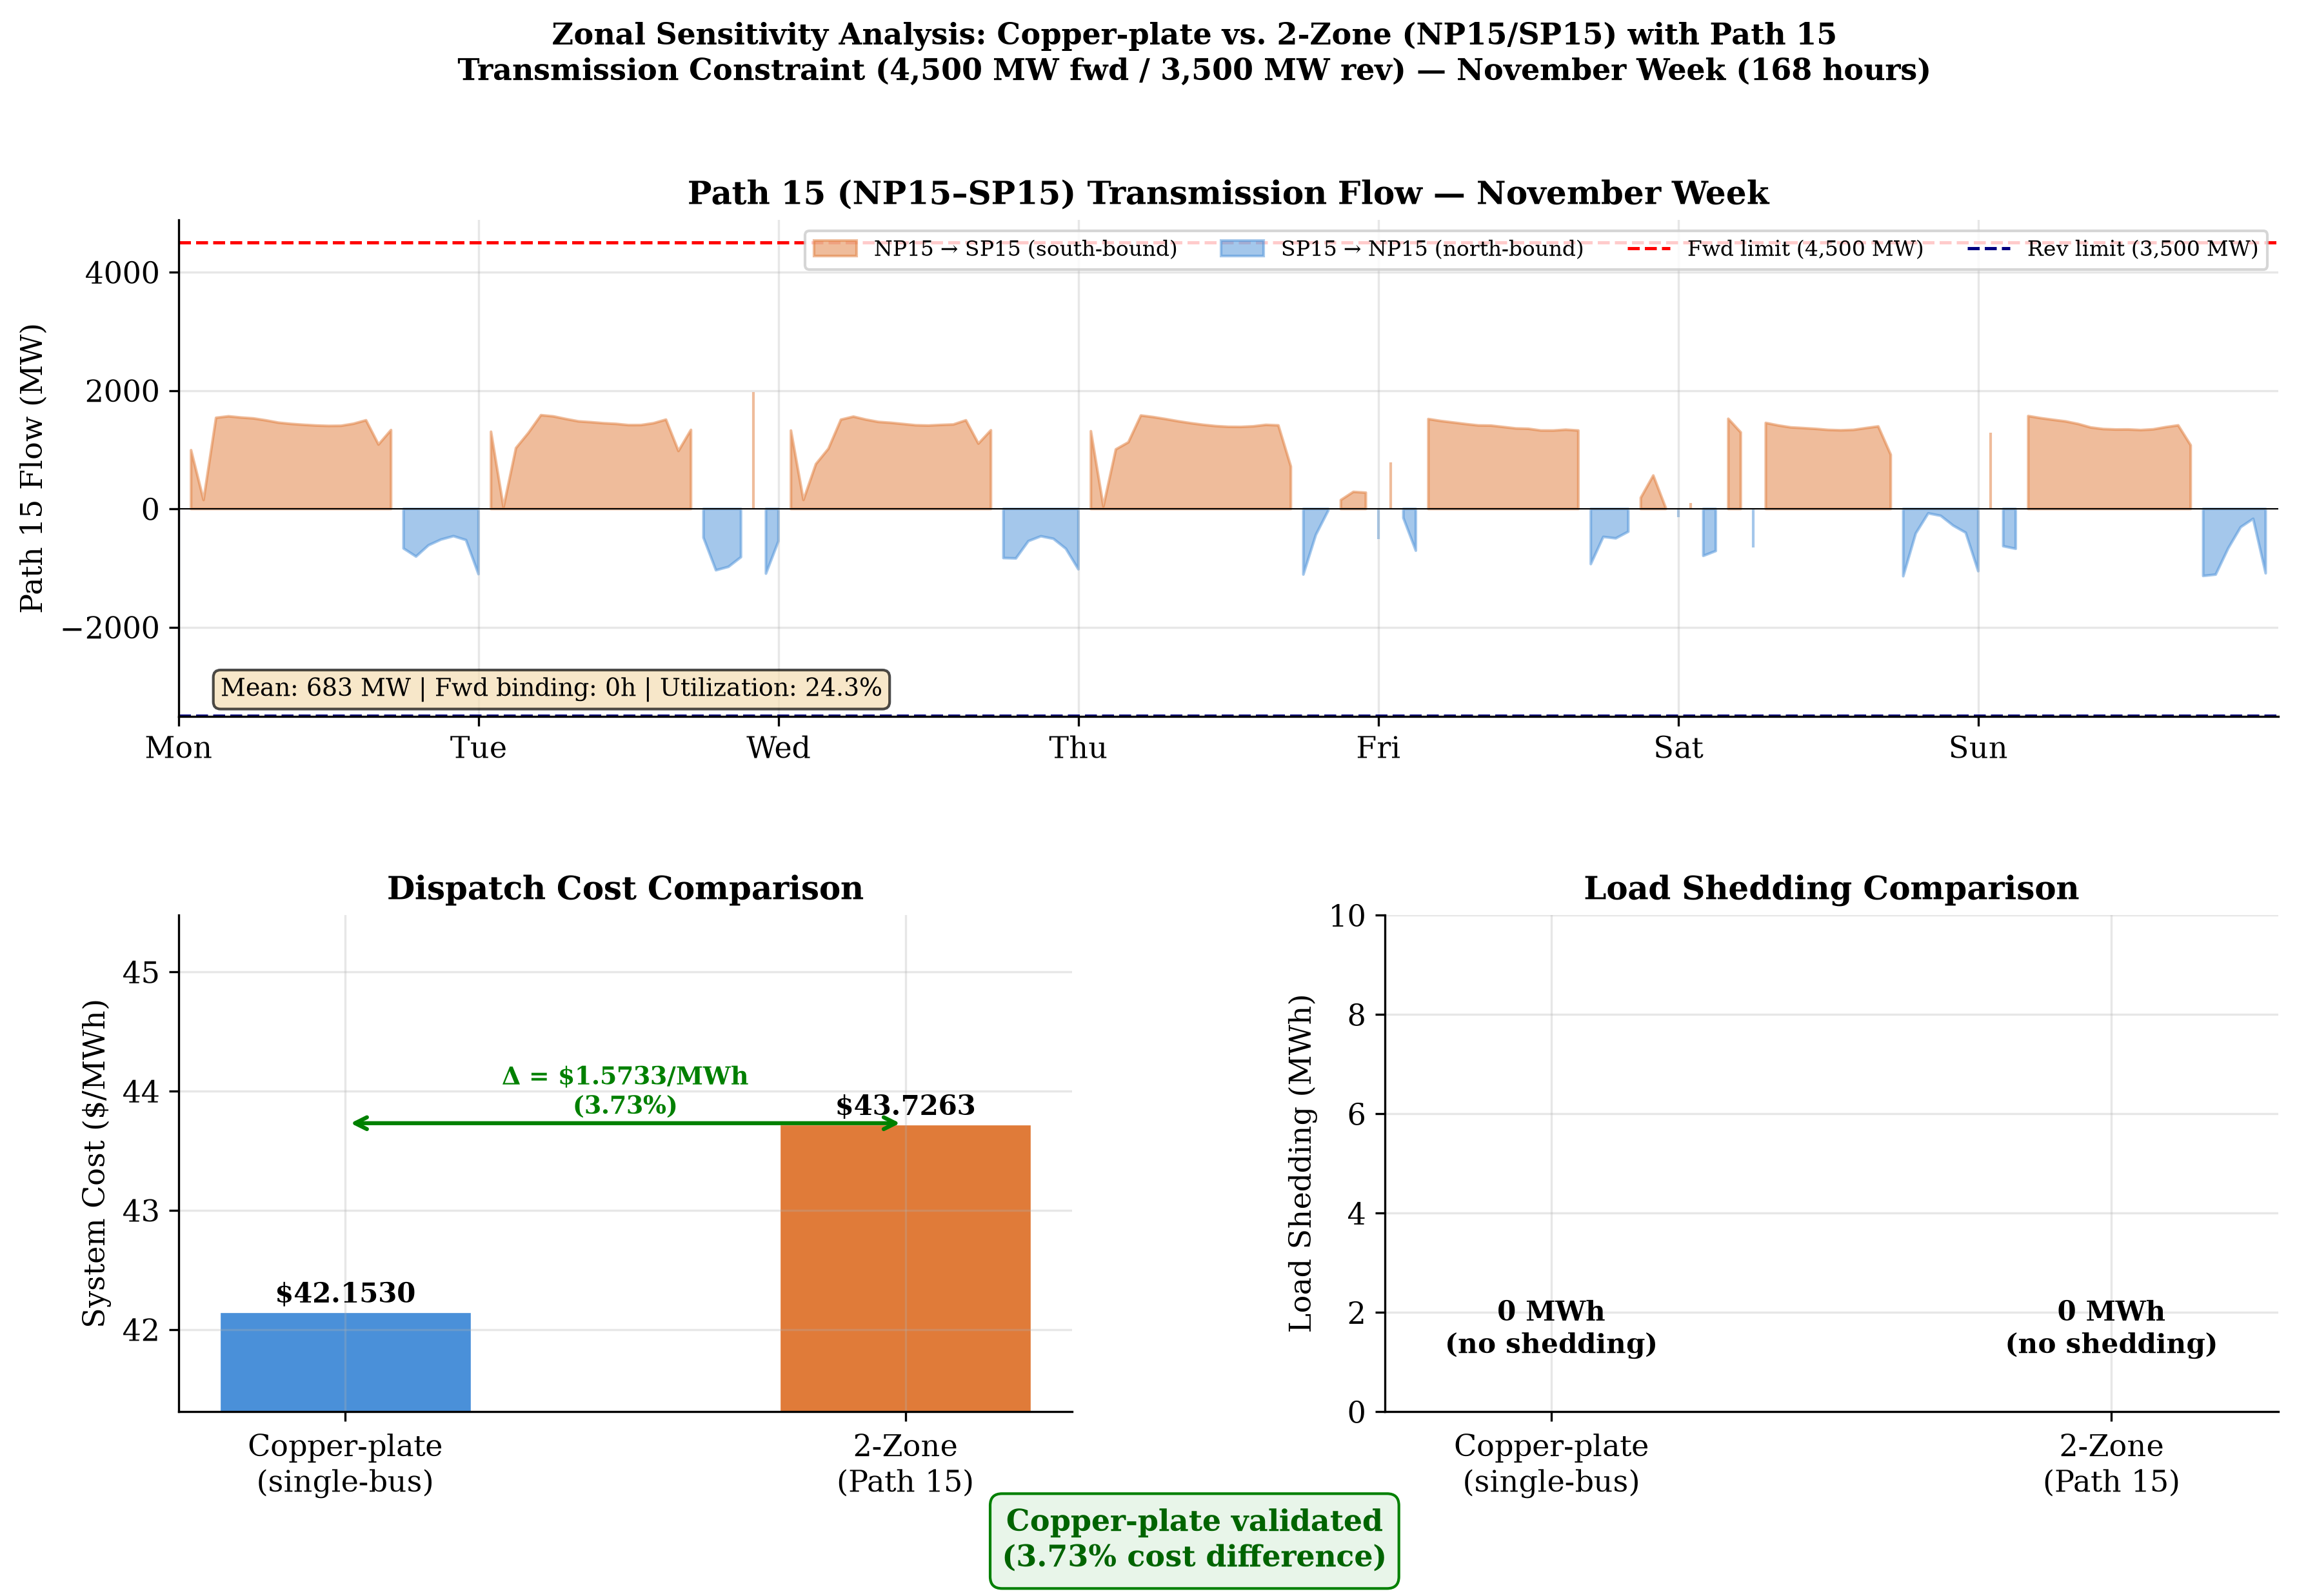
\includegraphics[width=\textwidth]{fig_zonal_sensitivity.png}
\caption{Copper-plate vs.\ two-zone (NP15/SP15, Path~15 limit 4{,}500/3{,}500~MW): $+3.7\%$ cost difference; Path~15 binds in 0 of 168 hours.}
\label{fig:zonal}
\end{figure}

\begin{figure}[htbp]
\centering
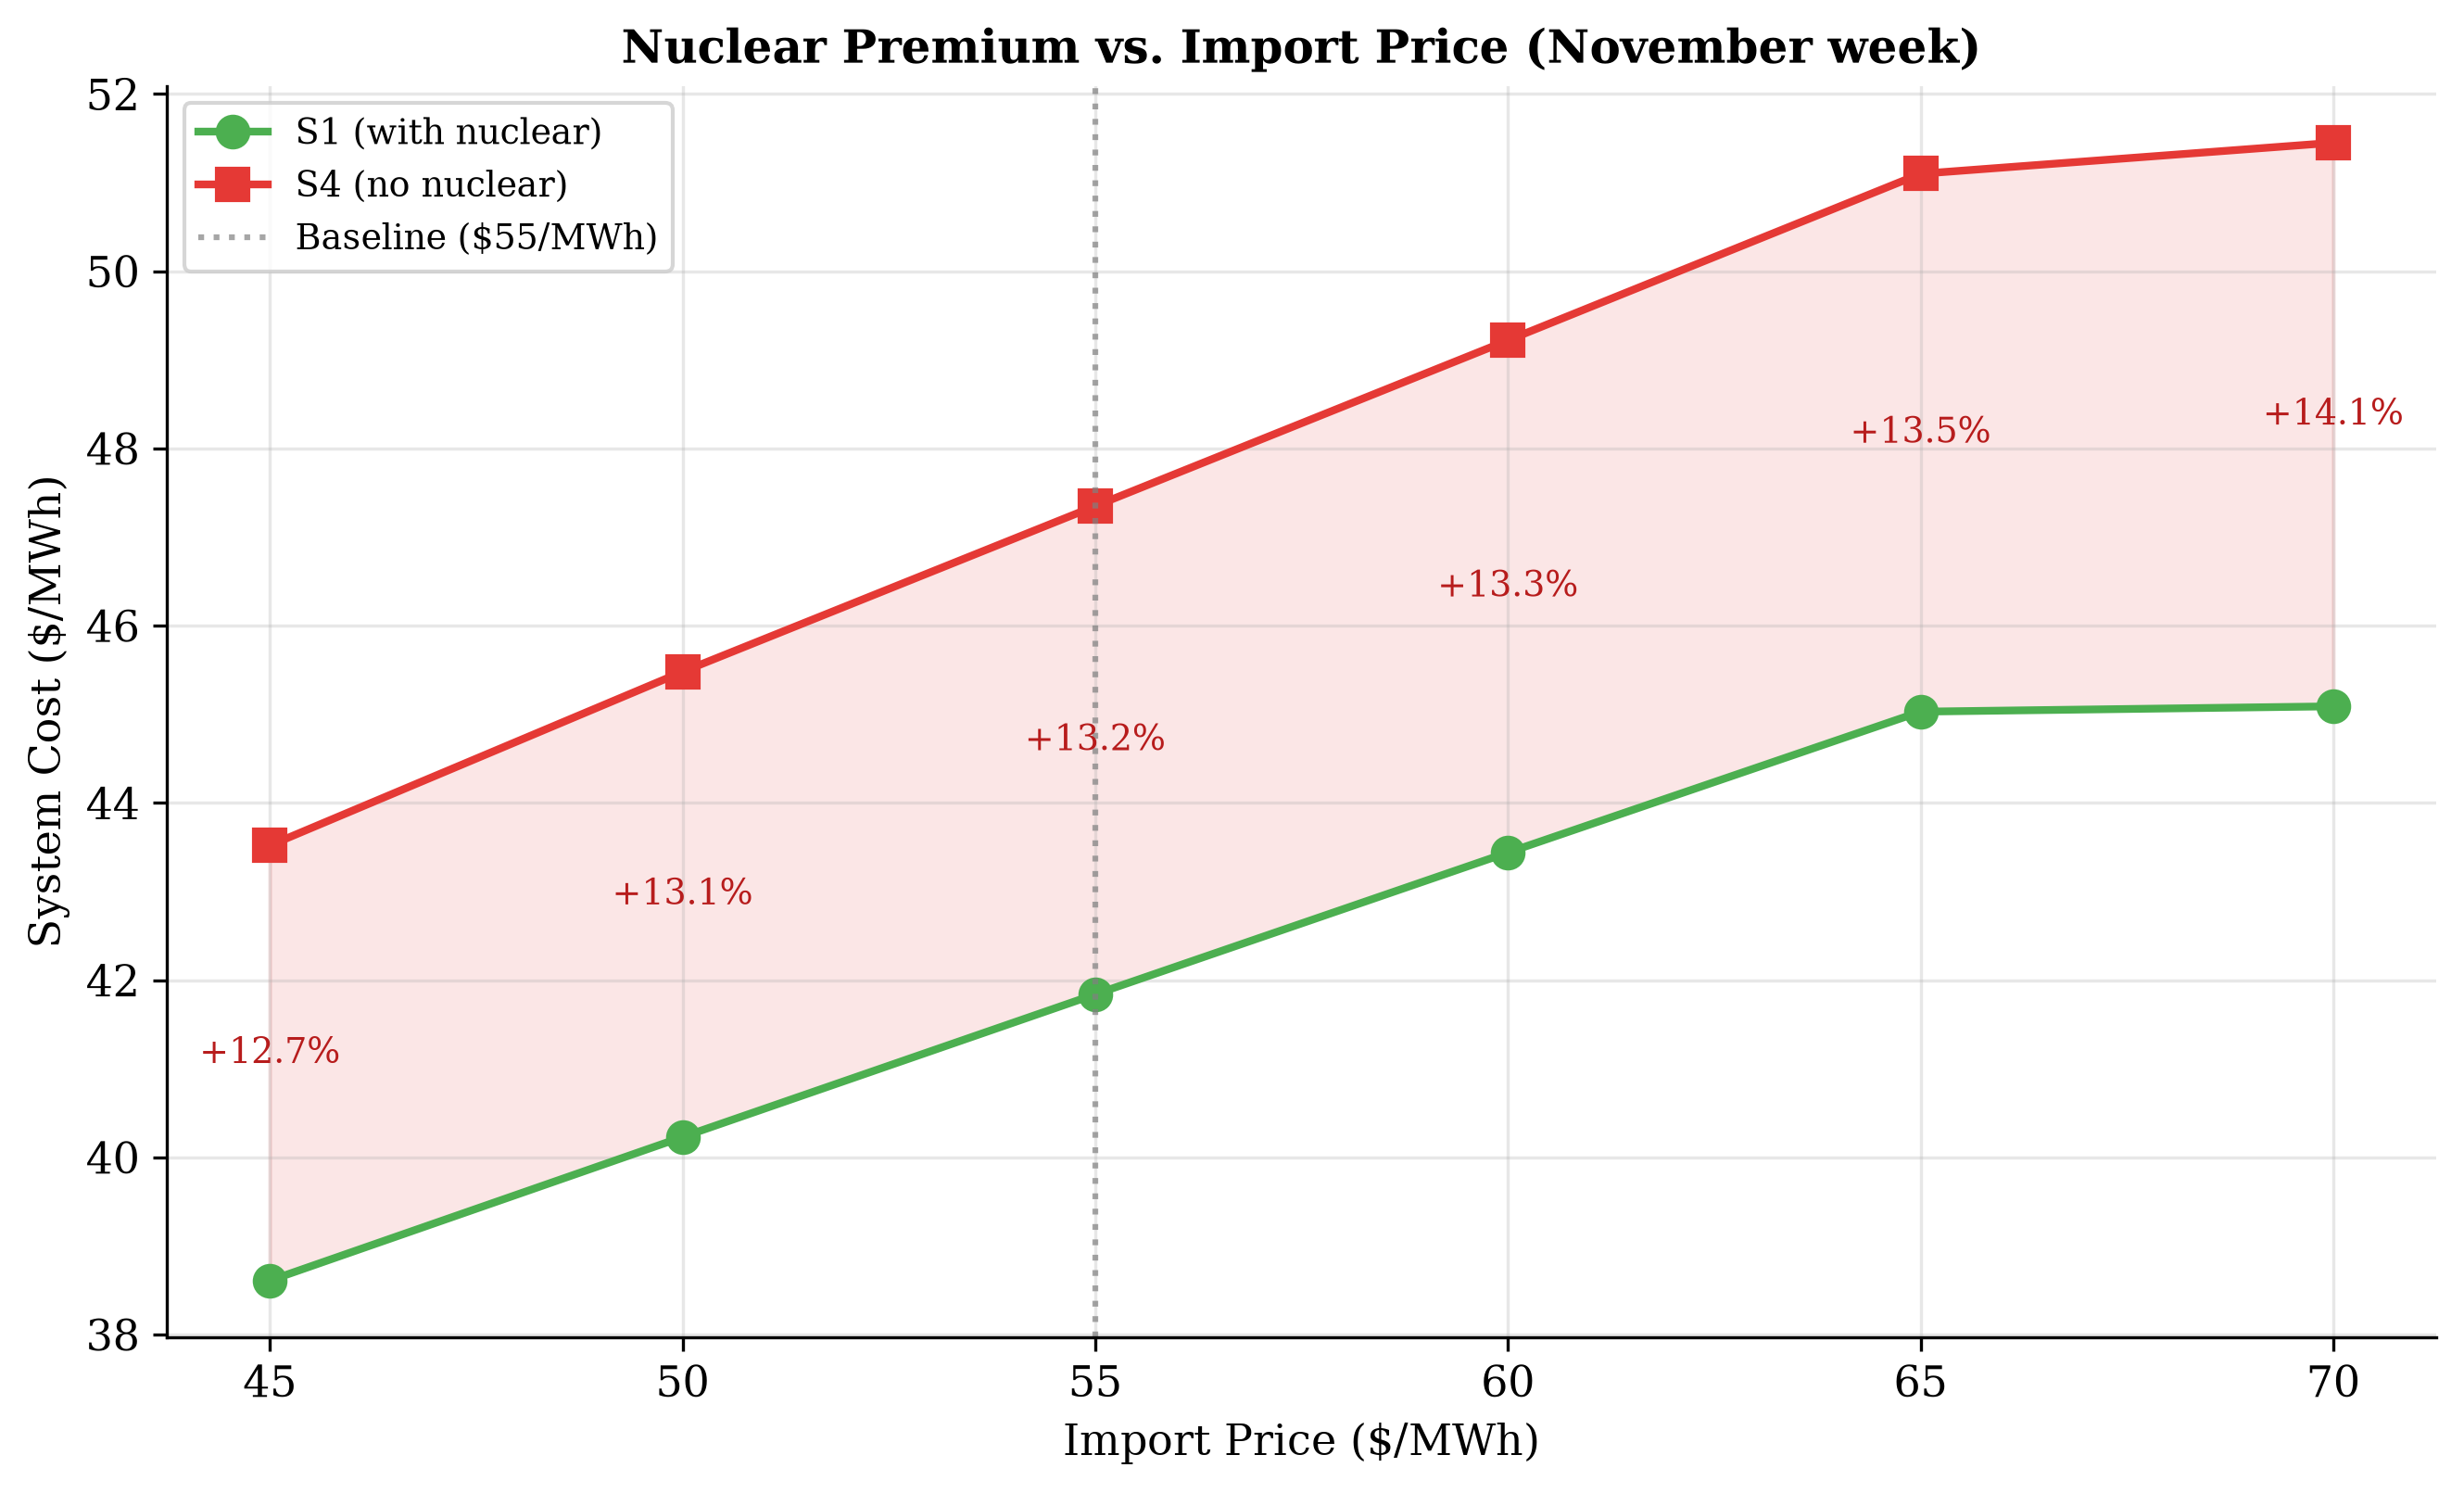
\includegraphics[width=0.8\textwidth]{fig_import_sensitivity.png}
\caption{Nuclear premium vs.\ import price (\$45--\$70/MWh): the S4$-$S1 premium (annotated) remains within $+12.7$ to $+14.1\%$; both curves flatten above \$65/MWh as imports exit the merit order.}
\label{fig:impsens}
\end{figure}

\begin{figure}[htbp]
\centering
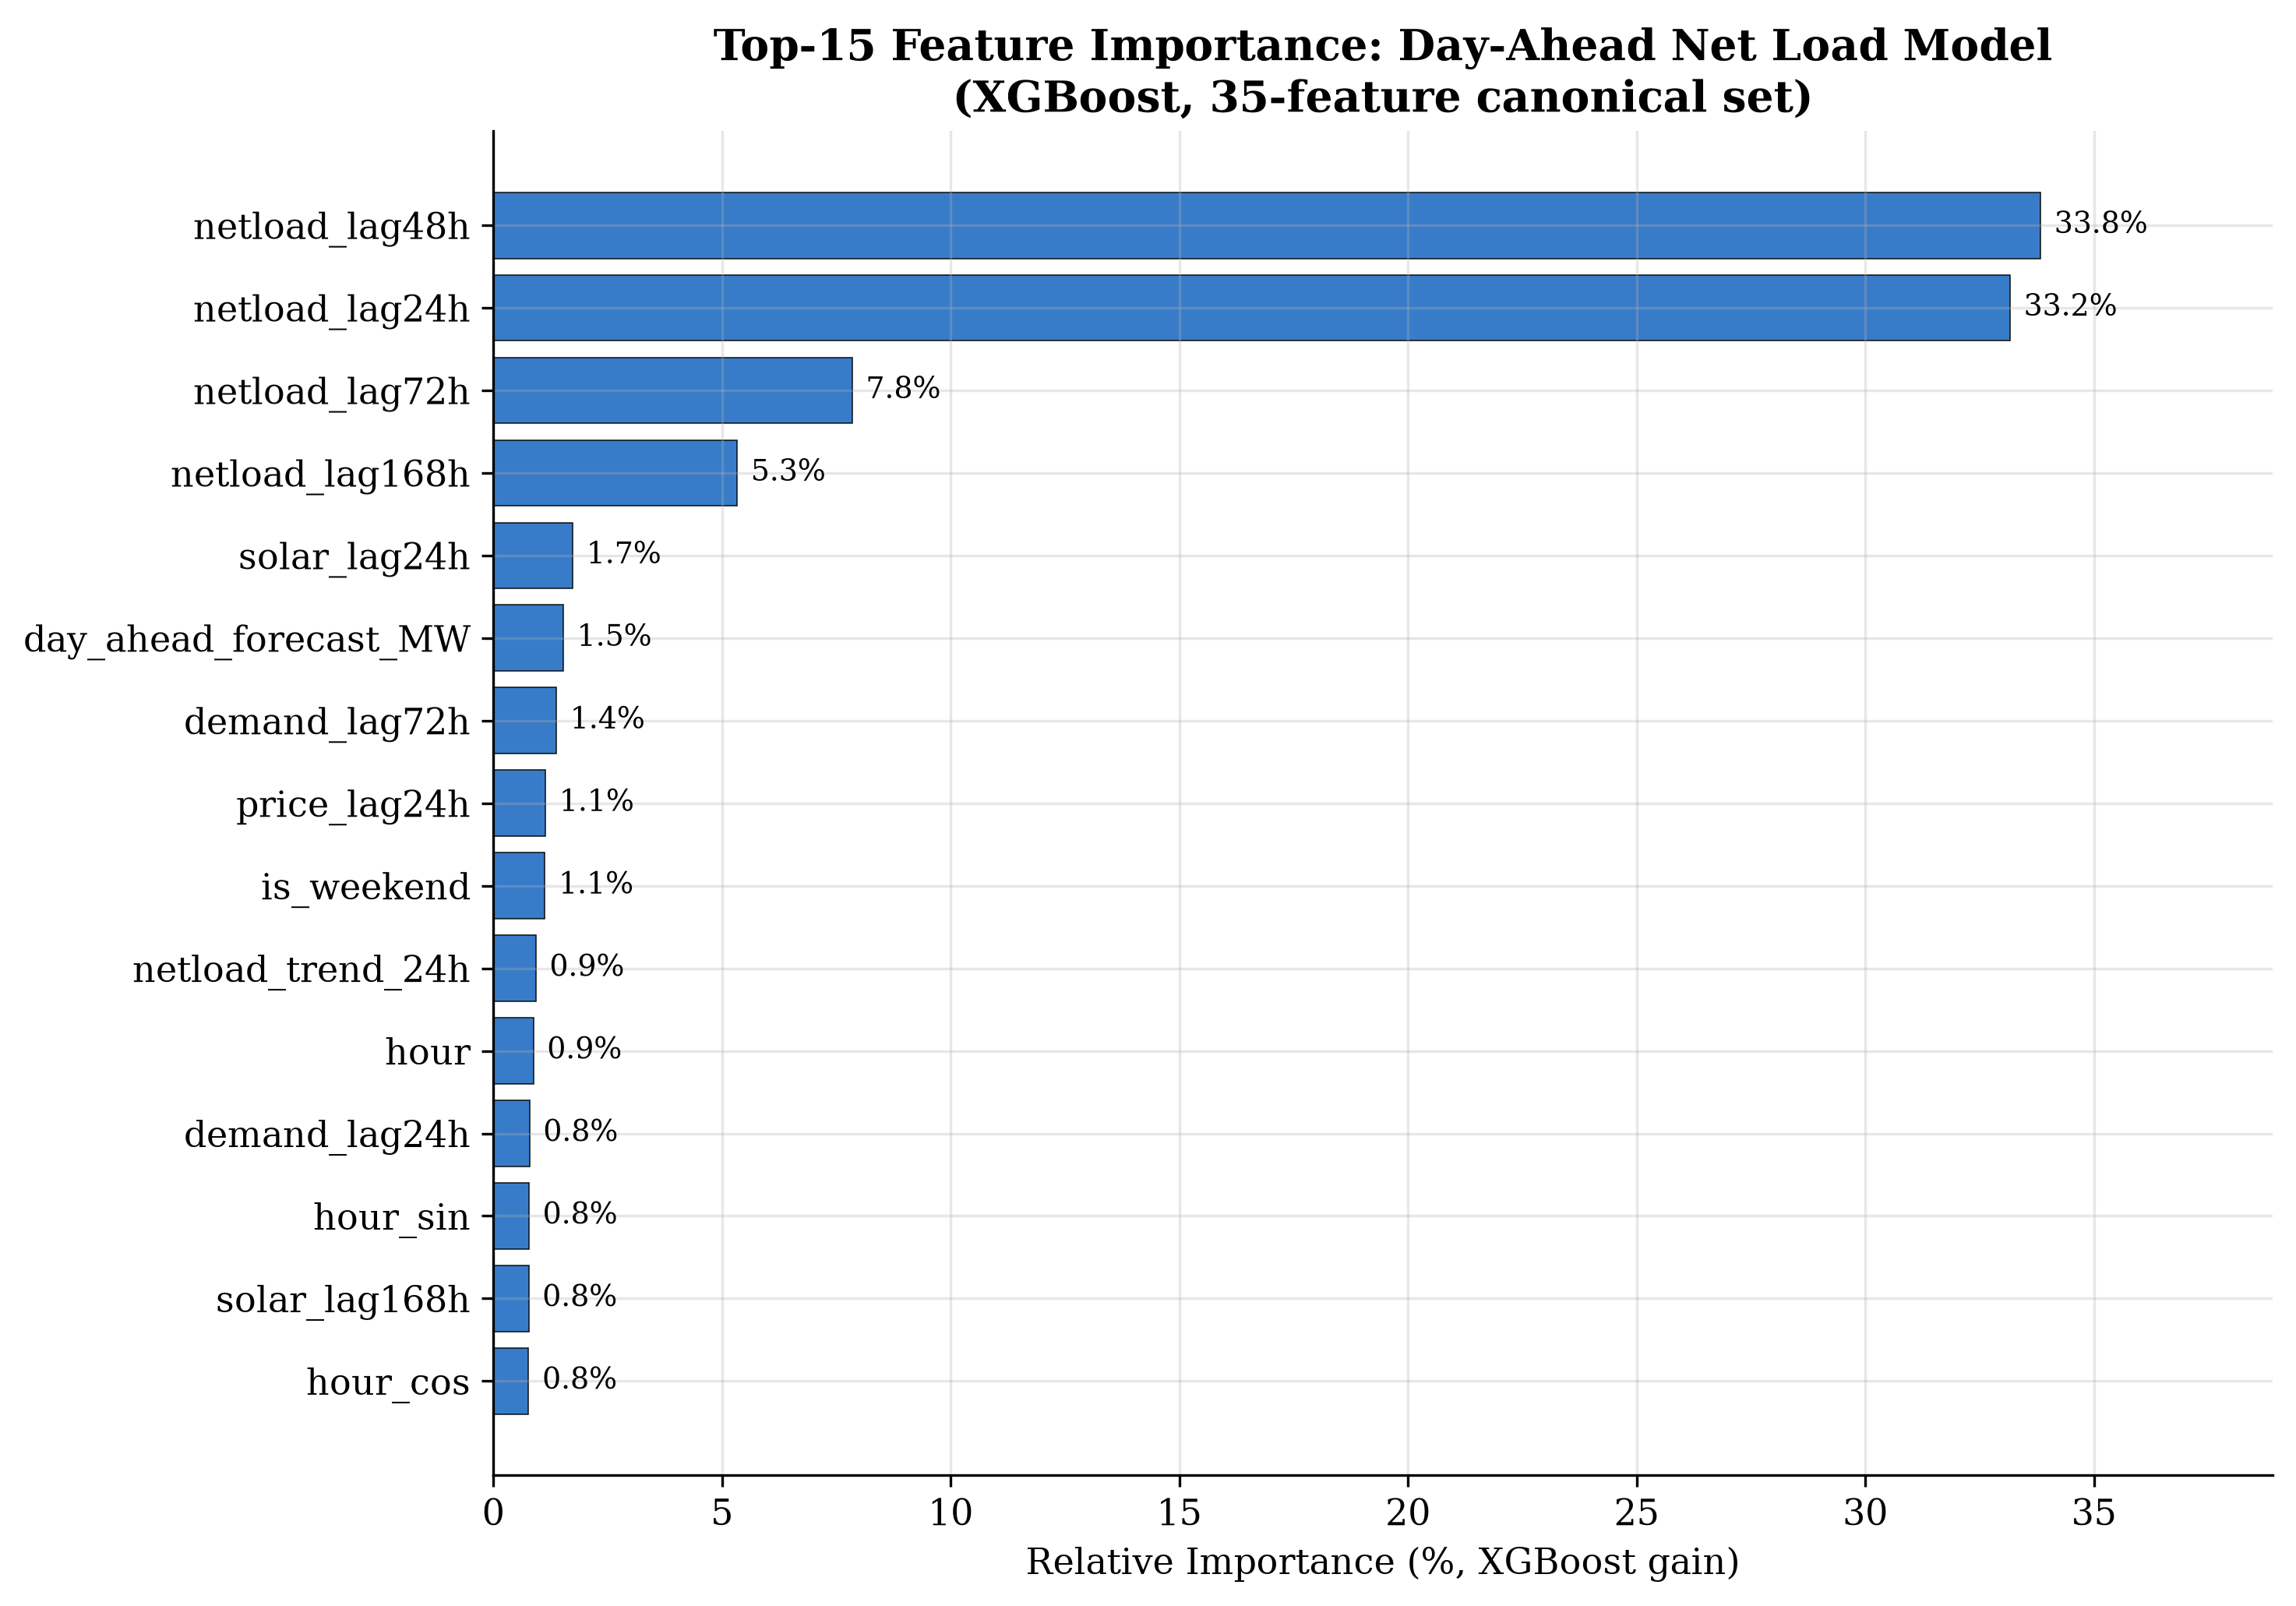
\includegraphics[width=0.75\textwidth]{fig09_feature_importance.png}
\caption{Top-15 feature importance (XGBoost gain) for the canonical 35-feature net load model. The 24-h and 48-h net load lags jointly account for ${\sim}67\%$ of total gain, confirming the dominance of short-lag autocorrelation noted in Section~\ref{sec:features}; the lagged wholesale price (\texttt{price\_lag24h}) contributes only 1.1\%, indicating the day-ahead model does not materially rely on price information.}
\label{fig:featimp}
\end{figure}

%% ====================================================================
\clearpage
\setcounter{table}{0}
\setcounter{figure}{0}
\section{Supplementary ERCOT Transferability Check}
\label{app:ercot}
%% ====================================================================

This appendix gives the full parameterization and results underlying the supplementary check referenced in Section~\ref{sec:ercot}. We stress at the outset that this exercise is scoped narrowly and deliberately: it asks only whether the paper's scarce-recourse mechanism points in the expected direction outside CAISO, using illustrative fleet parameters over two weeks, not whether it reproduces ERCOT's actual 2023 operation or supports an ERCOT-specific policy conclusion. A rigorous treatment of that latter question, with unit-level capacity data sourced from ERCOT's own Capacity, Demand and Reserves report and a full annual sweep analogous to Section~\ref{sec:fullyear}, is identified as future work rather than attempted here.

To probe whether the mechanism generalizes beyond CAISO, we re-parameterize the identical MILP code for the Electric Reliability Council of Texas (ERCOT), using freshly retrieved 2023 EIA hourly demand, solar, and wind data (8{,}760 hours; net load mean $35{,}035$~MW, range $12{,}398$--$70{,}443$~MW) and approximate, illustrative ERCOT fleet parameters: nuclear 5{,}150~MW (Comanche Peak and South Texas Project), a 45~GW mid-merit thermal tier (blended gas-CC/coal, \$42/MWh), 15~GW peakers, 3.2~GW/6.4~GWh BESS, and, critically, only 1.22~GW of DC-tie import/export capacity, an order of magnitude below CAISO's 10~GW, reflecting ERCOT's near-total electrical islanding from neighboring grids.

Two illustrative weeks are evaluated with and without nuclear: a wind-driven low-net-load week (March~13--19) and a November shoulder week (Table~\ref{tab:ercot}, Fig.~\ref{fig:ercot}). Both weeks lie within the stylized fleet's capacity envelope (zero shedding in all four runs), so this comparison isolates the \emph{economic} premium. The result is directionally consistent with the paper's scarce-recourse mechanism: ERCOT's premiums ($+14.9\%$ and $+15.8\%$) exceed CAISO's November baseline ($+13.2\%$), consistent with scarcer import capacity forcing greater reliance on thermal generation to replace nuclear. Beyond the scoping caveat above, two further limits apply: only two non-extreme weeks are tested (not a full year, and not ERCOT's own summer 2023 peak, when the actual system operated under Energy Emergency Alerts), and the fleet parameters are illustrative approximations rather than sourced from ERCOT's Capacity, Demand and Reserves report \citep{ercot2023}.

\begin{table}[htbp]
\centering
\caption{Supplementary ERCOT check: nuclear premium under illustrative fleet parameters (two representative weeks, zero shedding in all runs).}
\label{tab:ercot}
\small
\resizebox{\textwidth}{!}{%
\begin{tabular}{lrrrr}
\toprule
\textbf{Week} & \textbf{With nuclear (\$/MWh)} & \textbf{No nuclear (\$/MWh)} & \textbf{Premium} & \textbf{Peak net load (MW)} \\
\midrule
Spring (Mar 13--19)   & 34.81 & 39.98 & $+14.9\%$ & 38{,}640 \\
November (shoulder)   & 34.52 & 39.97 & $+15.8\%$ & 42{,}396 \\
\bottomrule
\end{tabular}}
\end{table}

\begin{figure}[htbp]
\centering
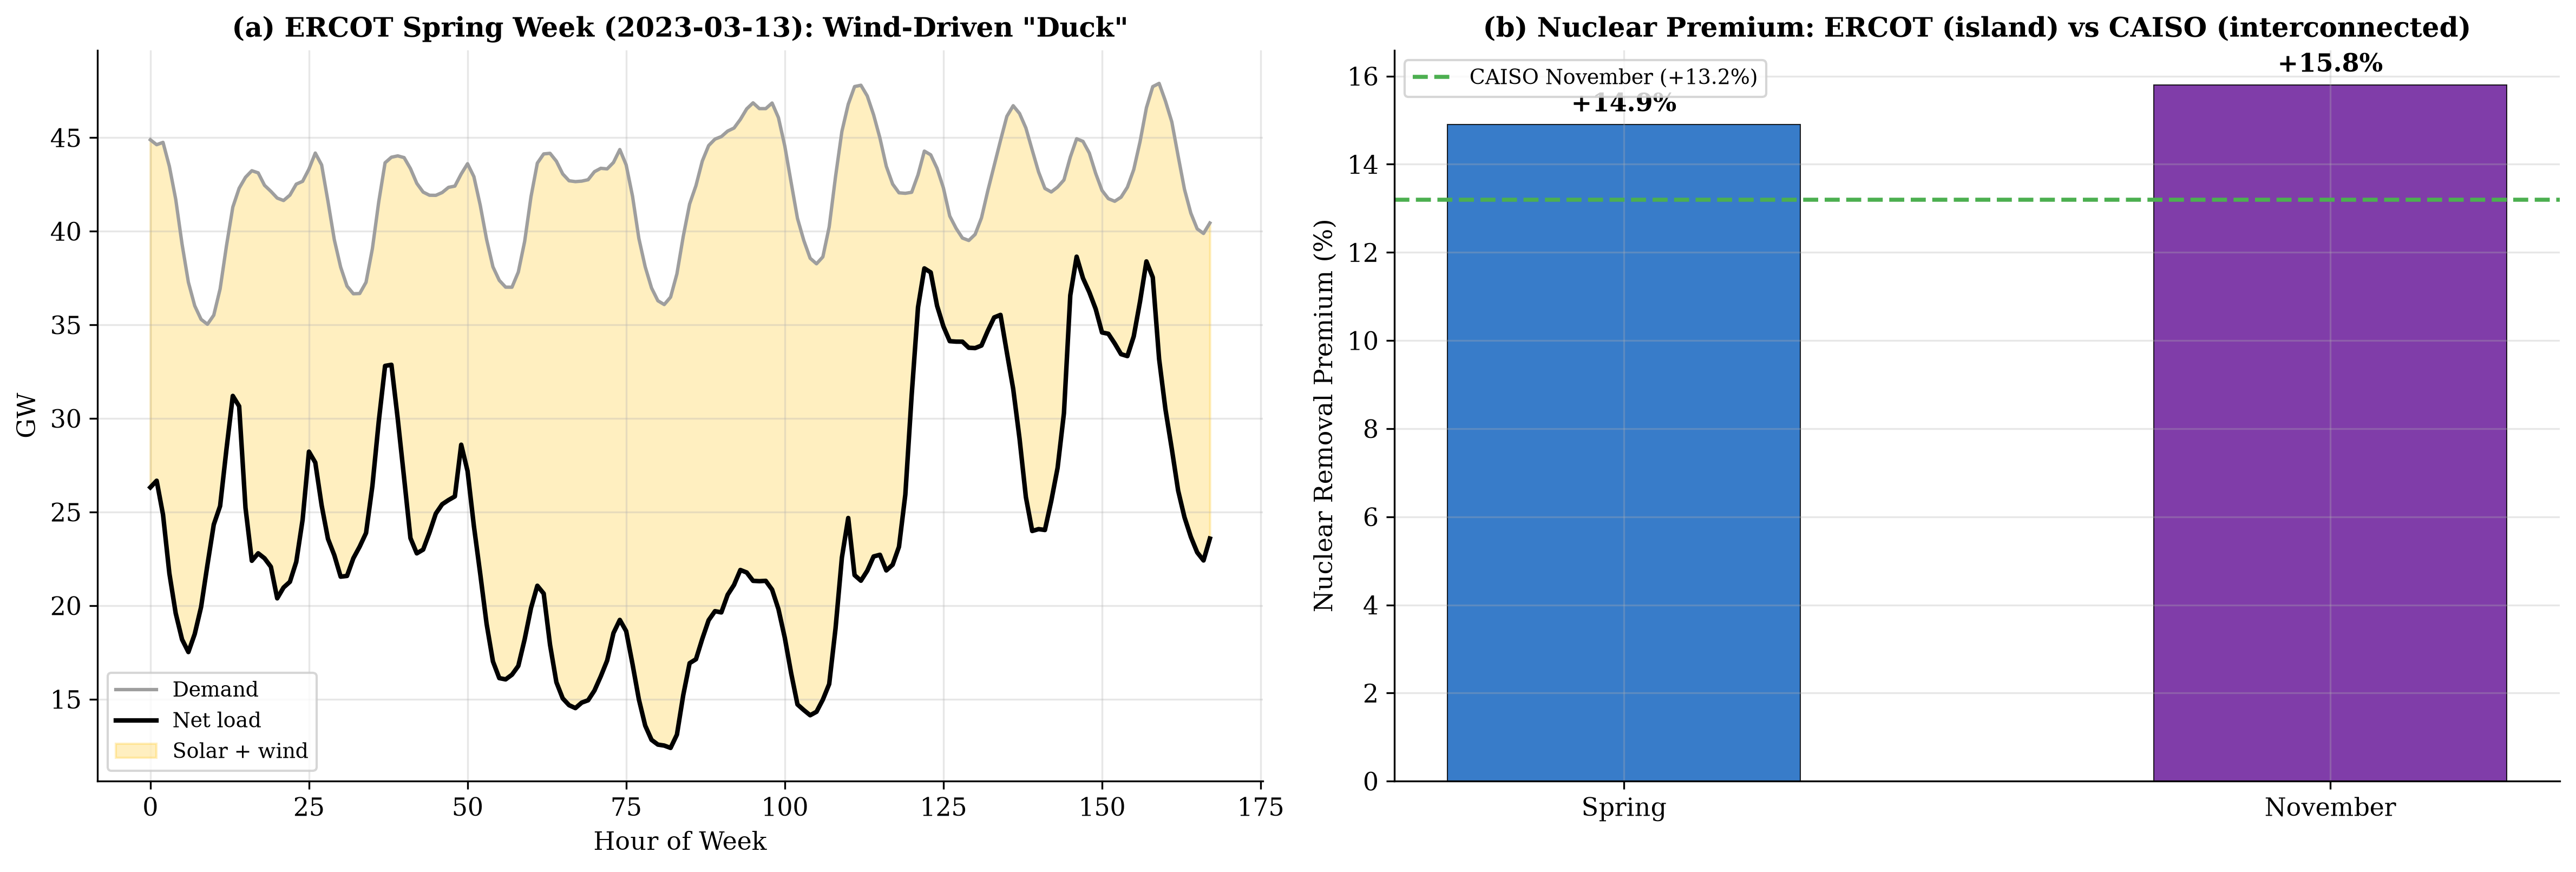
\includegraphics[width=\textwidth]{fig_ercot_case.png}
\caption{Supplementary ERCOT transferability check. (a) Wind-driven net load profile for the ERCOT spring week. (b) Nuclear removal premium in ERCOT (island topology, 1.22~GW ties) vs.\ the CAISO November baseline (10~GW imports), consistent with the hypothesis that scarce import capacity amplifies the nuclear premium.}
\label{fig:ercot}
\end{figure}


%% ====================================================================
%% REFERENCES
%% ====================================================================

\begin{thebibliography}{99}

\bibitem[Angelopoulos and Bates(2023)]{angelopoulos2023}
Angelopoulos, A.N., Bates, S., 2023. Conformal prediction: A gentle introduction. \textit{Foundations and Trends in Machine Learning} 16(4), 494--591.

\bibitem[Bergmeir and Ben\'itez(2012)]{bergmeir2012}
Bergmeir, C., Ben\'itez, J.M., 2012. On the use of cross-validation for time series predictor evaluation. \textit{Information Sciences} 191, 192--213.

\bibitem[Bertsimas and Sim(2004)]{bertsimas2004}
Bertsimas, D., Sim, M., 2004. The price of robustness. \textit{Operations Research} 52(1), 35--53.

\bibitem[Bertsimas et al.(2013)]{bertsimas2013}
Bertsimas, D., Litvinov, E., Sun, X.A., Zhao, J., Zheng, T., 2013. Adaptive robust optimization for the security constrained unit commitment problem. \textit{IEEE Transactions on Power Systems} 28(1), 52--63.

\bibitem[Bienstock et al.(2014)]{bienstock2014}
Bienstock, D., Chertkov, M., Harnett, S., 2014. Chance-constrained optimal power flow: Risk-aware network control under uncertainty. \textit{SIAM Review} 56(3), 461--495.

\bibitem[Birge and Louveaux(2011)]{birge2011}
Birge, J.R., Louveaux, F., 2011. \textit{Introduction to Stochastic Programming}, second ed. Springer, New York.

\bibitem[Bistline et al.(2023)]{bistline2023}
Bistline, J.E.T., Mehrotra, N.R., Wolfram, C., 2023. Economic implications of the climate provisions of the Inflation Reduction Act. \textit{Brookings Papers on Economic Activity} 2023(1), 77--157.

\bibitem[Breiman(2001)]{breiman2001}
Breiman, L., 2001. Random forests. \textit{Machine Learning} 45(1), 5--32.

\bibitem[CARB(2023)]{carb2023}
California Air Resources Board, 2023. Mandatory Greenhouse Gas Reporting Regulation: Default emission factor for unspecified imported electricity. Sacramento, CA.

\bibitem[CAISO(2016)]{caiso2016}
California Independent System Operator, 2016. What the duck curve tells us about managing a green grid. Technical report, Folsom, CA.

\bibitem[CAISO(2023)]{caiso2023}
California Independent System Operator, 2023. 2023 Annual Report on Market Issues and Performance. Department of Market Monitoring, Folsom, CA.

\bibitem[California State Legislature(2022)]{sb846}
California State Legislature, 2022. Senate Bill No.~846: Diablo Canyon powerplant --- extension of operations. Sacramento, CA.

\bibitem[Cany et al.(2018)]{cany2018}
Cany, C., Mansilla, C., Mathonni\`ere, G., da Costa, P., 2018. Nuclear power supply: Going against the misconceptions. Evidence of nuclear flexibility from the French experience. \textit{Energy} 151, 289--296.

\bibitem[Chen and Guestrin(2016)]{chen2016}
Chen, T., Guestrin, C., 2016. XGBoost: A scalable tree boosting system. In: \textit{Proceedings of the 22nd ACM SIGKDD International Conference on Knowledge Discovery and Data Mining}, pp.~785--794.

\bibitem[Conejo et al.(2010)]{conejo2010}
Conejo, A.J., Carri\'on, M., Morales, J.M., 2010. \textit{Decision Making Under Uncertainty in Electricity Markets}. Springer, New York.

\bibitem[Denholm et al.(2015)]{denholm2015}
Denholm, P., O'Connell, M., Brinkman, G., Jorgenson, J., 2015. Overgeneration from solar energy in California: A field guide to the duck chart. Technical Report NREL/TP-6A20-65023, National Renewable Energy Laboratory.

\bibitem[Denholm et al.(2022)]{denholm2022b}
Denholm, P., Brown, P., Cole, W., Mai, T., Sergi, B., et al., 2022. Examining supply-side options to achieve 100\% clean electricity by 2035. Technical Report NREL/TP-6A40-81644, National Renewable Energy Laboratory, Golden, CO.

\bibitem[Diebold and Mariano(1995)]{diebold1995}
Diebold, F.X., Mariano, R.S., 1995. Comparing predictive accuracy. \textit{Journal of Business \& Economic Statistics} 13(3), 253--263.

\bibitem[Dvorkin(2020)]{dvorkin2019}
Dvorkin, Y., 2020. A chance-constrained stochastic electricity market. \textit{IEEE Transactions on Power Systems} 35(4), 2993--3003.

\bibitem[ERCOT(2023)]{ercot2023}
Electric Reliability Council of Texas, 2023. 2023 Capacity, Demand and Reserves (CDR) Report. Austin, TX.

\bibitem[Gibbs and Cand\`es(2021)]{gibbs2021}
Gibbs, I., Cand\`es, E., 2021. Adaptive conformal inference under distribution shift. In: \textit{Advances in Neural Information Processing Systems} 34.

\bibitem[Gneiting and Raftery(2007)]{gneiting2007}
Gneiting, T., Raftery, A.E., 2007. Strictly proper scoring rules, prediction, and estimation. \textit{Journal of the American Statistical Association} 102(477), 359--378.

\bibitem[Grinsztajn et al.(2022)]{grinsztajn2022}
Grinsztajn, L., Oyallon, E., Varoquaux, G., 2022. Why do tree-based models still outperform deep learning on typical tabular data? In: \textit{Advances in Neural Information Processing Systems} 35.

\bibitem[Hart et al.(2017)]{hart2017}
Hart, W.E., Laird, C.D., Watson, J.-P., Woodruff, D.L., Hackebeil, G.A., Nicholson, B.L., Siirola, J.D., 2017. \textit{Pyomo---Optimization Modeling in Python}, second ed. Springer, New York.

\bibitem[Hertel et al.(2023)]{hertel2022}
Hertel, M., Beichter, M., Heidrich, B., Neumann, O., Sch\"afer, B., Mikut, R., Hagenmeyer, V., 2023. Transformer training strategies for forecasting multiple load time series. \textit{Energy Informatics} 6(Suppl 1), 20.

\bibitem[Hong and Fan(2016)]{hong2016}
Hong, T., Fan, S., 2016. Probabilistic electric load forecasting: A tutorial review. \textit{International Journal of Forecasting} 32(3), 914--938.

\bibitem[Hong et al.(2020)]{hong2020review}
Hong, T., Pinson, P., Wang, Y., Weron, R., Yang, D., Zareipour, H., 2020. Energy forecasting: A review and outlook. \textit{IEEE Open Access Journal of Power and Energy} 7, 376--388.

\bibitem[Huangfu and Hall(2018)]{huangfu2018}
Huangfu, Q., Hall, J.A.J., 2018. Parallelizing the dual revised simplex method. \textit{Mathematical Programming Computation} 10(1), 119--142.

\bibitem[Jenkins et al.(2018)]{jenkins2018}
Jenkins, J.D., Zhou, Z., Ponciroli, R., Vilim, R.B., Ganda, F., de Sisternes, F., Botterud, A., 2018. The benefits of nuclear flexibility in power system operations with renewable energy. \textit{Applied Energy} 222, 872--884.

\bibitem[Kath and Ziel(2021)]{kath2021}
Kath, C., Ziel, F., 2021. Conformal prediction interval estimation and applications to day-ahead and intraday power markets. \textit{International Journal of Forecasting} 37(2), 777--799.

\bibitem[Kaur et al.(2016)]{kaur2016}
Kaur, A., Nonnenmacher, L., Coimbra, C.F.M., 2016. Net load forecasting for high renewable energy penetration grids. \textit{Energy} 114, 1073--1084.

\bibitem[Ke et al.(2017)]{ke2017}
Ke, G., Meng, Q., Finley, T., Wang, T., Chen, W., Ma, W., Ye, Q., Liu, T.-Y., 2017. LightGBM: A highly efficient gradient boosting decision tree. In: \textit{Advances in Neural Information Processing Systems} 30.

\bibitem[Keefer and Bodily(1983)]{keefer1983}
Keefer, D.L., Bodily, S.E., 1983. Three-point approximations for continuous random variables. \textit{Management Science} 29(5), 595--609.

\bibitem[Koenker(2005)]{koenker2005}
Koenker, R., 2005. \textit{Quantile Regression}. Cambridge University Press, Cambridge.

\bibitem[Lago et al.(2021)]{lago2021}
Lago, J., Marcjasz, G., De Schutter, B., Weron, R., 2021. Forecasting day-ahead electricity prices: A review of state-of-the-art algorithms, best practices and an open-access benchmark. \textit{Applied Energy} 293, 116983.

\bibitem[Morales et al.(2014)]{morales2014}
Morales, J.M., Conejo, A.J., Madsen, H., Pinson, P., Zugno, M., 2014. \textit{Integrating Renewables in Electricity Markets: Operational Problems}. Springer, New York.

\bibitem[NREL(2023)]{nrelatb2023}
National Renewable Energy Laboratory, 2023. Annual Technology Baseline 2023. Golden, CO. \url{https://atb.nrel.gov}.

\bibitem[NEA(2011)]{nea2011}
Nuclear Energy Agency, 2011. Technical and Economic Aspects of Load Following with Nuclear Power Plants. OECD NEA No.~6786, Paris.

\bibitem[Papavasiliou and Oren(2013)]{papavasiliou2011}
Papavasiliou, A., Oren, S.S., 2013. Multiarea stochastic unit commitment for high wind penetration in a transmission constrained network. \textit{Operations Research} 61(3), 578--592.

\bibitem[Romano et al.(2019)]{romano2019}
Romano, Y., Patterson, E., Cand\`es, E., 2019. Conformalized quantile regression. In: \textit{Advances in Neural Information Processing Systems} 32.

\bibitem[Schmidt et al.(2019)]{schmidt2019}
Schmidt, O., Melchior, S., Hawkes, A., Staffell, I., 2019. Projecting the future levelized cost of electricity storage technologies. \textit{Joule} 3(1), 81--100.

\bibitem[Sepulveda et al.(2018)]{sepulveda2018}
Sepulveda, N.A., Jenkins, J.D., de Sisternes, F.J., Lester, R.K., 2018. The role of firm low-carbon electricity resources in deep decarbonization of power generation. \textit{Joule} 2(11), 2403--2420.

\bibitem[Sioshansi et al.(2009)]{sioshansi2009}
Sioshansi, R., Denholm, P., Jenkin, T., Weiss, J., 2009. Estimating the value of electricity storage in PJM: Arbitrage and some welfare effects. \textit{Energy Economics} 31(2), 269--277.

\bibitem[EPA(2024)]{epa2023}
U.S.\ Environmental Protection Agency, 2024. Emissions \& Generation Resource Integrated Database (eGRID) 2022. Washington, DC.

\bibitem[Vovk et al.(2005)]{vovk2005}
Vovk, V., Gammerman, A., Shafer, G., 2005. \textit{Algorithmic Learning in a Random World}. Springer, New York.

\bibitem[Weron(2014)]{weron2014}
Weron, R., 2014. Electricity price forecasting: A review of the state-of-the-art with a look into the future. \textit{International Journal of Forecasting} 30(4), 1030--1081.

\bibitem[Zaffran et al.(2022)]{zaffran2022}
Zaffran, M., F\'eron, O., Goude, Y., Josse, J., Dieuleveut, A., 2022. Adaptive conformal predictions for time series. In: \textit{Proceedings of the 39th International Conference on Machine Learning}, PMLR 162, pp.~25834--25866.

\end{thebibliography}

\end{document}
